%%
% The BIThesis Template for Bachelor Graduation Thesis
%
% 北京理工大学毕业设计(论文) —— 使用 XeLaTeX 编译
%
% Copyright 2021-2023 BITNP
%
% This work may be distributed and/or modified under the
% conditions of the LaTeX Project Public License, either version 1.3
% of this license or (at your option) any later version.
% The latest version of this license is in
%   http://www.latex-project.org/lppl.txt
% and version 1.3 or later is part of all distributions of LaTeX
% version 2005/12/01 or later.
%
% This work has the LPPL maintenance status `maintained'.
%
% The Current Maintainer of this work is Feng Kaiyu.
%
% Compile with: xelatex -> biber -> xelatex -> xelatex

% !TeX program = xelatex
% !BIB program = biber


% 开启盲审格式 blindPeerReview=true (如:[type=bachelor,blindPeerReview=true])

% 正常格式
\documentclass[type=bachelor]{bithesis}
% 盲审格式
% \documentclass[type=bachelor,blindPeerReview=true]{bithesis}

\BITSetup{
  cover = {
    % 在封面中载入有「北京理工大学」字样的图片,如无必要请勿改动。
    headerImage = images/header.png,
    % 在封面标题中使用思源黑体,使用此选项可以保证与 Word 封面标题的字体一致。
    xiheiFont = STXIHEI.TTF,
    %% 使用以下参数来自定义封面日期
    % date = 2022年6月,
  },
  info = {
    % 想要删除某项封面信息,直接删除该项即可。
    % 想要让某项封面信息留空(但是保留下划线),请设置为空字符串。
    % 如需要换行,则用 “\\” 符号分割。
    title = 基于区块链的出租车调度系统的完善,
    titleEn = {The perfection of the taxi dispatching system based on blockchain},
    school = 计算机学院,
    major = 计算机科学与技术,
    class = 07111908,
    author = 蒙思洁,
    studentId = 1120193602,
    supervisor = 陆慧梅,
    keywords = {区块链;出租车调度系统;A*算法;实时路况计算},
    keywordsEn = {Blockchain;The Taxi dispatching system; Astar algorithm;Real-time traffic situation estimation},
    % 如果你的毕设为校外毕设,请将下面这一行语句解除注释(删除第一个百分号字符)并填写你的校外毕设导师名字
    % externalSupervisor = 左偏树,
  },
  style = {
    % 保持参考文献的缩进样式与 Word 模板一致。
    % 如果你不需要此样式,请将此行注释掉。
    bibliographyIndent = false,
  }
}

% 使用 listings 宏包进行代码块使用,并使用了预定义的样式,
% 你也可以选用自己的喜欢的其他宏包,如 minted;
% 然而由于 minted 依赖 Python 的 Pygments 库作为外部依赖,因此出于模板的简洁程度考虑,我们没有提供 minted 进行代码块书写的示例。
\usepackage{listings}
\usepackage{minted}
% ---插入多行注释的包---
\usepackage{verbatim}
% ---插入三线表的包---
\usepackage{makecell}
\usepackage{geometry}
\usepackage{tabularx}
\usepackage{array}

% ---插入代码块的包---
\usepackage{listings}
\usepackage{xcolor}

% ---插入超链接的包---
% \usepackage[colorlinks,linkcolor=blue]{hyperref}


\usepackage[
  backend=biber,
  style=gb7714-2015,
  gbalign=gb7714-2015,
  gbnamefmt=lowercase,
  gbpub=false,
  doi=false,
  url=false,
  eprint=false,
  isbn=false,
]{biblatex}

% 参考文献引用文件位于 misc/ref.bib
\addbibresource{misc/ref.bib}


% 文档开始
\begin{document}

% 标题页面:如无特殊需要,本部分无需改动
% \input{misc/0_cover.tex}
\MakeCover

% 原创性声明:如无特殊需要,本部分无需改动
% 更改为 PDF 页面插入,如需要添加内容,可考虑先用 Word 制作再覆盖 misc/1_originality.pdf
% ====== 原创性声明(PDF 格式)======
\begin{blindPeerReview}
  
\includepdf{misc/1_originality.pdf}\newpage
\end{blindPeerReview}
% ====== 原创性声明(PDF 格式)======
% ====== 原创性声明(LaTeX 格式)======
% %%
% The BIThesis Template for Bachelor Graduation Thesis
%
% 北京理工大学毕业设计(论文)原创性声明模板 —— 使用 XeLaTeX 编译
%
% Copyright 2020-2023 BITNP
%
% This work may be distributed and/or modified under the
% conditions of the LaTeX Project Public License, either version 1.3
% of this license or (at your option) any later version.
% The latest version of this license is in
%   http://www.latex-project.org/lppl.txt
% and version 1.3 or later is part of all distributions of LaTeX
% version 2005/12/01 or later.
%
% This work has the LPPL maintenance status `maintained'.
%
% The Current Maintainer of this work is Feng Kaiyu.
%
% Compile with: xelatex -> biber -> xelatex -> xelatex
%
% 如无特殊需要,本页面无需更改

\MakeOriginality

% ====== 原创性声明(LaTeX 格式)======

% 前置页面定义
\frontmatter
% 摘要:在摘要相应的 TeX 文件处进行摘要部分的撰写
% %%
% The BIThesis Template for Bachelor Graduation Thesis
%
% 北京理工大学毕业设计(论文)中英文摘要 —— 使用 XeLaTeX 编译
%
% Copyright 2020-2023 BITNP
%
% This work may be distributed and/or modified under the
% conditions of the LaTeX Project Public License, either version 1.3
% of this license or (at your option) any later version.
% The latest version of this license is in
%   http://www.latex-project.org/lppl.txt
% and version 1.3 or later is part of all distributions of LaTeX
% version 2005/12/01 or later.
%
% This work has the LPPL maintenance status `maintained'.
%
% The Current Maintainer of this work is Feng Kaiyu.

% 中英文摘要章节
\begin{abstract}
% 中文摘要正文从这里开始
本文……。

\textcolor{blue}{摘要正文选用模板中的样式所定义的“正文”,每段落首行缩进 2 个字符;或者手动设置成每段落首行缩进 2 个汉字,字体:宋体,字号:小四,行距:固定值 22 磅,间距:段前、段后均为 0 行。阅后删除此段。}

\textcolor{blue}{摘要是一篇具有独立性和完整性的短文,应概括而扼要地反映出本论文的主要内容。包括研究目的、研究方法、研究结果和结论等,特别要突出研究结果和结论。中文摘要力求语言精炼准确,本科生毕业设计(论文)摘要建议 300-500 字。摘要中不可出现参考文献、图、表、化学结构式、非公知公用的符号和术语。英文摘要与中文摘要的内容应一致。阅后删除此段。}

\end{abstract}

% 英文摘要章节
\begin{abstractEn}
% 英文摘要正文从这里开始
In order to study……

\textcolor{blue}{Abstract 正文设置成每段落首行缩进 2 字符,字体:Times New Roman,字号:小四,行距:固定值 22 磅,间距:段前、段后均为 0 行。阅后删除此段。}
\end{abstractEn}

%%
% The BIThesis Template for Bachelor Graduation Thesis
%
% 北京理工大学毕业设计(论文)中英文摘要 —— 使用 XeLaTeX 编译
%
% Copyright 2020-2023 BITNP
%
% This work may be distributed and/or modified under the
% conditions of the LaTeX Project Public License, either version 1.3
% of this license or (at your option) any later version.
% The latest version of this license is in
%   http://www.latex-project.org/lppl.txt
% and version 1.3 or later is part of all distributions of LaTeX
% version 2005/12/01 or later.
%
% This work has the LPPL maintenance status `maintained'.
%
% The Current Maintainer of this work is Feng Kaiyu.

% 中英文摘要章节
\begin{abstract}
% 中文摘要正文从这里开始
汽车出行目前已成为我国社会的交通常态。当下,网约车便于用户预约车辆、实现点对点运输,能满足乘客个性化需求,成为许多人首要的出行方式。但其数据处理、存储均通过第三方平台完成,依赖中心服务器,使数据安全无法得到保证。将区块链与车联网工作结合,保证了司乘间可信交流,提升了打车平台的数据安全性。

本文在实验室前期工作的基础上,调研了树状区块链、Geohash编码、A*算法原理、实时路况计算等技术。本文还复现了实验室前期设计的支持区域划分的树状区块链和出租车调度系统,处理了向区块链上传的北京真实地图数据,从而更新了出租车调度系统中的地图数据。针对实验室已实现的静态路径规划算法,本文提出了基于实时路况的改进A*算法,并将其应用于出租车调度系统。此外,本文对该完善后的出租车调度系统进行了运行测试和性能测试。测试表明,完善后的系统实现了合理的动态路径规划功能,其中改进的A*算法复杂度良好,这证明了本文把基于实时路况的改进A*算法引入出租车调度系统的工作具有可行性。本文工作完善了出租车调度系统的路径规划机制,对真实的出租车调度过程进行了一定程度上的模拟,具有较高实用价值。

\end{abstract}

% 英文摘要章节
\begin{abstractEn}
% 英文摘要正文从这里开始
Car travel has become a normal traffic in our society. At present, online car booking is convenient for users to book a car and realize point-to-point transportation. It can meet the personalized needs of passengers, and has become the primary mode of travel for many people. However, its data processing and storage are completed through the third party platform, relying on the central server, so that the data security can not be guaranteed. The combination of blockchain and Internet of vehicles ensures reliable communication between drivers and passengers, and improves the data security of the ride-hailing platform. 

Based on the previous work in the laboratory, this thesis investigated tree blockchain, Geohash coding technology, A* algorithm principle, real-time traffic situation estimation and other technologies. This thesis reproduces the tree-based blockchain supporting regional division designed by the laboratory earlier, and reproduces the taxi dispatching system based on it. This thesis also processed the real map data of Beijing uploaded to the blockchain, thus updating the map data in the taxi dispatching system. Aiming at the static path planning algorithm realized in the laboratory, this thesis proposes an improved A* algorithm based on real-time traffic situation and applies it to the taxi dispatching system. In addition, this thesis carries on the running test and the performance test of the improved taxi dispatching system. The test results show that the perfected system can realize reasonable dynamic path planning function, and the improved A* algorithm is of good complexity, which proves that it is feasible to introduce the improved A* algorithm based on real-time traffic situation into the taxi dispatching system in this thesis. This thesis improves the route planning mechanism of taxi dispatching system and simulates the real taxi dispatching process to a certain extent, which has high practical value.

\end{abstractEn}


\MakeTOC

% 正文开始
\mainmatter

% 第一章
\chapter{绪论}

\section{研究背景}

\space 近年来,随着经济社会的飞速发展,我国全面跨入汽车社会,汽车出行成为交通常态。据公安部统计,目前,我国驾驶人数量占成年人数量近 50%,平均每 2 个成年人中即有 1 人持有驾驶证。与此同时,汽车保有量同步迅猛增长,全国汽车保有量超过 3 亿辆,平均每百户家庭拥有汽车达到 60 辆\cite{驾驶人数据}。汽车走进千家万户,成为了普通家庭出行的常用选择之一。驾驶技能已经变成了家家户户的基本生活技能,带给交通道路的车流压力也与日俱增。

\space 在``出行难”问题横亘的当下,面对出行限号、停车位少等现实问题,共享单车、公交地铁、出租车等成为人们出行的首要选择。较共享单车来说,出租车不受车辆本身实物的限制;较公交地铁来说,出租车更加灵活便捷,能更快速地完成人们出行的需求。

\space 在传统的出租车出行领域中,存在着乘客等候时间长、司机挑客绕路、乘车环境差等问题\cite{赵杨2022网约车冲击下出租车行业转型对策研究}。随着互联网的不断发展,网络平台公司将车辆接入互联网平台,用户通过使用网络平台公司提供的手机软件,预约车辆,实现点对点运输,并对车辆进行评价反馈。网约车的兴起,极大满足了乘客个性化、便捷化的出行需求。

\space 车载网是一种特殊的移动自组织网络,它通过汽车收集、共享信息,实现更加智能、安全的驾驶\cite{程刚2011车联网现状与发展研究}。安全性和可靠性是车载网关注的主要问题\cite{Zhaojun2018A}。区块链技术具有去中心化、时序数据、集体维护、可编程和安全可信等特点\cite{袁勇2016区块链技术发展现状与展望}。因此,区块链满足分布式数据存储的需求,能为车载网数据传输的安全性、可追溯性提供技术保障、隐私保护。将区块链技术和车载网工作融合,形成一个基于区块链的出租车调度系统。区块链技术中数据信息不可篡改,因此应用进网约车系统中可以提升通讯的安全性,保证平台无法垄断打车数据,保证信息公开透明。司机与乘客之间进行直接交流与贸易,保证了司乘双方的可信交流。车与车之间进行位置通讯,也能提高通讯传输效率,营造安全高效的打车服务。

\section{相关工作}

\subsection{区块链和智能合约}

\space 在互联网上进行的电子支付活动大多数都依赖于可信第三方,但这种方式仍存在一定的风险。完全不可逆的交易不现实,调解纠纷导致的调解成本也会增加交易成本,从而使小额随机交易无法进行。因此,需要一种能允许任意两方直接交易的基于加密证明的机制,来更新现有的依赖可信第三方的电子支付方式。

\space 中本聪在2008年提出区块链技术,其在文献中描述区块链为按照时间顺序将数据区块以链条的方式组合成特定数据结构,并以密码学方式保证的不篡改和不可伪造的去中心化共享总账\cite{2008Bitcoin}。区块链采用纯数学的方法,无需可信第三方,也不牺牲隐私性,对过去、当前的数字事件建立分布式的一致性表达\cite{袁勇2016区块链技术发展现状与展望}。区块链也提供了可编程的脚本系统,增强了区块链应用的灵活性\cite{贺海武2018基于区块链的智能合约技术与应用综述}。

区块链技术目前已应用发展了三个阶段\cite{swan2015blockchain}:

\begin{enumerate}
    \item 区块链1.0:可编程货币,以比特币为代表,是数字货币应用。
    \item 区块链2.0:可编程金融,以智能合约为代表,将数字货币与智能合约结合,主要在金融领域中应用。
    \item 区块链3.0:可编程社会,为各行各业提供去中心化应用、去中心化自组织等解决方案。
\end{enumerate}

智能合约在1994年首次被Nick Szabo提出\cite{1997Formalizing}。它被定义为``一套以数字形式指定的承诺,包括合约参与方可以在其上执行这些承诺的协议”。2013年12月,Vitalik Buterin提出了以太坊区块链平台,提供了可编写智能合约的图灵完备的编程语言,才首次将智能合约与区块链技术相结合,并投入应用\cite{2014ASmartContract}。

智能合约是部署在区块链上的程序。它是可自动执行的脚本,一旦满足预先设定的条件,就可以立刻自动运行,从而使参与者不需要任何机构介入,就能获取合约运行结果。以太坊通过配备的智能合约实现任何人都可以创建的去中心化应用程序,吸引了大量开发者投入此平台,促进了一系列新型产业发展。以太坊的出现促使区块链与智能合约不再局限于数字货币,从而将区块链与智能合约的应用推广到金融领域和其他社会领域\cite{欧阳丽炜2019智能合约}。智能合约的代码语句易懂,当预定条件满足且完成验证后,区块链将执行相应行为,如释放资金、发出凭证,并在交易完成时,更新区块链。本文课题基于以太坊部署智能合约,并在此基础上,进行出租车调度系统的深入研究。

\subsection{Geohash编码技术}

移动用户的增加,提升了交互式信息地图的服务需求,促进了矢量数据地图的兴起。传统的矢量地图有Google Maps\cite{2015ggmap},它采用二维的经纬度数据表示一个唯一的地理位置。Geohash是一类新型的地址编码方式,它的编码过程如下:将经纬度分别转换成二进制字符串,将这一对二进制字符串按位交叉,奇数位为纬度序列,偶数位为经度序列,从而得到一组新字符串,将新字符串转换为十进制,并使用Base32编码方式处理该十进制字符串,从而获得该地理位置对应的Geohash编码字符串\cite{2018HGeoHashBase}。

将道路``北蜂窝路”中的经纬度(116.3227718,39.9037387)使用Geohash编码技术编码为wx4enbr8jh1的一部分过程如附录中的表\ref{geohash-weidu}和表\ref{geohash-jingdu}。

\iffalse
% 设置三线表
\begin{table}[ht]
    \linespread{1.5}
    \zihao{5}
    \centering
    \caption{纬度的二进制表示过程}
    \label{geohash-weidu}
    \begin{tabularx}{\textwidth}{XXXc}
    \toprule
    纬度 & 划分区间0 & 划分区间1 & 39.9037387 \\
    \hline
    (-90,90) & (-90,0) & (0,90) & 1 \\
    (0,90) & (0,45) & (45,90) & 0 \\
    (0,45) & (0,22.5) & (22.5,45) & 1 \\
    (22.5,45) & (22.5,33.75) & (33.75,45) & 1 \\
    (33.75,45) & (33.75,39.375) & (39.375,45) & 1 \\
    (39.375,45) & (39.375,42.1875) & (42.1875,45) & 0 \\
    (39.375,\newline 42.1875) & (39.375,\newline 40.78125) & (40.78125,\newline 42.1875) & 0 \\
    (39.375,\newline 40.78125) & (39.375,\newline 40.078125) & (40.078125,\newline 40.78125) & 0 \\
    (39.375,\newline 40.078125) & (39.375,\newline 39.7265625) & (39.7265625,\newline 40.078125) & 1 \\
    (39.7265625,\newline 40.078125) & (39.7265625,\newline 39.90234375) & (39.90234375,\newline 40.078125) & 1 \\
    (39.90234375,\newline 40.078125) & (39.90234375,\newline 39.990234375) & (39.990234375,\newline 40.078125) & 0 \\
    (39.90234375,\newline 39.990234375) & (39.90234375,\newline 39.9462890625) & (39.9462890625,\newline 39.990234375) & 0 \\
    (39.90234375,\newline 39.9462890625) & (39.90234375,\newline 39.92431640625) & (39.92431640625,\newline 39.9462890625) & 0 \\
    (39.90234375,\newline 39.92431640625) & (39.90234375,\newline 39.913330078125) & (39.913330078125,\newline 39.92431640625) & 0 \\
    (39.90234375,\newline 39.913330078125) & (39.90234375,\newline 39.9078369140625) & (39.9078369140625,\newline 39.913330078125) & 0 \\
    \bottomrule
    \end{tabularx}
\end{table}
% 结束设置三线表

% 设置三线表
\begin{table}[ht]
    \linespread{1.5}
    \zihao{5}
    \centering
    \caption{经度的二进制表示过程}
    \label{geohash-jingdu}
    \begin{tabularx}{\textwidth}{XXXc}
    \toprule
    纬度 & 划分区间0 & 划分区间1 & 116.3227718 \\
    \hline
    (-180,180) & (-180,0) & (0,180) & 1\\
    (0,180) & (0,90) & (90,180) & 1\\
    (90,180) & (90,135) & (135,180) & 0\\
    (90,135) & (90,112.5) & (112.5,135) & 1\\
    (112.5,135) & (112.5,123.75) & (123.75,135) & 0\\
    (112.5,123.75) & (112.5,118.125) & (118.125,123.75) & 0\\
    (112.5,118.125) & (112.5,115.3125) & (115.3125,118.125) & 1\\
    (115.3125,\newline 118.125) & (115.3125,\newline 116.71875) & (116.71875,\newline 118.125) & 0\\
    (115.3125,\newline 116.71875) & (115.3125,\newline 116.015625) & (116.015625,\newline 116.71875) & 1\\
    (116.015625,\newline 116.71875) & (116.015625,\newline 116.3671875) & (116.3671875,\newline 116.71875) & 0\\
    (116.015625,\newline 116.3671875) & (116.015625,\newline 116.19140625) & (116.19140625,\newline 116.3671875) & 1\\
    (116.19140625,\newline 116.3671875) & (116.19140625,\newline 116.279296875) & (116.279296875,\newline 116.3671875) & 1\\
    (116.279296875,\newline 116.3671875) & (116.279296875,\newline 116.3232421875) & (116.3232421875,\newline 116.3671875) & 0\\
    (116.279296875,\newline 116.3232421875) & (116.279296875,\newline 116.30126953125) & (116.30126953125,\newline 116.3232421875) & 1\\
    (116.30126953125,\newline 116.3232421875) & (116.30126953125,\newline 116.312255859375) & (116.312255859375,\newline 116.3232421875) & 1\\
    \bottomrule
    \end{tabularx}
\end{table}
% 结束设置三线表
\fi

通过对经纬度不断进行二分比对操作,得到``北蜂窝路”的纬度二进制序列为101110001100000,经度二进制序列为110100101011011,按照纬度为奇数位,经度为偶数位的方式,将经纬度序列排列成一个二进制序列为111001110100100011011010001010,每五位转为十进制,得到数字28,29,4,13,20,10,用表\ref{base32}中的Base32编码进行转换后得到wx4enb。
% 设置三线表
\begin{table}[ht]
    \linespread{1.5}
    \zihao{5}
    \centering
    \caption{Base32编码转换}
    \label{base32}
    \begin{tabular}{ccccccccccccccccc}
    \toprule
    Demical & 0 & 1 & 2 & 3 & 4 & 5 & 6 & 7 & 8 & 9 & 10 & 11 & 12 & 13 & 14 & 15 \\
    Base32 & 0 & 1 & 2 & 3 & 4 & 5 & 6 & 7 & 8 & 9 & b & c & d & e & f & g \\
    Demical & 16 & 17 & 18 & 19 & 20 & 21 & 22 & 23 & 24 & 25 & 26 & 27 & 28 & 29 & 30 & 31 \\
    Base32 & h & j & k & m & n & p & q & r & s & t & u & v & w & x & y & z \\
    \bottomrule
    \end{tabular}
\end{table}
% 结束设置三线表

相比于传统的经纬度数据来说,Geohash编码方式将二维查询过程转换为一维字符串匹配,从而在查询性能的提升角度展现出了巨大的优势。Geohash可以实现时间复杂度为O(1)的快速查询,以Geohash编码为基础的空间索引算法针对海量地理数据也同样具有高性能查询能力\cite{2014AGeohash}。

从``北蜂窝路”的示例中可以得出结论,Geohash编码的精度与Geohash编码的位数有关,在本示例中,由于对经纬度各进行15次二分,因此得到的待使用Base32转换的二进制序列一共有30位数据,即对应6位Geohash编码。如果对经纬度各进行20次二分,则得到的待使用Base32转换的二进制序列将一共有40位数据,就会对应8位Geohash编码。该8位Geohash编码相较该6位Geohash的精度更高,且此6位编码与该8位编码的前6位编码数据完全相同,这也意味着一个GeoHash值所代表的区域,一定包含以该GeoHash值为前缀的所有元素。这是Geohash编码最重要的特征。

Geohash编码转换方式在编码长度恰当的情况下,误差是可接受的,如表1-1所示。
% 设置三线表
\begin{table}[ht]
    \linespread{1.5}
    \zihao{5}
    \centering
    \caption{不同长度Geohash编码的误差}
    \label{geo1}
    \begin{tabular}{cccc}
    \toprule
    Geohash length & Lat.err & Lon.err & Km.err \\
    \hline
    1 & ±3 & ±23 & ±2500 \\
    2 & ±2.8 & ±5.6 & ±630 \\
    3 & ±0.7 & ±0.70 & ±78 \\
    4 & ±0.087 & ±0.18 & ±20 \\
    5 & ±0.022 & ±0.022 & ±2.4 \\
    6 & ±0.0027 & ±0.0055 & ±0.61 \\
    7 & ±0.00068 & ±0.00068 & ±0.076 \\
    8 & ±0.000085 & ±0.00017 & ±0.019 \\
    \bottomrule
    \end{tabular}
\end{table}
% 结束设置三线表

Geohash将地理位置根据方格进行划分,适用于车辆调度的相关应用场景。栾方军、张鹏旭、曹科研提出了一种空载出租车巡游路线推荐模型,该模型利用8位长度的Geohash编码,结合地图路网数据,实时预测空载的出租车司机在行驶过程中周边发出打车订单的乘客数量,大幅提高出租车的载客率\cite{栾方军2020Geohash}。

本文课题所依赖的出租车调度系统基于Geohash编码。该系统将Geohash编码方式应用于地图存储与可视化上,并将用Geohash编码方式转换过的车辆与乘客地理位置信息作为区块属性存储,根据地理信息的层次性结构,形成树状区块结构,从而提升在传统区块链中匹配检索地理信息的效率。

\subsection{A*算法}

\space 交互式信息地图的出现,使用户能够即时在线判断自己周围的地理方位,更极大地便利了用户的出行体验。用户在出行时,可以根据交互式信息地图选取最合适自己的出行路径。路径规划方法也应需而生。最广泛的研究领域是最短路径规划,其又分为静态路径规划和动态路径规划。

\space 静态路径规划是在已存在的地理信息、交通规则等约束条件的作用下,寻找最短路径的一类算法。经典的静态路径规划算法有以下几类:

\begin{enumerate}
    \item Dijkstra算法:由Edsger Wybe Dijkstra在1956年提出,用来寻找图形中起点和重点间最短的路径\cite{1959A},即处理单源最短路径。Dijkstra算法以贪心思想为核心,从起点向外层层扩展,直至找到终点,时间复杂度为O(n²)。洪安定将Dijkstra算法与打车平台结合,并投入社会使用,产生了较好的效益\cite{洪安定基于优化司乘匹配的区域网约车平台设计与实现}。
    \item Floyd算法:由Floyd在1962年提出\cite{1962Algorithm},能正确处理有向图、负权的最短路径规划问题,也可以用于计算有向图的传递闭包,即可以处理多源最短路径和负权图,时间复杂度为O(n)。黄文团等基于Floyd算法实现了一个拼车信息服务系统,致力于缓解交通压力,满足城市居民的拼车需求\cite{黄文团2011}。
    \item A*算法:由PE Hart,NJ Nilsson,B Raphael在1968年提出\cite{1972A},它将Dijkstra算法与广度优先算法融合,借助启发式函数,更快找到最优路径,时间复杂度为O(n)。此算法精确稳定,常被使用在各种智能车路径规划场景中。
\end{enumerate}

\space 动态路径规划由Cooke和Halsey于1966年提出\cite{1966The},它根据特定类型的道路权值求解起终点间最短路径,并实时维护道路信息,即时调整预先规划好的最短路径。经典的动态路径规划算法有以下几类:

\begin{enumerate}
    \item DWA算法:由Fox D.和Burgard W.于1997年提出\cite{1997The},它将采样速度设计成一个动态窗口,在该窗口中有很多条可行轨迹,通过自行设计的评价函数评价这些轨迹,挑选出一条最优轨迹,重复迭代搜索当前最优轨迹,从而到达目的地。杨中华等\cite{杨中华0基于改进方向评价函数}对DWA算法的方向评价函数进行改进,为无人车的局部路径规划提供了一条解决方案。
    \item APF算法:由Oussama Khatib在1985年提出\cite{1986Real},它是一种反馈控制策略,通过目标的引理与障碍物的斥力共同引导机器人的移动。杜婉茹\cite{杜婉茹2021面向未知环境及动态障碍的人工势场路径规划算法}等将面向未知复杂环境的动态APF路径规划算法引入进模拟场景中进行仿真,获得了较好的寻路效果。
\end{enumerate}

\space 静态路径规划聚焦于全局规划,动态路径规划聚焦于局部规划,因此二者可以进行结合,协同工作,从而规划出局部最优、全局亦最优的路径。本文所基于的出租车调度系统,采用A*算法进行静态全局寻路,本文将实时路况引入调度系统,使其支持动态路径规划,并获得了较好效果。

\subsection{实时路况}

实时路况是描述一个城市交通道路的拥堵通畅状况的概念,实时路况对交通拥堵的预测具有重大意义\cite{何小波2021基于互联网地图的矢量路况数据生成与应用方法研究}。将实时路况引入出租车调度系统中,能更真实地模拟实际生活中的出租车调度场景,是非常有必要的。

实时路况的采集有以下四类方法\cite{何小波2021基于互联网地图的矢量路况数据生成与应用方法研究}:

\begin{enumerate}
    \item 人工采集:通过人工主动汇报其所在地路况,这种方法时效性低、有效覆盖范围小,费时费力,适合特定路段、特定时间段的路况采集。
    \item 传感器监测:通过道路上安装的摄像头、地感线圈、微波检测器等设备实时监测道路车流量,该方法监测的数据时效性和准确性高,但多由政府、机构掌握,难以共享。
    \item 浮动车法:通过浮动车上安装的GPS设备,实时记录浮动车的位置和速度,该方法监测的数据时效性和准确性高,但数据私有,共享难度大。
    \item 数据众包:通过众包模式获取数据,调用分散的用户各自提交数据,最终获得海量的数据。
\end{enumerate}

浮动车法相比其他几种方式,造价更低、覆盖范围更广,可以提供准确性高的车辆位置和速度信息,因此成为探测城市路况的一种重要数据来源\cite{孙卫真2019低采样率浮动车的路况计算精度优化}。

张禹\cite{张禹基于车辆轨迹的动态路况挖掘}使用基于OHMM的地图匹配算法,将浮动车轨迹与道路相匹配,从而便利路况计算。邱皓月\cite{孙卫真2019低采样率浮动车的路况计算精度优化}采用张禹的道路匹配算法,给出了一种精度更高的低采样率下浮动车的路况计算方法,有效地将实时路况与矢量地图数据进行结合,在考虑历史路况的影响下,使用历史路况对道路的实时路况进行加权平滑,精确推导实时路况。

本文将沿用邱皓月的实时路况计算思路,在本文课题所依赖的出租车调度系统中加入实时路况的影响因素,对属于静态路径规划范畴的A*算法进行优化,实现一个基于实时路况规划路径的出租车调度系统。

\section{本文研究内容、贡献和组织架构}

\subsection{本文研究内容及贡献}

首先,本文研究了传统区块链技术、周畅\cite{s22228885}实现的支持区域划分的树状区块链、智能合约;然后研究了Geohash编码技术的编码方式与特征;接下来研究了静态最短路径规划与动态最短路径规划这两种不同路径规划算法的优缺点与适用场景;最后研究了邱皓月\cite{孙卫真2019低采样率浮动车的路况计算精度优化}实现的实时路况推导过程。

接下来,本文进入数据准备阶段。本文完善了实验室的复现工作,实现了基于树状区块链的出租车调度系统的复现;本文还使用ArcGIS、PostgreSQL软件,结合2023年4月的北京地图数据,按不同Geohash编码划分地图区域,完成了wx4en、wx4er、wx4ep、wx4eq区域里北京真实地图数据的获取,并将地图数据中的经纬度编码为Geohash格式,成功上传到区块链中,更新了出租车调度系统中使用的地图。

紧接着,本文介绍了基于区块链的出租车调度系统的结构。然后本文选取了曼哈顿距离作为A*算法的启发函数,结合公式及场景示例,阐述了A*算法的工作原理及运行流程。在传统A*算法的基础上,本文还基于实时路况提出了结合实时路况的改进A*算法,结合公式及场景实例,阐明了改进A*算法的工作原理与运行流程,并指出了其在出租车调度系统中的实现方法,表明了这种改进A*算法投入应用的可行性。

本文完善的出租车调度系统相比于实验室过往工作中设计的出租车调度系统而言,最大的优势是引入了实时路况的影响因素,从而使该系统能够根据路况动态地规划路径,更接近于真实生活场景。

最后,本文先对地图数据进行了测试,保证上传给区块链的地图数据真实可信,具有可用性;接着,本文把基于实时路况的改进A*算法整合进出租车调度系统中,进行了运行测试与性能测试,证明了将本文所提出的改进A*算法应用在出租车调度系统中这一行为具有可行性。

\subsection{本文组织架构}

本文一共分为五部分,各部分主要内容如下:

第一章介绍了基于区块链的出租车调度系统的背景与意义,并对本文涉及的相关工作、国内外研究现状进行了综述,包括区块链技术和智能合约、Geohash编码、A*算法、实时路况计算,最后介绍了本文的研究内容与贡献。

第二章介绍了本文研究内容前期的数据准备过程,包括对实验室过往工作的复现过程、真实地图数据的处理导入过程。

第三章介绍了基于区块链的出租车调度系统的架构,阐述了A*算法的工作原理和流程,提出了结合实时路况的改进A*算法,设计了基于实时路况规划路径的出租车调度系统。

第四章给出了对本文中获取的地图数据的分析,并对结合了改进A*算法的出租车调度系统进行了运行测试和性能测试。本章给出了完善路径规划算法后的出租车调度系统的整体运行效果和运行数据,并通过对运行数据的分析,证明了改进的A*算法在复杂度方面表现良好,从而证明了把基于实时路况的改进A*算法引入出租车调度系统这一行为具有可行性。

结论总结全文,展望了本文工作在未来仍可拓展的研究发展方向。
% %%
% The BIThesis Template for Bachelor Graduation Thesis
%
% 北京理工大学毕业设计(论文)第一章节 —— 使用 XeLaTeX 编译
%
% Copyright 2020-2023 BITNP
%
% This work may be distributed and/or modified under the
% conditions of the LaTeX Project Public License, either version 1.3
% of this license or (at your option) any later version.
% The latest version of this license is in
%   http://www.latex-project.org/lppl.txt
% and version 1.3 or later is part of all distributions of LaTeX
% version 2005/12/01 or later.
%
% This work has the LPPL maintenance status `maintained'.
%
% The Current Maintainer of this work is Feng Kaiyu.
%
% 第一章节

\chapter{一级题目}

\section{二级题目}
% 这里插入一个参考文献,仅作参考

\subsection{三级题目}

正文……\cite{yuFeiJiZongTiDuoXueKeSheJiYouHuaDeXianZhuangYuFaZhanFangXiang2008}……\cite{Hajela2012Application}

\textcolor{blue}{正文部分:宋体、小四;正文行距:22磅;间距段前段后均为0行。阅后删除此段。}

\textcolor{blue}{图、表居中,图注标在图下方,表头标在表上方,宋体、五号、居中,1.25倍行距,间距段前段后均为0行,图表与上下文之间各空一行。阅后删除此段。}

\textcolor{blue}{\underline{\underline{图-示例:(阅后删除此段)}}}


\begin{figure}[htbp]
  \centering
  
\includegraphics[]{images/bit_logo.png}
  \caption{标题序号}\label{标题序号} % label 用来在文中索引
\end{figure}

\textcolor{blue}{\underline{\underline{表-示例:(阅后删除此段)}}}
% 三线表
\begin{table}[htbp]
  \linespread{1.5}
  \zihao{5}
  \centering
  \caption{统计表}\label{统计表}
  \begin{tabular}{*{5}{>{\centering\arraybackslash}p{2cm}}} \toprule
    项目    & 产量    & 销量    & 产值   & 比重    \\ \hline
    手机    & 1000  & 10000 & 500  & 50\%  \\
    计算机   & 5500  & 5000  & 220  & 22\%  \\
    笔记本电脑 & 1100  & 1000  & 280  & 28\%  \\
    合计    & 17600 & 16000 & 1000 & 100\% \\ \bottomrule
    \end{tabular}
\end{table}

\textcolor{blue}{公式标注应于该公式所在行的最右侧。对于较长的公式只可在符号处(+、-、*、/、$\leqslant$ $\geqslant$ 等)转行。在文中引用公式时,在标号前加“式”,如式(1-2)。阅后删除此
段。}

\textcolor{blue}{公式-示例:(阅后删除此段)}
% 公式上下不要空行,置于同一个段落下即可,否则上下距离会出现高度不一致的问题
\begin{equation}
    LRI=1\ ∕\ \sqrt{1+{\left(\frac{{\mu }_{R}}{{\mu }_{s}}\right)}^{2}{\left(\frac{{\delta }_{R}}{{\delta }_{s}}\right)}^{2}}
\end{equation}

\subsubsection{生僻字}

% 一个可能无法正常显示的生僻字
% 一个可能无法正常显示的生僻字: 彧。下文注释中,介绍了如何通过自定义字体来显示生僻字。

% 定义一个提供了生僻字的字体,注意要确保你的系统存在该字体
% \setCJKfamilyfont{custom-font}{Noto Serif CJK SC}

% 使用自己定义的字体
% 使用提供了相应字型的字体:\CJKfamily{custom-font}{彧}。


% 在这里添加第二章、第三章……TeX 文件的引用
\chapter{数据准备}
\label{chapter-Data}

\space 本章中,介绍了本文研究内容前期的准备过程,主要分为两部分:基于树状区块链的出租车调度系统的复现、真实地图数据的处理导入。

\section{基于树状区块链的出租车调度系统的复现}

为了利用车联网的地理分区特性,提高区块链存储访问效率,周畅设计了一种按照Geohash编码方式划分的,具备区域物理位置状态特性的树状多链结构\cite{s22228885}。

成佳壮基于该地理位置区块链,设计与实现了出租车调度系统。该系统使用由Geohash编码的地理信息,结合了A*路径规划算法,基于地理位置实现了区域车乘匹配的功能。

万琦玲在该出租车调度系统的基础上,完善了用户接口设计和用户信誉值评估模块设计,完成了车辆行驶状态、信誉评估的可视化效果,并实现了跨设备访问该系统的功能。

基于树状区块链的出租车调度系统的复现工作由实验室的成员一同合作完成,其中实验室其余成员基于树状区块链对成佳壮设计的出租车调度系统完成了复现;本文将以上三人的工作结合,基于树状区块链对万琦玲优化的出租车调度系统进行了复现,重现了基于树状区块链、由Geohash编码地理信息、采用传统A*路径规划算法、完善用户接口设计和信誉值评估模块设计的出租车调度系统的运行效果。

本文的复现工作依赖的设备配置环境为:

1.虚拟机软件:7.0.6版本的VirtualBox。

2.虚拟机的Linux操作系统:22.04版本的Ubuntu。

3.虚拟机基础配置:(1)内存大小设置为5220MB;(2)4核处理器;(3)磁盘空间设置为30.00G。

\subsection{树状区块链}

\space 传统区块链技术中,每个区块仅保存上一个区块的哈希,形成一条单链结构,不具备移动性,无法绑定地理位置信息,因此不能利用车联网的地理分区特性。单链也要求所有节点必须在同一区块链中,导致节点数量、数据量过大,影响区块链存储访问效率,也不符合车联网中车辆节点的移动性。

\space 周畅提出的树状区块链技术基于位置\cite{s22228885},该区块链按照Geohash编码方式划分,具备区域物理位置状态特性。

树状区块链主要包括以下工作:按照Geohash编码的地理区域划分并更改区块数据结构、层次化分类区块与节点、层次化组织区块、区域信息汇总。

% 开始放置单图片
\begin{figure}[ht]
    \centering
    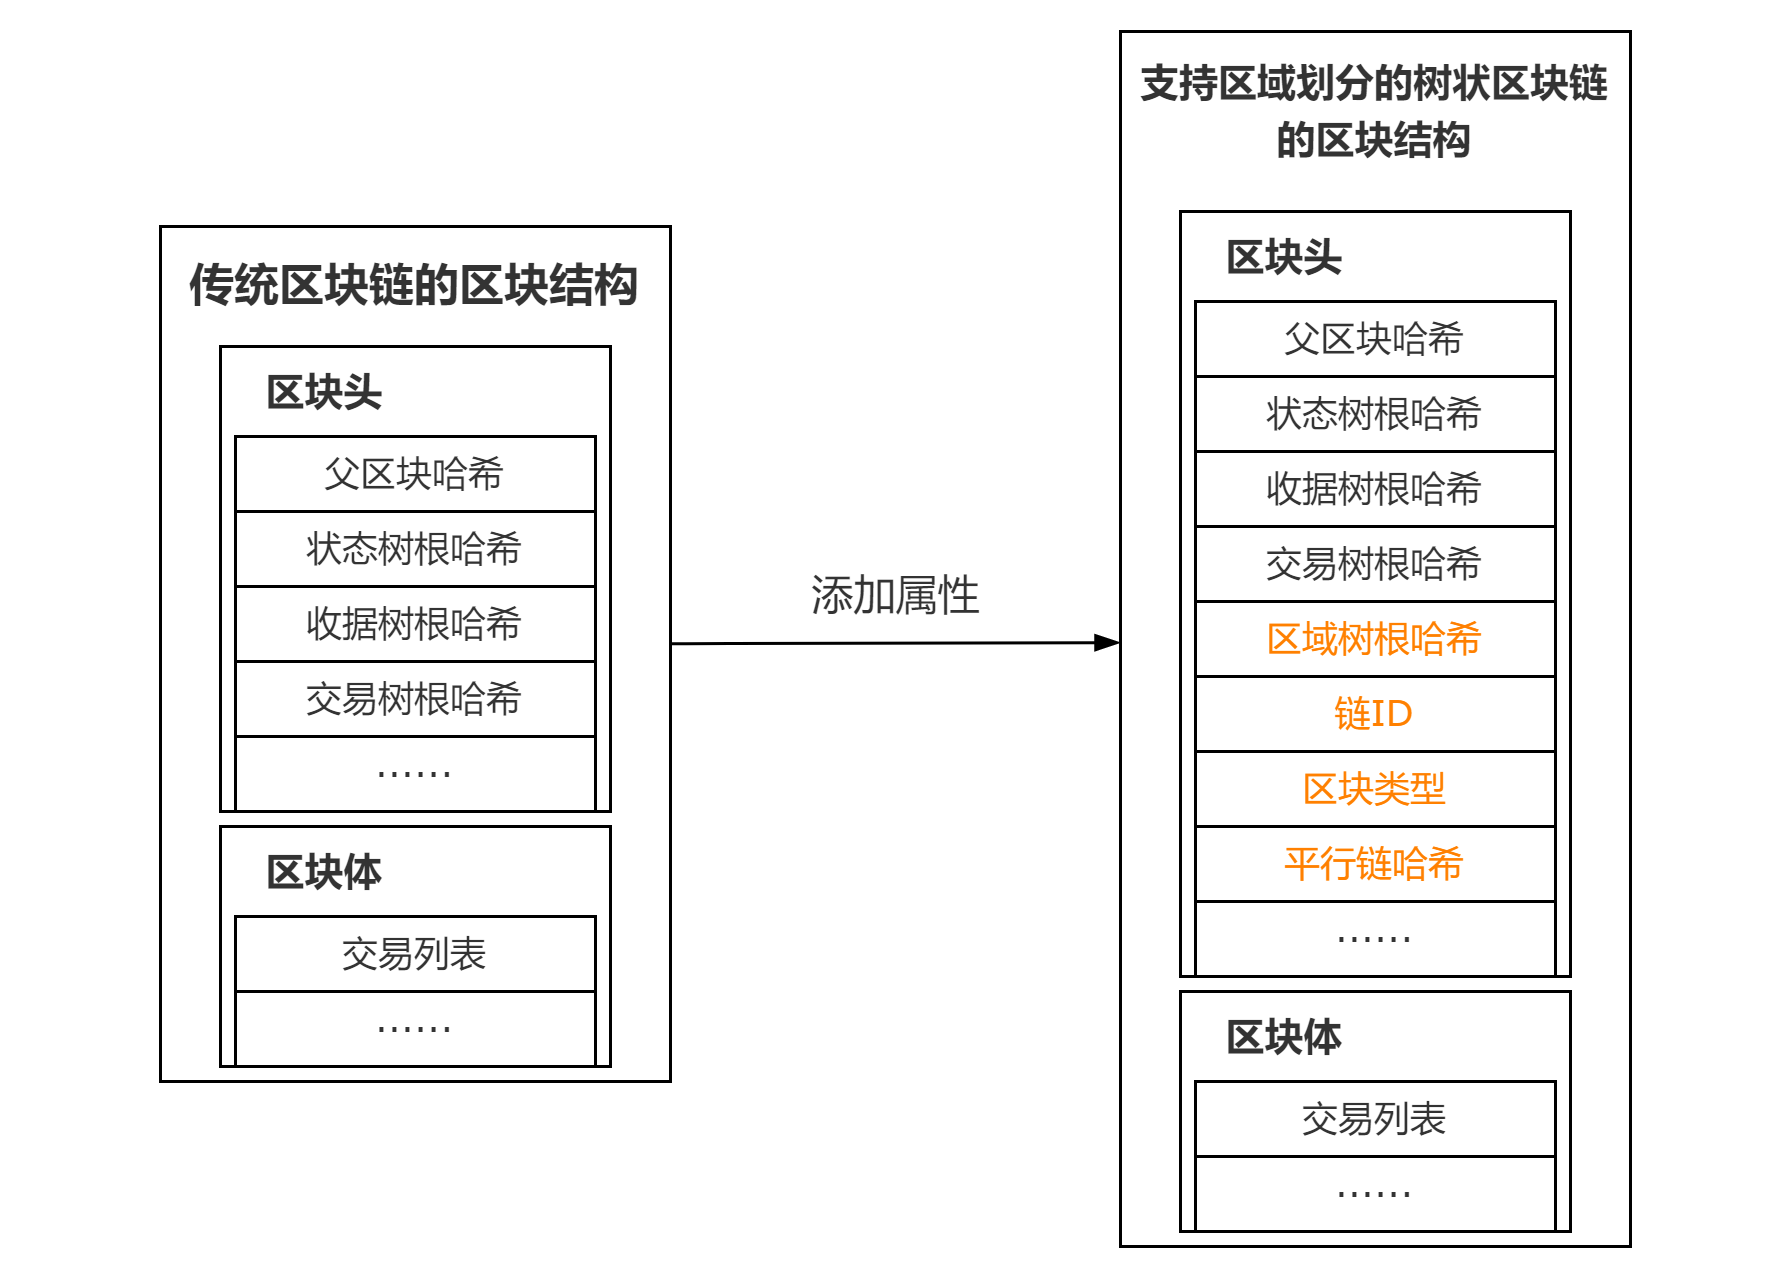
\includegraphics[width=0.8\textwidth]{undergraduate-thesis/images/TreeBlockchainNewProperty.png}
    \caption{支持区域划分的树状区块链结构示意图}
    \label{TreeBlockChain}
\end{figure}
% 结束放置单图片

\begin{enumerate}
    \item 按照Geohash编码的地理区域划分并更改区块数据结构。
    
    如图\ref{TreeBlockChain},相比于传统区块链,树状区块链在区块头中添加了同层块、块类型、链ID、区域根这四个属性。
    \begin{enumerate}
        \item 区域树根哈希:区域状态树(Region State Trie,RST)用于支持查询区域地理位置的相关数据。区域状态树用于记录地理区域内的全局变化,从而便于查询地理信息、验证数据可信。
        \item 链ID(chainID):用于区分来自不同区块链的区块。在多链的结构下,链ID一方面能方便按照不同子链同步区块内容,另一方面也能便利父链对子链的快速查询。
        \item 区块类型(blockType):支持区域划分的树状区块链结构有以下三类区块:创世块、分支区块、普通区块。该属性即对当前区块的类型进行区分。
        \item 平行链哈希(parallel Hash):分支区块用父链指针指向上层区块,用平行链指针指向跟自己拥有相同父区块、且Geohash编码位数相同的已产生的同层级分支区块。这样做便于使分支区块能维护其在树状区块链中的结构关系。
    \end{enumerate}
    \item 层次化分类区块与节点:
    \begin{enumerate}
        \item 区块分类:
        \begin{enumerate}
            \item 创世块:树状区块链结构里的第一个区块。全链的创世块保持一致。
            \item 分支区块:分支区域的第一个区块。在支持区域划分的树状区块链中,每增加一个层级,就增加32个分支区块。
            \item 普通区块:分支区域里的分支区块的子区块,记录对应地理区域内部发生的交易。
        \end{enumerate}
        \item 节点分类:
        \begin{enumerate}
            \item 全节点:维护全区块链完整的区块数据和全局状态树。部分服务器是全节点。
            \item 区域节点:维护其所在区域指定层次及以下的所有分支区块和普通区块。路侧节点和部分服务器是区域节点。
            \item 叶节点:是可以构建分支区块的最底层节点,维护其所在区域最下层的分支区块和普通区块。车辆节点是叶节点。
        \end{enumerate}
    \end{enumerate}
    \item 层次化组织区块:
    
    支持区域划分的树状区块链依据Geohash编码来完成层次化结构的组织。Geohash编码通过二分法将指定区域分为网格,每个网格的编码表示唯一。编码长度越长,则网格越小,对应的地区越精细,层次越低。根据Geohash编码的特性,该树状区块链的层次关系即对应地理区域的包含关系。因此,在该树状区块链中,上层分支区块对应的地理区域中,包含所有以该区块为父块的下层区块对应的地理区域。
    \item 区域信息汇总:

    在支持区域划分的树状区块链中,普通区块打包已发生的交易,分支区块提供子区块链的头区块和索引功能。当子链区块需要同步信息时,分支区块按照子链的地理区域独立进行区块汇总,将每个区域子链的待同步区块添加到分支区块链的对应分支上,并在分支节点处缓存汇总区域状态,以提高查询效率。
    
    支持区域划分的树状区块链融合地理位置,设计与地理位置相关的数据结构,通过Geohash的层级划分方式建立树状的多层级结构。将区块链以Geohash编码的方式,按照地理区域划分成多链,符合车辆节点在行驶过程中只对本区域地图数据感兴趣的特征,减少了每条链中的数据量和节点数量,提高了区块链的存储访问效率。
\end{enumerate}

\space 树状区块链融合地理位置,设计与地理位置相关的数据结构,通过Geohash的层级划分方式建立树状的多层级结构。将区块链以Geohash编码的方式,按照地理区域划分成多链,符合车辆节点在行驶过程中只对本区域地图数据感兴趣的特征,减少了每条链中的数据量和节点数量,提高了区块链的存储访问效率。

\subsection{复现树状区块链并部署合约}

树状区块链基于以太坊开发,其在以太坊底层区块链的基础上修改了数据结构,用go语言编译为新的geth客户端。本节将对支持区域划分的树状区块链进行复现,并在其上完成合约部署。

具体的复现手册地址见附录D。

复现部署树状区块链的过程主要经历以下环节:利用genesis.json文件初始化并启动区块链,新建账户并给账户添加余额,再次初始化区块链,确保账户中余额添加成功。在该过程中,主要需关注如下问题:

\begin{comment}
\begin{figure}[ht]
    \centering
    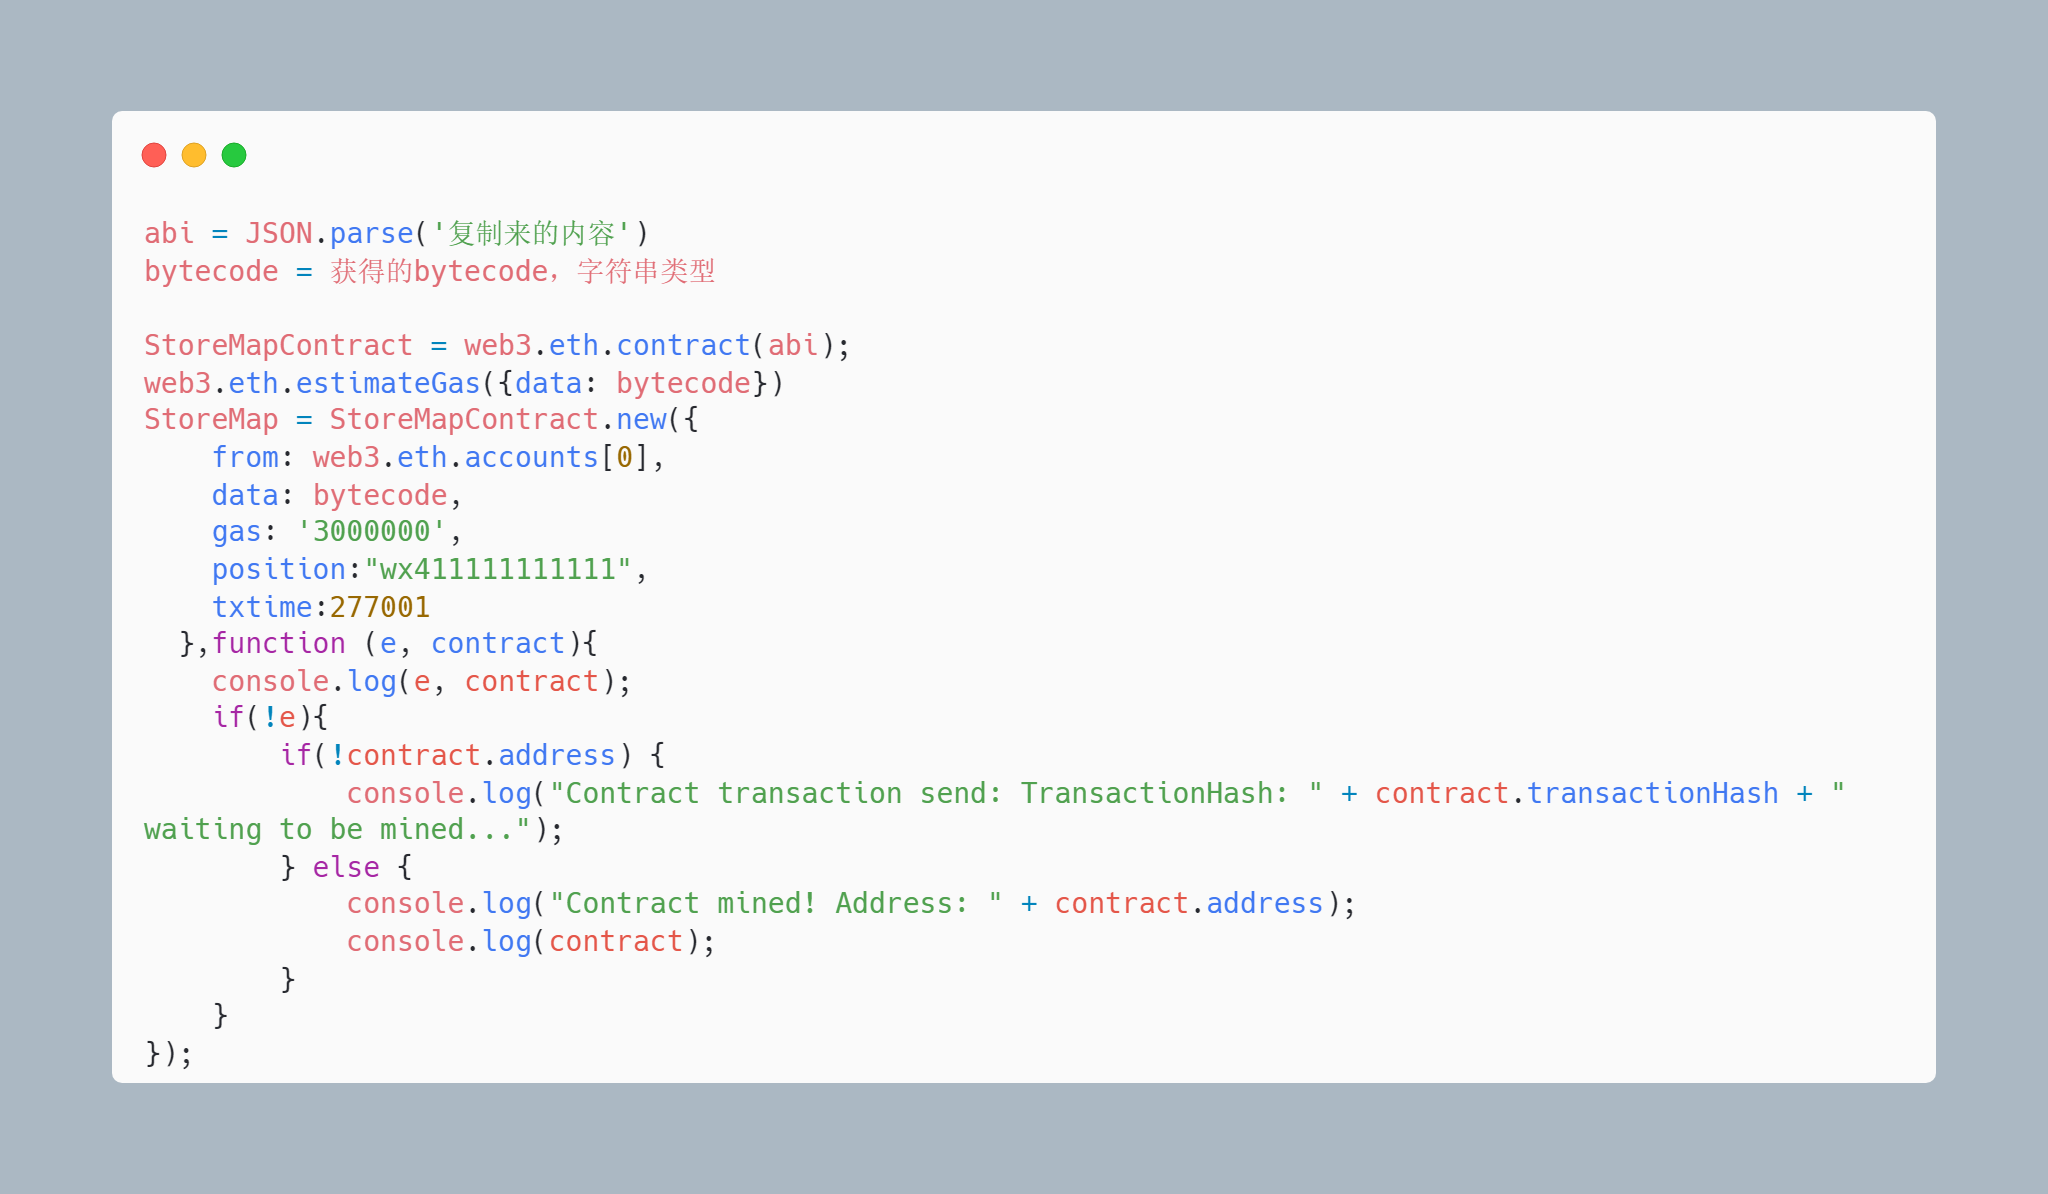
\includegraphics[width=0.7\textwidth]{undergraduate-thesis/images/ContractUpload.png}
    \caption{以StoreMap.sol合约为例的部署代码}
    \label{ContractUpLoad}
\end{figure}
\end{comment}

\begin{enumerate}
    \item 每次重新打开区块链,都需要再解锁一次账户,否则miner.start()无法挖到合约地址。
\begin{lstlisting}[language=java, caption={解锁账户}, label={lst:unlockAccounts}]
    for (i = 0; i < eth.accounts.length; i++) { personal.unlockAccount(eth.accounts[i],"123456",0) }\end{lstlisting}
    \item 在部署合约时,需要格外关注代码2.2中所示的position字段,其需以初始化、启动区块链时,操作语句中的networkid为前缀,否则无法部署到对应树状区块链中。
\begin{lstlisting}[language=java, caption={StoreMap.sol的合约部署代码节选}, label={lst:uploadContract}]
StoreMap = StoreMapContract.new({
    from: web3.eth.accounts[0], 
    data: bytecode, 
    gas: '3000000',
    position:"wx411111111111",
    txtime:277001
},function (e, contract){ }\end{lstlisting}
    
\end{enumerate}

\subsection{复现出租车调度系统}
复现出租车调度系统的过程主要经历以下环节:上传地图、修改脚本里的合约地址和账户名称信息、打开网页接口、启动测试脚本。

具体的复现手册地址见附录D。

在复现过程中,主要需要关注的问题在打开区块链和网页接口部分:

\begin{enumerate}
    \item 首先,要确保区块链的外部访问接口和网络的外部访问接口都已被打开,使用以下语句初始化、启动区块链:
\begin{lstlisting}[language=bash, caption={初始化、启动区块链}, label={lst:initBlockChain}]
    // 初始化区块链
    geth1 --identity "MyEth" --rpc --rpcaddr 0.0.0.0  --rpcport "8545" --rpccorsdomain "*" --datadir gethdata --port "30303" --nodiscover --rpcapi "eth,net,personal,web3" --networkid 91036 init genesis.json
    // 启动区块链
    geth1 --datadir ./gethdata --networkid 91036 --port 30303 --rpc --rpcaddr 0.0.0.0 --rpcport 8545 --rpcapi 'personal,net,eth,web3,admin' --rpccorsdomain='*' --ws --wsaddr 0.0.0.0 --wsport 8546 --wsorigins='*' --wsapi 'personal,net,eth,web3,admin' --nodiscover --allow-insecure-unlock --dev.period 1 --syncmode='full' console\end{lstlisting}
    相比于本地区块链来说,在初始化和启动可被多设备访问的区块链时,需要把代码中的 rpcaddr 127.0.0.1 和 wsaddr=`localhost'修改为 rpcaddr 0.0.0.0 和 wsaddr 0.0.0.0。这样做的目的是为了便于跨设备访问出租车调度系统,否则区块链只被部署在本地,无法被外部机器访问,就无法用其余设备完成对区块链的访问。
    
    \item 在实际的出租车调度系统中,需要修改网络接口:
    \begin{enumerate}
        \item 从虚拟机的终端中获取虚拟机的IP。
\begin{lstlisting}[language=bash, caption={获取虚拟机IP}, label={lst:getIP}]
    hostname -I\end{lstlisting}
        \item 将config/index.js中的host改为0.0.0.0。
\begin{lstlisting}[language=bash, caption={修改config/index.js}, label={lst:fixindex}]
    host: '0.0.0.0', // can be overwritten by process.env.HOST
    port: 8081, // can be overwritten by process.env.PORT, if port is in use, a free one will be determined\end{lstlisting}
        \item 修改Global.vue中的全局配置,在``ws://"后接入(a)中查询所得的当前虚拟机所在IP。
        \begin{lstlisting}[language=html, caption={修改Global.vue}, label={lst:changeIP}]
this.web3Map = new Web3(
    //new Web3.providers.WebsocketProvider("ws://127.0.0.1:8546")
    new Web3.providers.WebsocketProvider("ws://IP:8546")
);\end{lstlisting}
    \end{enumerate}
\end{enumerate}

\section{真实地图数据准备}

\space 出租车调度系统的运行需要基于北京市的真实地图,因此,本文给出了一种获取并处理真实地图数据、并将其上传给支持区域划分的树状区块链的方法。本节将对该方法进行描述。

\subsection{地图数据描述}
本文采用的真实地图路网源数据位于北京市内,由Geofabrik提供。数据格式为shp格式,为截至2023年4月13日的最新路网数据。本文利用ArcGIS软件按照北京的经纬度范围,从全国路网数据中裁剪出了位于经度(116.027390,116.780607)、纬度(39.688683,40.168784)范围的路网数据,其将北京的主要区域均包含在内。本文在在此基础上对该数据进行处理。

% 设置三线表
\begin{table}[ht]
    \linespread{1.5}
    \zihao{5}
    \centering
    \caption{shp格式路网数据的主要基本属性}
    \label{mapDataProperty}
    \begin{tabular}{cccc}
    \toprule
    字段名称 & 注释 & 类型 & 示例     \\ 
    \hline
    gid & 路网表的主码列 & integer & 17576 \\
    osm\_id & 标识道路的osm序号 & character varying(12) & ``554383619" \\
    code & 标识道路类型 & smallint & 5122 \\
    fclass & 标识道路类型 & character varying(28) & ``tertiary" \\
    name & 记录道路名称 & character varying(100) & ``兴贸南街" \\
    oneway & 标识道路是否为单行道 & character varying(1) & ``B" \\
    bridge & 标识道路是否为桥梁 & character varying(1) & ``F" \\
    tunnel & 标识道路是否为隧道 & character varying(1) & ``F" \\ 
    gemo & 路网表中包含的空间信息 & geometry & \makecell{``010100002031BF0\\D00E17A14969BA5684\\1F6285C2FBE815241"} \\
    \bottomrule
    \end{tabular}
\end{table}
% 结束设置三线表
路网数据主要的基本属性如表\ref{mapDataProperty}所示。

根据Geohash编码特性,为了获取同处一个Geohash编码区域的所有车辆可同行的路网数据,本文筛选了如图\ref{mapDataRegion-big}所示的四个区块,并估算其经纬度,在数据库中完成筛选。

\begin{figure}[ht]
    \centering
    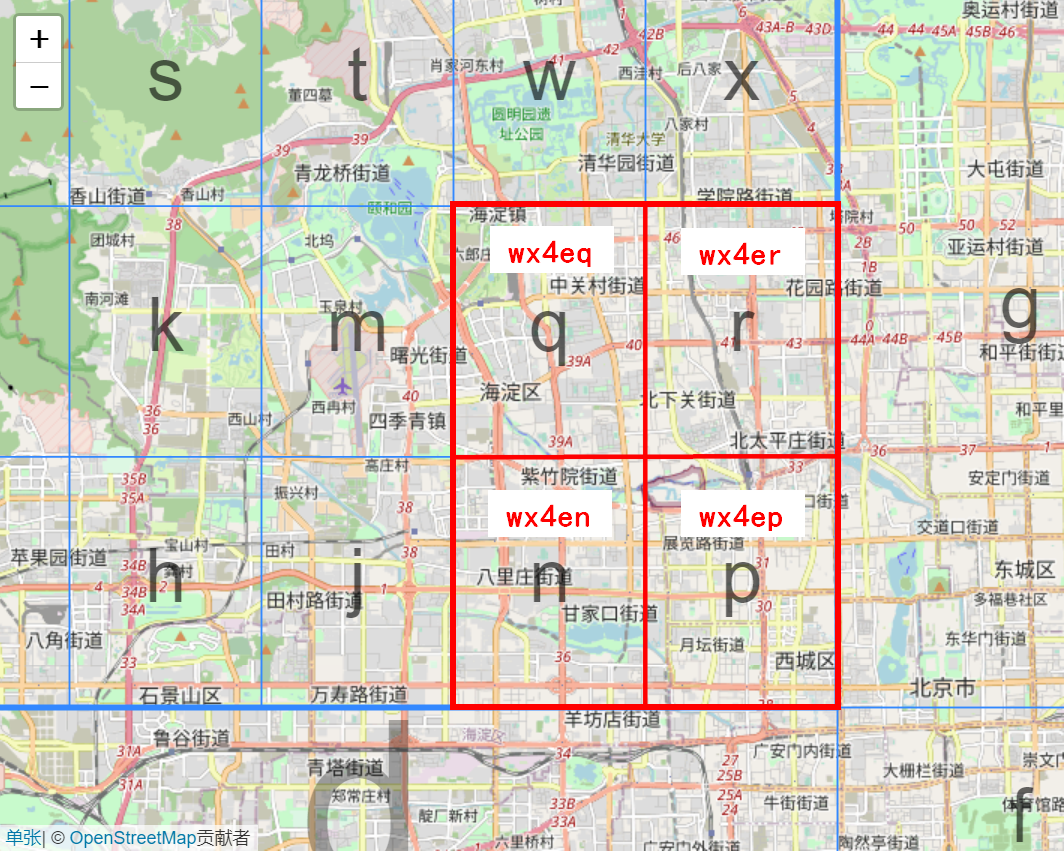
\includegraphics[width=0.6\textwidth]{undergraduate-thesis/images/FourRegions.png}
    \caption{以wx4e为前缀的四个五位编码区块示意图}
    \label{mapDataRegion-big}
\end{figure}

这四个区块对应的经纬度如表\ref{mapDataRegion-number}所示:

% 设置三线表
\begin{table}[ht]
    \linespread{1.5}
    \zihao{5}
    \centering
    \caption{区域经纬度范围}
    \label{mapDataRegion-number}
    \begin{tabular}{ccc}
    \toprule
    % \Xhline{1.5pt}
    区块的Geohash编码 & 经度范围 & 纬度范围 \\
    \midrule
    % \Xhline{0.5pt}  
    wx4eq & [116.279,116.323] & [39.947,39.991]\\
    wx4er & [116.323,116.367] & [39.947,39.991]\\
    wx4en & [116.279,116.323] & [39.903,39.947]\\
    wx4ep & [116.323,116.367] & [39.903,39.947]\\
    \bottomrule
    %\Xhline{1.5pt}
    \end{tabular}
\end{table}
% 结束设置三线表

\subsection{地图数据处理}

本文在处理地图数据时,主要采用地理信息处理软件ArcGIS和地理空间数据库PostgreSQL,具体涉及到的软件、插件及对应版本如表\ref{mapDataApp}所示:
\begin{table}[ht]
    \linespread{1.5}
    \zihao{5}
    \centering
    \caption{处理真实地图数据需要的软件、插件列表}
    \label{mapDataApp}
    \begin{tabular}{cc}
    \toprule
    % \Xhline{1.5pt}
    软件、插件名称 & 版本 \\
    \midrule
    % \Xhline{0.5pt}  
    ArcGIS & 10.8\\
    ArcGIS Editor for OSM & 10.8\\
    PostgreSQL & 6.21\\
    PostGIS & 3.3.2\\
    pgRouting & 3.4.2\\
    \bottomrule
    %\Xhline{1.5pt}
    \end{tabular}
\end{table}

使用以上工具处理地图数据时,需要经历以下步骤:用ArcGIS处理数据、用PostgreSQL处理数据、用脚本编码数据、向区块链上传数据。

1.用ArcGIS处理数据:

(a)数据裁剪:删去其他省市数据,缩减地图范围集中在北京区域,方便后续处理。

(b)要素转线:以两条道路的交叉点为基础打断道路,实现道路的分段效果。

(c)获取每个路段两端的经纬度:提前在ArcGIS中获取路段两端的经纬度数据,以便在PostgreSQL中直接筛选。

2.用PostgreSQL处理数据:

(a)导入数据库:将经由ArcGIS处理过的shp格式文件,以WGS84坐标系(SRID=4326)的投影方式导入数据库中。

(b)计算道路距离:在PostgreSQL中计算道路成本,并根据道路成本和道路经纬度建立路网拓扑回路。

(c)导出数据:在完成以上步骤中,PostgreSQL中应有如表\ref{mapData_Addproperty}中所示的新增项。然后在路网表中用SQL语句将所有筛选出的数据转为单行的Json语句,导出为一个Json文件。

3.用脚本编码数据:用JavaScript脚本处理导出的Json文件,主要是对每个路段的经纬度进行Geohash编码,形成一个包含Geohash编码信息的Json文件。

4.向区块链上传数据:将含有Geohash编码信息的Json文件上传给支持区域划分的树状区块链。该数据文件所在的Github仓库地址见附录D。

\begin{table}[ht]
    \linespread{1.5}
    \zihao{5}
    \centering
    \caption{从数据库中导出地图数据时必要的字段}
    \label{mapData_Addproperty}
    \begin{tabular}{cccc}
    \toprule
    % \Xhline{1.5pt}
    字段名称 & 注释 & 类型 & 示例\\
    \midrule
    % \Xhline{0.5pt}  
    start\_x & 该路段起始点经度 & numeric & 116.331388100 \\
    start\_y & 该路段起始点纬度 & numeric & 39.7695126000 \\
    end\_x & 该路段终止点经度 & numeric & 116.332542000 \\
    end\_y & 该路段终止点纬度 & numeric & 39.7695167000 \\
    cost & 道路的正向成本(代价) & double precision & 659.8882769759143 \\
    reverse\_cost & 道路的逆向成本(代价) & double precision & 659.8882769759143 \\
    source & 保存路径起始顶点的id(上一段道路) & integer & 830 \\
    target & 保存路径终止顶点的id(下一段道路) & integer & 835 \\
    \bottomrule
    %\Xhline{1.5pt}
    \end{tabular}
\end{table}

本章中使用的SQL查询语句见附录B。通过该语句导出的地图,包含了表\ref{mapData_pathpro}类型的道路数据:

\begin{table}[ht]
    \linespread{1.5}
    \zihao{5}
    \centering
    \caption{本文筛选的道路类型}
    \label{mapData_pathpro}
    \begin{tabular}{cccc}
    \toprule
    % \Xhline{1.5pt}
    道路等级 & \makecell{数据库中\\fclass字段值} & \makecell{数据库中\\code字段值} & 描述 \\
    \midrule
    % \Xhline{0.5pt}  
    国道、城市快速路 & trunk & 5112 & \makecell{城市道路系统中的快速路,\\重要性次于高速公路的公路。}\\
    省道、主干道 & primary & 5113 & \makecell{连接主要区域、城镇的道路,\\城市内较重要的市政道路。 }\\
    县道、次干道 & secondary & 5114 & \makecell{连接主要区域、村镇但不及省道的道路,\\城市道路系统中的次干道。} \\
    乡道、支路 & tertiary & 5115 & \makecell{连接村与村的道路,\\市政道路中狭窄的双向、单向2车道。}\\
    国道匝道 & trunk\_link & 5132 & 连接国道/快速路、更低级道路的连接路。\\
    省道匝道 & primary\_link & 5133 & 连接省道/主干道、更低级道路的连接路。\\
    县道匝道 & secondary\_link & 5134 & 连接县道/次干道、更低级道路的连接路。\\
    乡道匝道 & tertiary\_link & 5135 & 连接乡道/支路、更低级道路的连接路。\\
    \bottomrule
    %\Xhline{1.5pt}
    \end{tabular}
\end{table}

\section{本章小结}

本章聚焦于研究工作的数据部分,首先介绍了周畅的支持区域划分的树状区块链的设计方式,其次介绍了对实验室前人工作的复现过程,最后介绍了地图数据的获取和处理流程,为后续在实验室已有工作的基础上开展基于实时路况的A*算法的设计与测试打下了良好的基础。
\chapter{基于实时路况的调度系统设计}

本章首先介绍了基于区块链的出租车调度系统结构,然后介绍了传统A*算法的工作原理,并在此基础上结合实时路况,提出了一种改进后的A*算法,最后将改进后的A*算法与出租车调度系统融合,形成一个基于实时路况的出租车调度系统。
% 第三章的开头加一节,展现整个系统的结构,包括系统组成部分,各部分的相互关系和接口。

\section{基于区块链的调度系统结构分析}

\begin{figure}[ht]
  \centering
  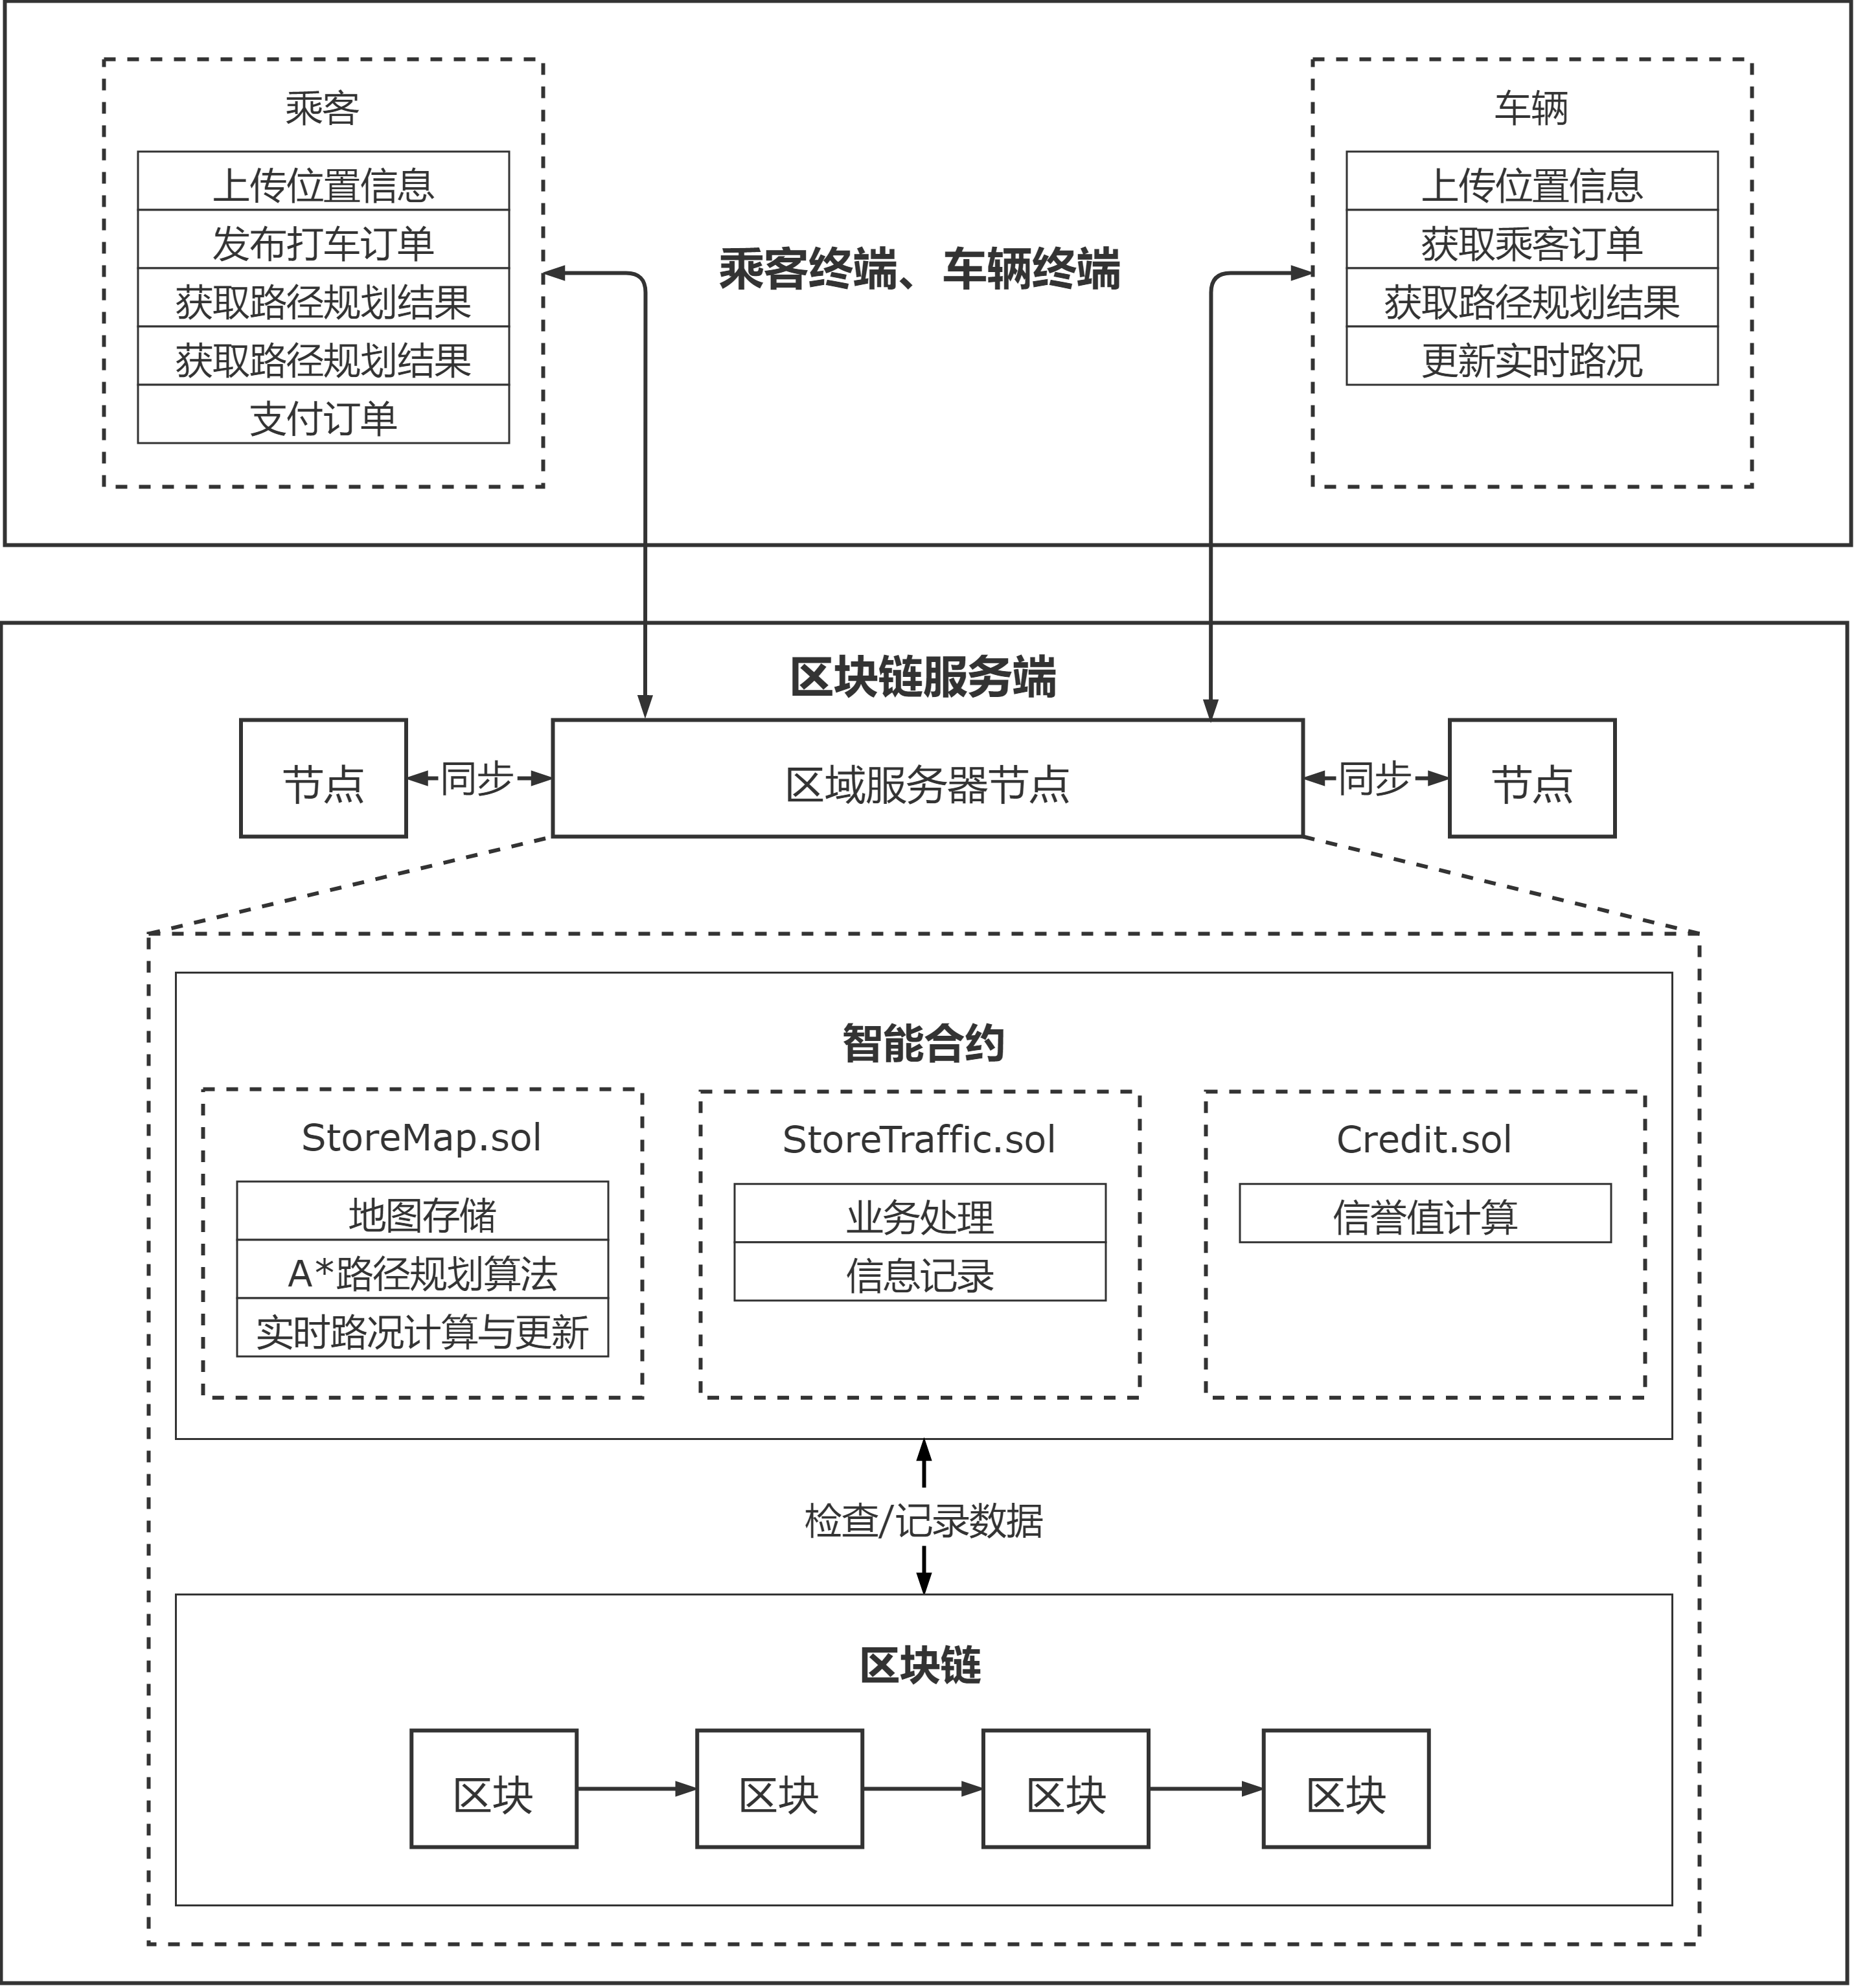
\includegraphics[width=0.7\textwidth]{undergraduate-thesis/images/sysstructure.png}
  \caption{基于区块链的出租车调度系统结构}
  \label{pic-sysstructure} % label 用来在文中索引
\end{figure}

图\ref{pic-sysstructure}是基于区块链的出租车调度系统结构示意图。本系统主要分为区块链服务器端和终端两部分,其中终端包括乘客终端与车辆终端。本系统去中心化,且为了保证身份信息的匿名性,乘客终端与车辆终端分别只与区块链交互,从而保证车乘之间不产生直接的信息交互。

\subsection{区块链服务器端}

区块链服务器端主要分区块链和智能合约两部分。

区块链部分主要实现数据存储功能,其存储交易相关数据与系统运行的地图数据。将数据存储在区块链上,能利用区块链数据的不可篡改性,保证交易安全有效,被需要时可以及时完成溯源。同时,当终端与区块链进行信息交互时,区域服务器节点也会与其他节点进行同步记录,保证在单个节点出问题时,其他节点能正常运行,而不受问题节点的影响,从而保证了数据的安全性。

智能合约部分主要负责对数据进行处理,它将区块链的功能从简单的记账拓展为复杂的事件响应、数据处理。本系统中共设计三个智能合约,其按功能被划分为地图合约(StoreMap.sol)、交通合约(StoreTraffic.sol)、信誉值合约(Credit.sol)。本文对地图合约进行了功能上的完善,为其补充了实时路况计算模块、并因此对地图合约里的A*算法进行了修改。下文将分别介绍这三个合约的功能。

1.地图合约主要完成地图存储、A*路径规划算法、实时路况计算与更新功能。该合约首先与地图上传脚本进行交互,将Geohash编码后的Json格式地图数据部署到区块链上,实现地图存储的功能。接下来,在终端的运行过程中,该合约根据终端发出的不同请求完成以下流程:在区块链上存储乘客、车辆位置信息;获取乘客的打车订单并运行车乘匹配算法为该订单调度车辆;将匹配结果告知乘客与车辆;为车辆规划出接乘客的路径并把结果返回给终端;为车辆规划出送乘客到目的地的路径并把结果返回给终端;根据送乘客的路径规划结果更新实时路况,并在区块链中以存储道路属性数据的形式存储路况。

2.交通合约主要完成业务处理、信息记录功能。在业务处理功能中,交通合约通过接收乘客的打车请求,实现按区域的车乘匹配,当车辆接到订单并选择接客后,交通合约修改车辆与乘客的状态为已载客、已乘车。信息记录功能则主要是对信息的处理过程,其接收到终端发来的车乘的位置信息、账户信息,同时也能修改车辆与乘客的载客与乘车状态,还能将乘客的支付状态告知给车辆,并且支持车辆退出系统的效果。

3.信誉值合约主要完成对车辆信誉值的计算。该合约把司机活跃度、车辆位置验证结果、车辆接单率、乘客主观评分四方面作为影响因子,进行计算,给出车辆的信誉值数据,使信誉值计算能综合车辆位置验证与交易评价两方面因素,更加全面合理。

\subsection{终端}

终端主要分为车辆终端与乘客终端。终端的实现方式分为脚本实现与浏览器实现。脚本实现方式的运行时间较浏览器实现更短。但浏览器实现能可视化观察到,在系统运行的各环节中,地图信息、车辆与乘客的位置、规划出的路径信息。本文工作重点为基于实时路况对A*算法进行改进,通过浏览器实现能更加直观给出本工作所得的动态路径规划效果,因此,本文主要通过浏览器实现的方式完成车辆终端与乘客终端的运行。

1.车辆终端通过web3接口与区块链服务端进行数据的交互,这些数据包括:在前端用于展示的地图数据、可视化的位置与路径规划结果信息数据;向区块链服务端发送自己的位置、账户信息,发送自己是否接客的信息;向区块链服务端发送信息,用于调用路径规划、实时路况计算等过程;从区块链服务端中获取打车订单信息,获取乘客支付信息。

2.乘客终端通过web3接口与区块链服务端进行数据的交互,这些数据包括:在前端用于展示的地图数据、可视化的位置与路径规划结果信息数据;向区块链服务端发送自己的位置、账户信息,发布打车订单,发送支付完成的信息;从区块链服务端中获取接到订单的车辆信息。

\section{传统A*算法与实时路况}

\subsection{传统A*算法的工作原理}
\label{A*Reason}

A*算法是一种在静态的路网中求解最短路径的直接搜索方法。该算法将Dijkstra算法和广度优先算法相结合,利用启发式函数寻找距起点代价最小的终点,从而规划出一条最短路径。该算法常被用于在地图中进行全局路径规划,也常常用于游戏中虚拟角色的移动计算。

A*算法将区域划分为小格,每个小格代表一个节点。A*算法以起点为中心,辐射性搜索周围的邻居节点,并计算每个节点的总距离代价,寻找代价最小的点继续移动,直至寻找到终点。针对节点n,A*算法将耗散函数、启发函数同时整合进公式\ref{cal-Astar}中,计算该节点的距离代价。
\begin{equation}
    F(n)=G(n)+H(n)
\label{cal-Astar}
\end{equation}

F(n)代表节点n对应的总距离代价;G(n)是耗散函数,它代表从起点到节点n,该路径已经花费掉的所有代价,也即从起点到节点n的实际距离;H(n)是启发函数,它代表从节点n到终点,预估将要花费的代价。

对第n个节点来说,由于耗散函数G(n)代表它从起点到该点的实际距离,因此G(n)的值一般为固定值,它的计算方式也是固定的。启发函数H(n)的选取方式则相对多样。在A*算法中,启发函数的选取也是至关重要的一环。启发函数的作用是预估从节点n到终点所需的距离代价。

在公式\ref{cal-Astar}中,如果令H(n)=0,则F(n)=G(n),此时总距离代价完全由耗散函数G(n)控制,则A*算法将退化为Dijkstra算法。在这种情况下,尽管最终仍能寻到起点与终点之间的最短路径,但消耗的时间和内存空间都将较H(n)≠0时有所增加。

在公式\ref{cal-Astar}中,如果令G(n)=0,则F(n)=H(n),此时总距离代价完全由启发函数H(n)控制,则A*算法将退化为广度优先搜索。这种情况将导致算法进行盲目的搜寻,其不注重结果的可能位置,而是彻底搜索整个图,尽管它也能给出规划结果,但它找出的结果是单一的,有时甚至找不到最短路径,且消耗的时间和内存空间也较G(n)≠0时更多。

因此,给G(n)和H(n)分配适当的权值,从而令A*算法有一个合适的评估函数F(n),是非常关键的。一般在计算时给G(n)和H(n)分配的比例是1:1,本文中也沿用此评估函数。

在计算启发函数H(n)时,常常有以下几种计算方法:

\begin{enumerate}
    \item 欧几里得距离(Euclidean distance):
        \begin{equation}
            D(M,N)=\sqrt[2]{ (x_{2}-x_{1})^{2} + (y_{2}-y_{1})^{2}} 
        \label{Eu-dis}
        \end{equation}

        欧几里得距离也称欧氏距离。假设待计算的两点坐标为:M(x1,y1)、N(x2,y2),则该计算方式得出的结果D(M,N)是两个地理位置之间的直线距离,如公式\ref{Eu-dis}。
        
        该距离计算公式适用于能朝任何方向移动的路径规划过程。
    
    \item 曼哈顿距离(Manhattan Distance):
        \begin{equation}
            D(M,N)=\left | x_2-x_1 \right | + \left | y_2-y_1 \right |
            \label{Man-dis}
        \end{equation}
        
        假设待计算的两点坐标为M(x1,y1)、N(x2,y2),则该计算方式得出的结果D(M,N)是两个地理位置在标准坐标系上的绝对轴距总和,如公式\ref{Man-dis}。

        该距离公式适用于能朝上下左右四个方向移动的路径规划过程。
\end{enumerate}

% 空行有点点大惹,看看怎么减一减
% \vspace{-1cm}
\begin{figure}[ht]
  \centering
  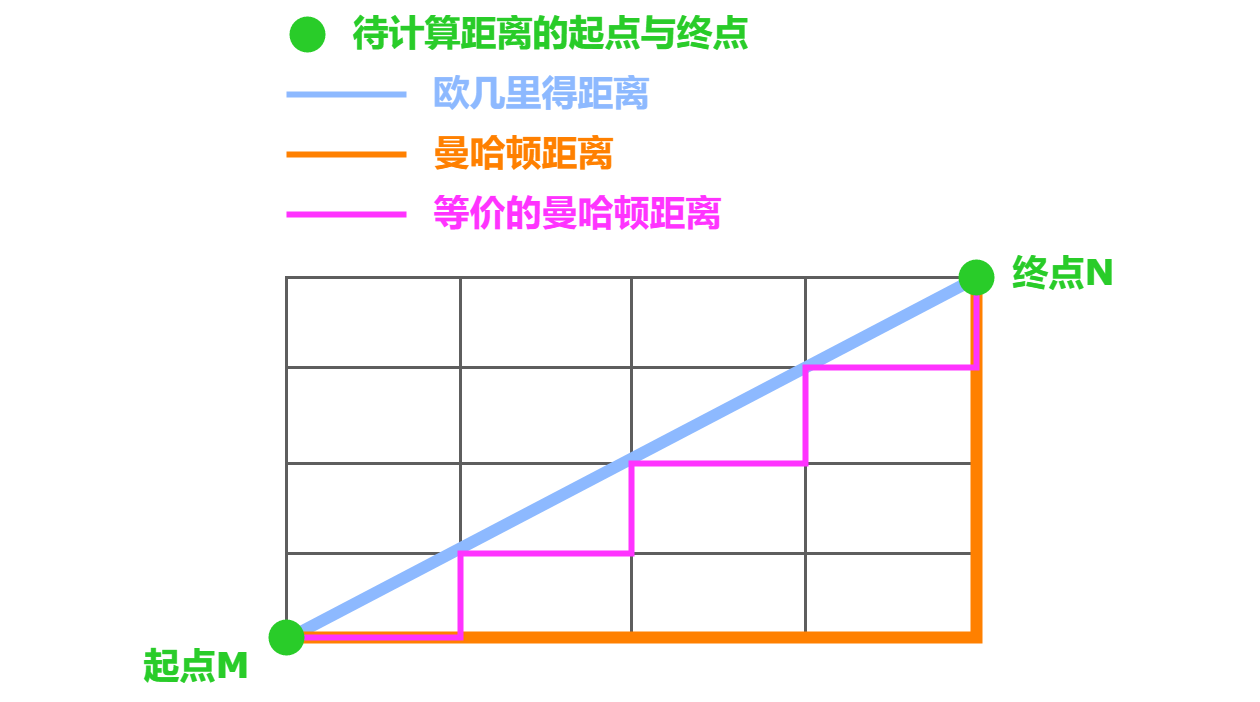
\includegraphics[width=0.5\textwidth]{undergraduate-thesis/images/EuDis_and_ManDis.png}
  \caption{欧几里得距离和曼哈顿距离示意图}
  \label{EuDisAndManDis} % label 用来在文中索引
\end{figure}

以一个3*4大小的方格区域为例,在该方格区域中分别使用这两种距离计算方法计算起点与终点间的距离,其各自规划出的路径如图\ref{EuDisAndManDis}所示。可以看到,用欧几里得距离规划路径时,由于欧几里得距离允许车辆向任何方式行驶,所以它直接按照蓝色斜线从起点前往终点;用曼哈顿距离规划路径时,它将按照方格边缘行驶,即只沿正南、正北、正东、正西方向计算路程,最终按照橙色折线或粉色折线从起点前往终点。

由于城市中的道路大多具有固定朝向,不存在行驶中的车辆能朝着任意方向运行的可能性。且在基于Geohash编码地图时,会将地图划分成不同区域的小方格,符合曼哈顿距离在计算时的沿方格边沿计算特性,因此在本出租车调度系统中,采取曼哈顿距离作为A*算法中的启发函数。

\begin{figure}[ht]
  \centering
  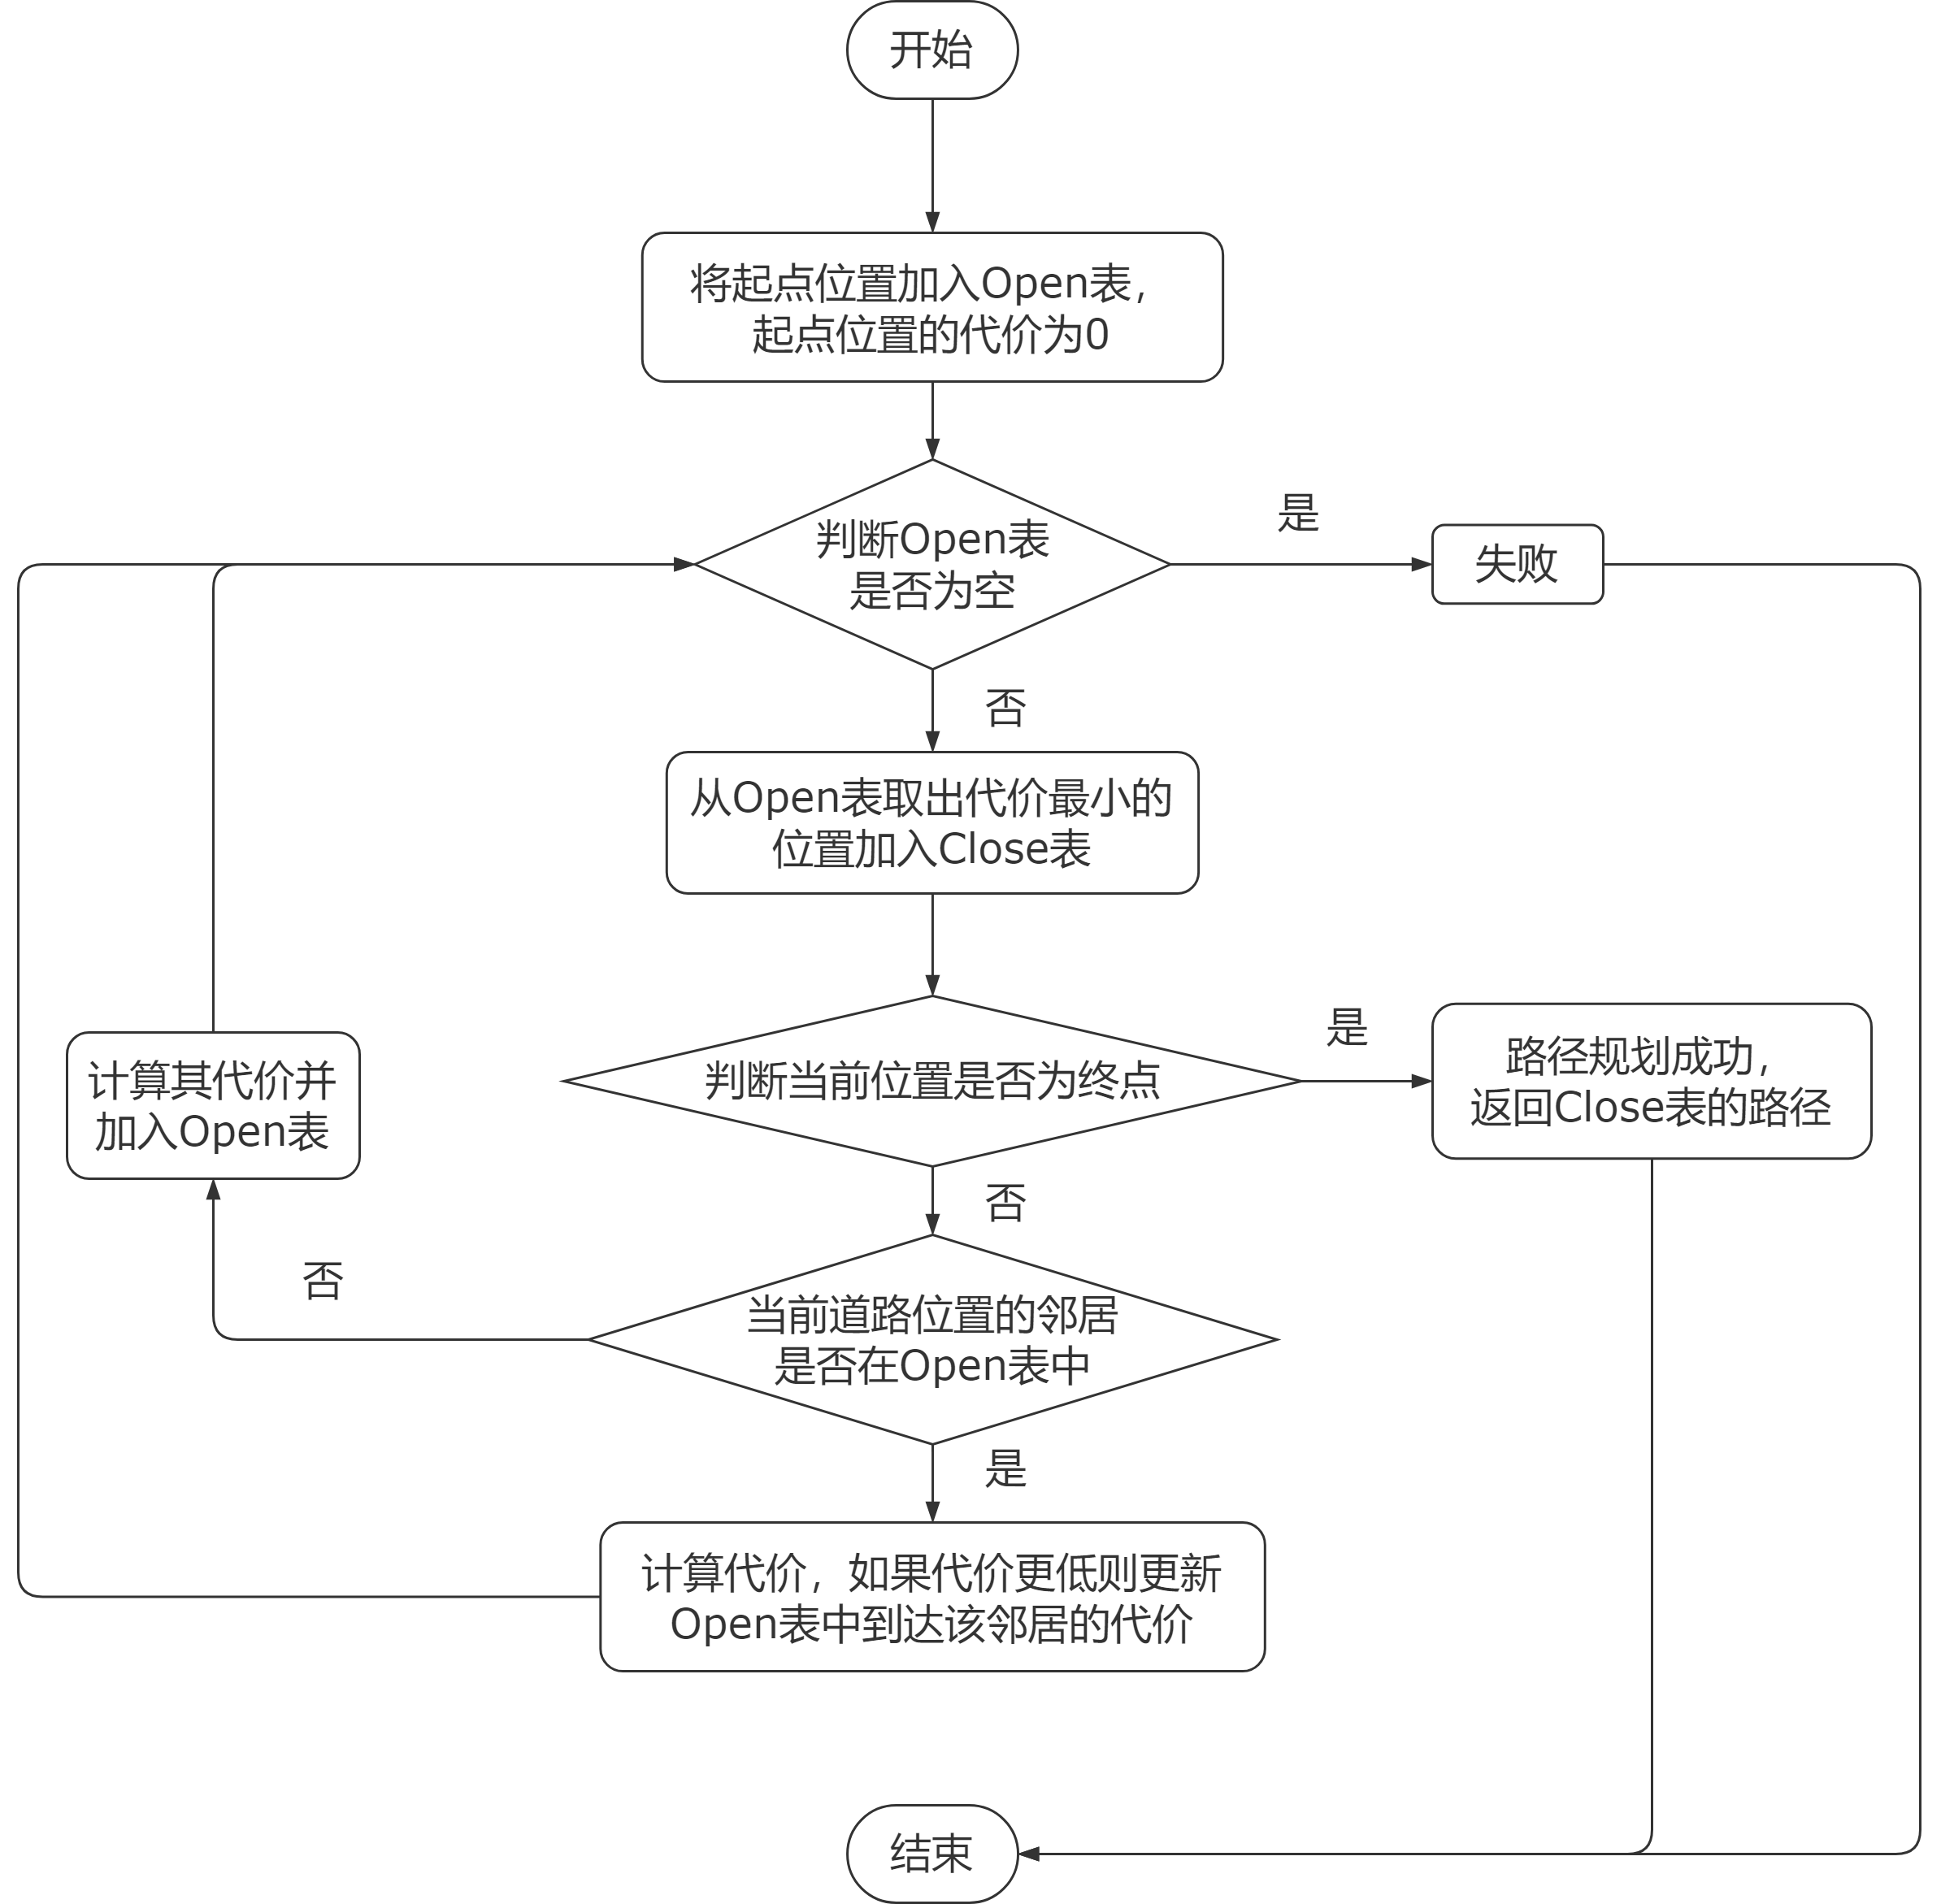
\includegraphics[width=0.65\textwidth]{undergraduate-thesis/images/Astar_Workway.png}
  \caption{A*算法流程图}
  \label{AstarWorkWay} % label 用来在文中索引
\end{figure}

如图\ref{AstarWorkWay}所示,A*算法在运行时的关键在于维护Open表和Close表、计算总距离代价F。设当前节点为P,则P点的每一个邻居$p_i$都存在其总距离代价F($p_i$)。Open表中记录所有与P相邻的点,它集中了节点P有可能前往的所有下一个节点;Close表中记录已走过的点,它集中了目前的路径规划已走过的道路,这意味着Close表中的点一定是最终规划出的最短路径中会经过的点。对节点P来说,计算完它邻居$p_i$的总距离代价F($p_i$)后,从所有的F($p_i$)中找到最小值F($p_{min}$)及其对应的点P$_{min}$点,将P$_{min}$点加入Close表中,然后把当前节点P移至节点P$_{min}$,再去计算P$_{min}$点的邻居的总距离代价F,从而从起点一层层向外扩散移动,直至寻找到终点。一旦A*算法寻找到终点,Close表中存放的点序列就是此次算法运行所规划好的运行路径。

\begin{figure}[!ht]
  \centering
  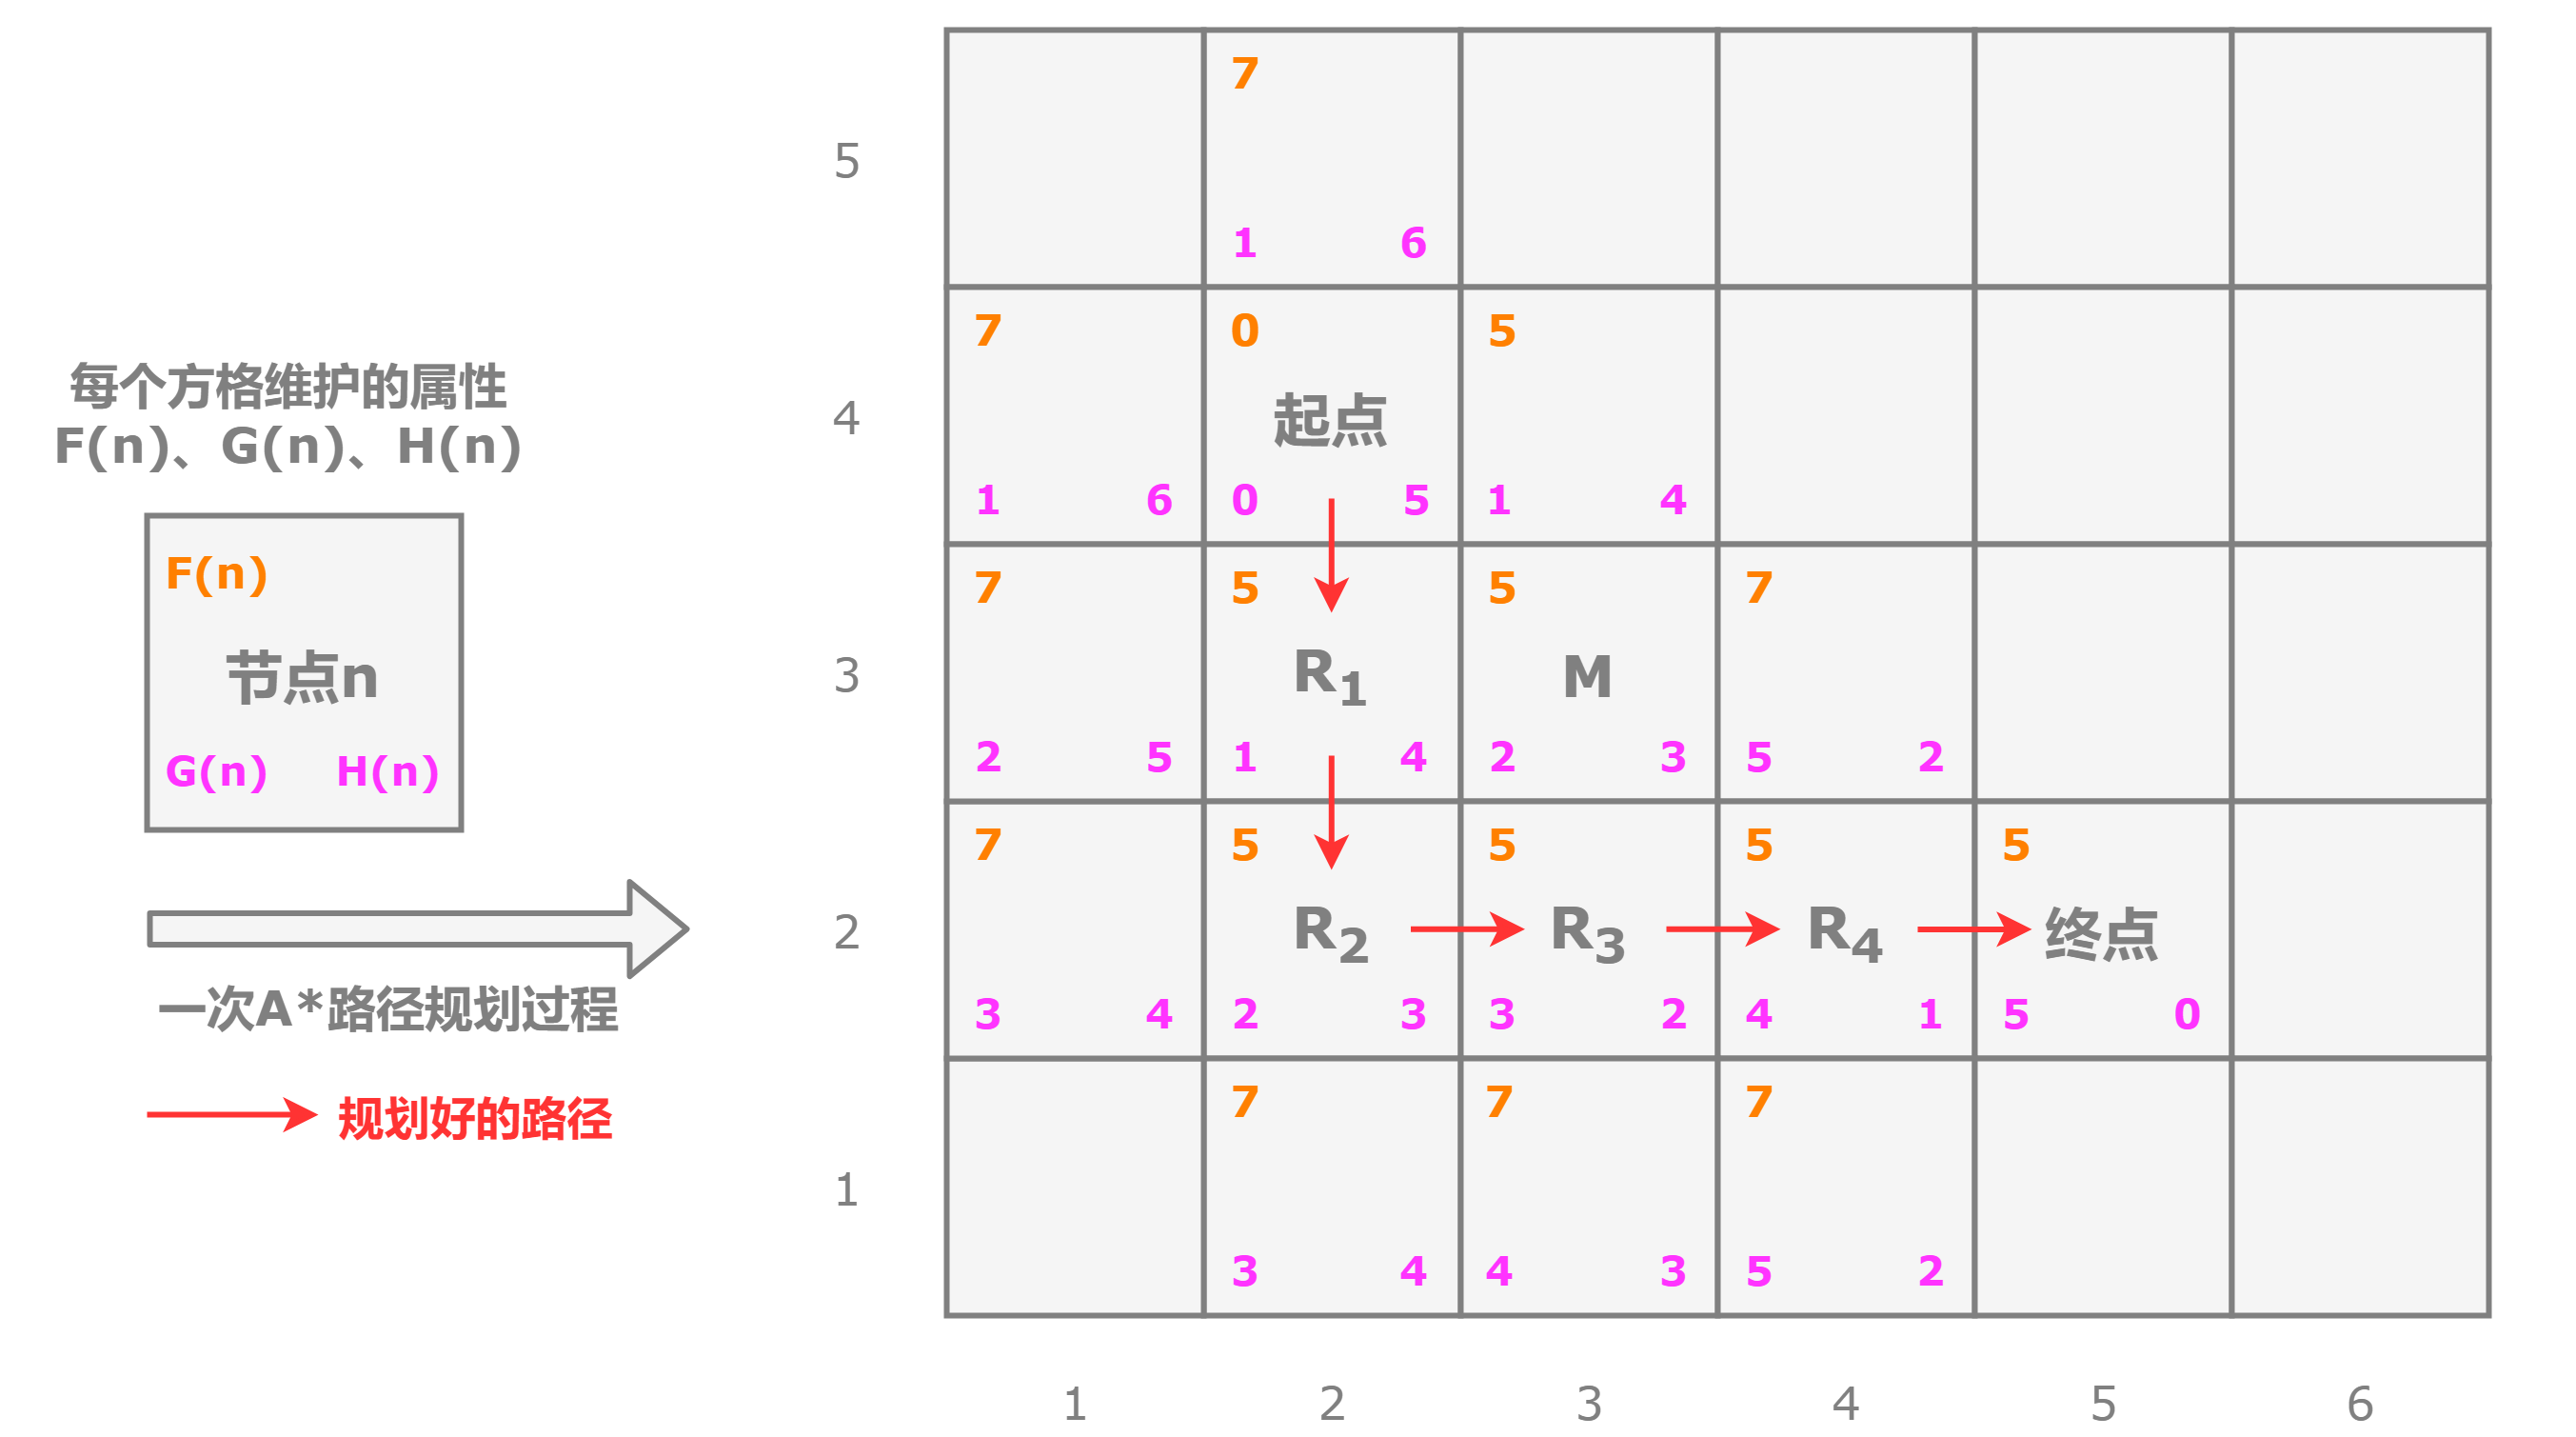
\includegraphics[width=0.8\textwidth]{undergraduate-thesis/images/Astar_Fn.png}
  \caption{A*算法示例}
  \label{AstarFn} % label 用来在文中索引
\end{figure}

图\ref{AstarFn}是A*算法运行过程的简单示意图。在该示意图中,假设一辆车需要从起点驶向终点,且该车辆只能朝上下左右四个方向驾驶,每个方格为正方形,边长为单位长度1,在计算启发函数H(n)时使用曼哈顿距离,并要求,如果计算出的总距离代价F相同,则优先朝下侧移动,再朝右侧移动,再朝上侧移动,最后朝左侧移动。

在上述场景中,结合图\ref{AstarFn},A*算法为起点与终点规划路径时的运行过程如下:

\begin{enumerate}
    \item 从起点到$R_1$点(第1轮):将起点位置加入Open表,然后从起点一圈圈向外寻找。首先找到的是起点的上下左右四个邻居方格,将它们加入Open表里,将起点加入Close表。分别计算这四个邻居方格的总距离代价F,得出起点下侧和右侧邻居的F同时最小,则按照假设,车辆向下侧移动,移至$R_1$点位,同时将$R_1$加入Close表中。
    \item 从$R_1$点到$R_2$点(第2轮):在$R_1$点位搜索邻居方格,发现起点作为$R_1$的上侧点位,实际上已经进入Close表中,因此,将$R_1$的左、右、下侧三个点加入Open表,作为邻居方格,并分别计算这三个邻居方格总距离代价F,得出$R_1$下侧和右侧邻居的F同时最小,按照假设,车辆向下侧移动至$R_2$点位,将同时将$R_2$加入Close表中。
    \item 从$R_2$点到$R_3$点(第3轮):在$R_2$点位搜索邻居方格,将$R_2$点位的左、右、下侧三个方格作为邻居方格,计算得到移动的下一个位置是$R_3$,将车辆移至$R_3$。
    \item 从$R_3$点到$R_4$点(第4轮):在$R_3$点位搜索邻居方格,将$R_3$的上、下、右侧三个方格作为邻居方格加入Open表中计算代价F。要注意的是,由于在第2轮中,邻居方格M已经被加入Open表,计算过一次总距离代价F,在本轮中,将对M重新计算总距离代价,所得代价较第2轮中计算的结果更高,因此不更新M在Open表中对应的F值。计算得到本轮移动的目的地为$R_4$。
    \item 从$R_4$点到终点(第5轮):在$R_4$点搜索邻居方格,将$R_4$的上、下、右侧三个邻居列入本轮的总距离代价计算过程中,结果是移至终点的F最小,因此将终点加入Close表,车辆的当前位置移动为终点,则路径规划成功,算法运行结束。
\end{enumerate}

在此例中,A*算法寻得的路径为:起点 -> $R_1$ -> $R_2$ -> $R_3$ -> $R_4$ -> 终点。

\subsection{传统A*算法与实时路况结合的必要性}

在章\ref{A*Reason}中,结合具体例子可知,A*算法有以下特性:

特性1:基于栅格法分割地图。

特性2:只关注静态的地图和方格间的距离本身。

针对A*算法的特性1,本文中的出租车调度系统基于Geohash编码的矢量地图数据,其借助Geohash编码将地图分成了大小相同的多个小方格,并且为每个地图中的运行道路都事先计算好用于反映路段距离的成本(cost)属性,该属性以米为单位。同时,本系统采用的启发函数是曼哈顿距离,符合地图数据和A*算法的方格特性。

针对A*算法的特性2,在真实的行车过程中,司机选择行驶道路的考虑因素是多方面的。路径长度是一个重要的考虑因素,同时,路况信息是另一个重要的考虑因素。路况信息能实时反映区域内的交通拥堵情况,便于司机估算前往目的地的用时,从而为司机提供一个最快捷、最通畅的最佳行驶路线。A*算法能够在起点和终点间搜寻到一条路程最短的规划路线,因此,在此基础上,引入实时路况的影响因子,才能更加真实地模拟汽车运行轨迹。

本文将在章\ref{A*New}中给出一种结合实时路况的改进A*算法设计。

\section{结合实时路况的改进A*算法}
\label{A*New}

\begin{figure}[!ht]
  \centering
  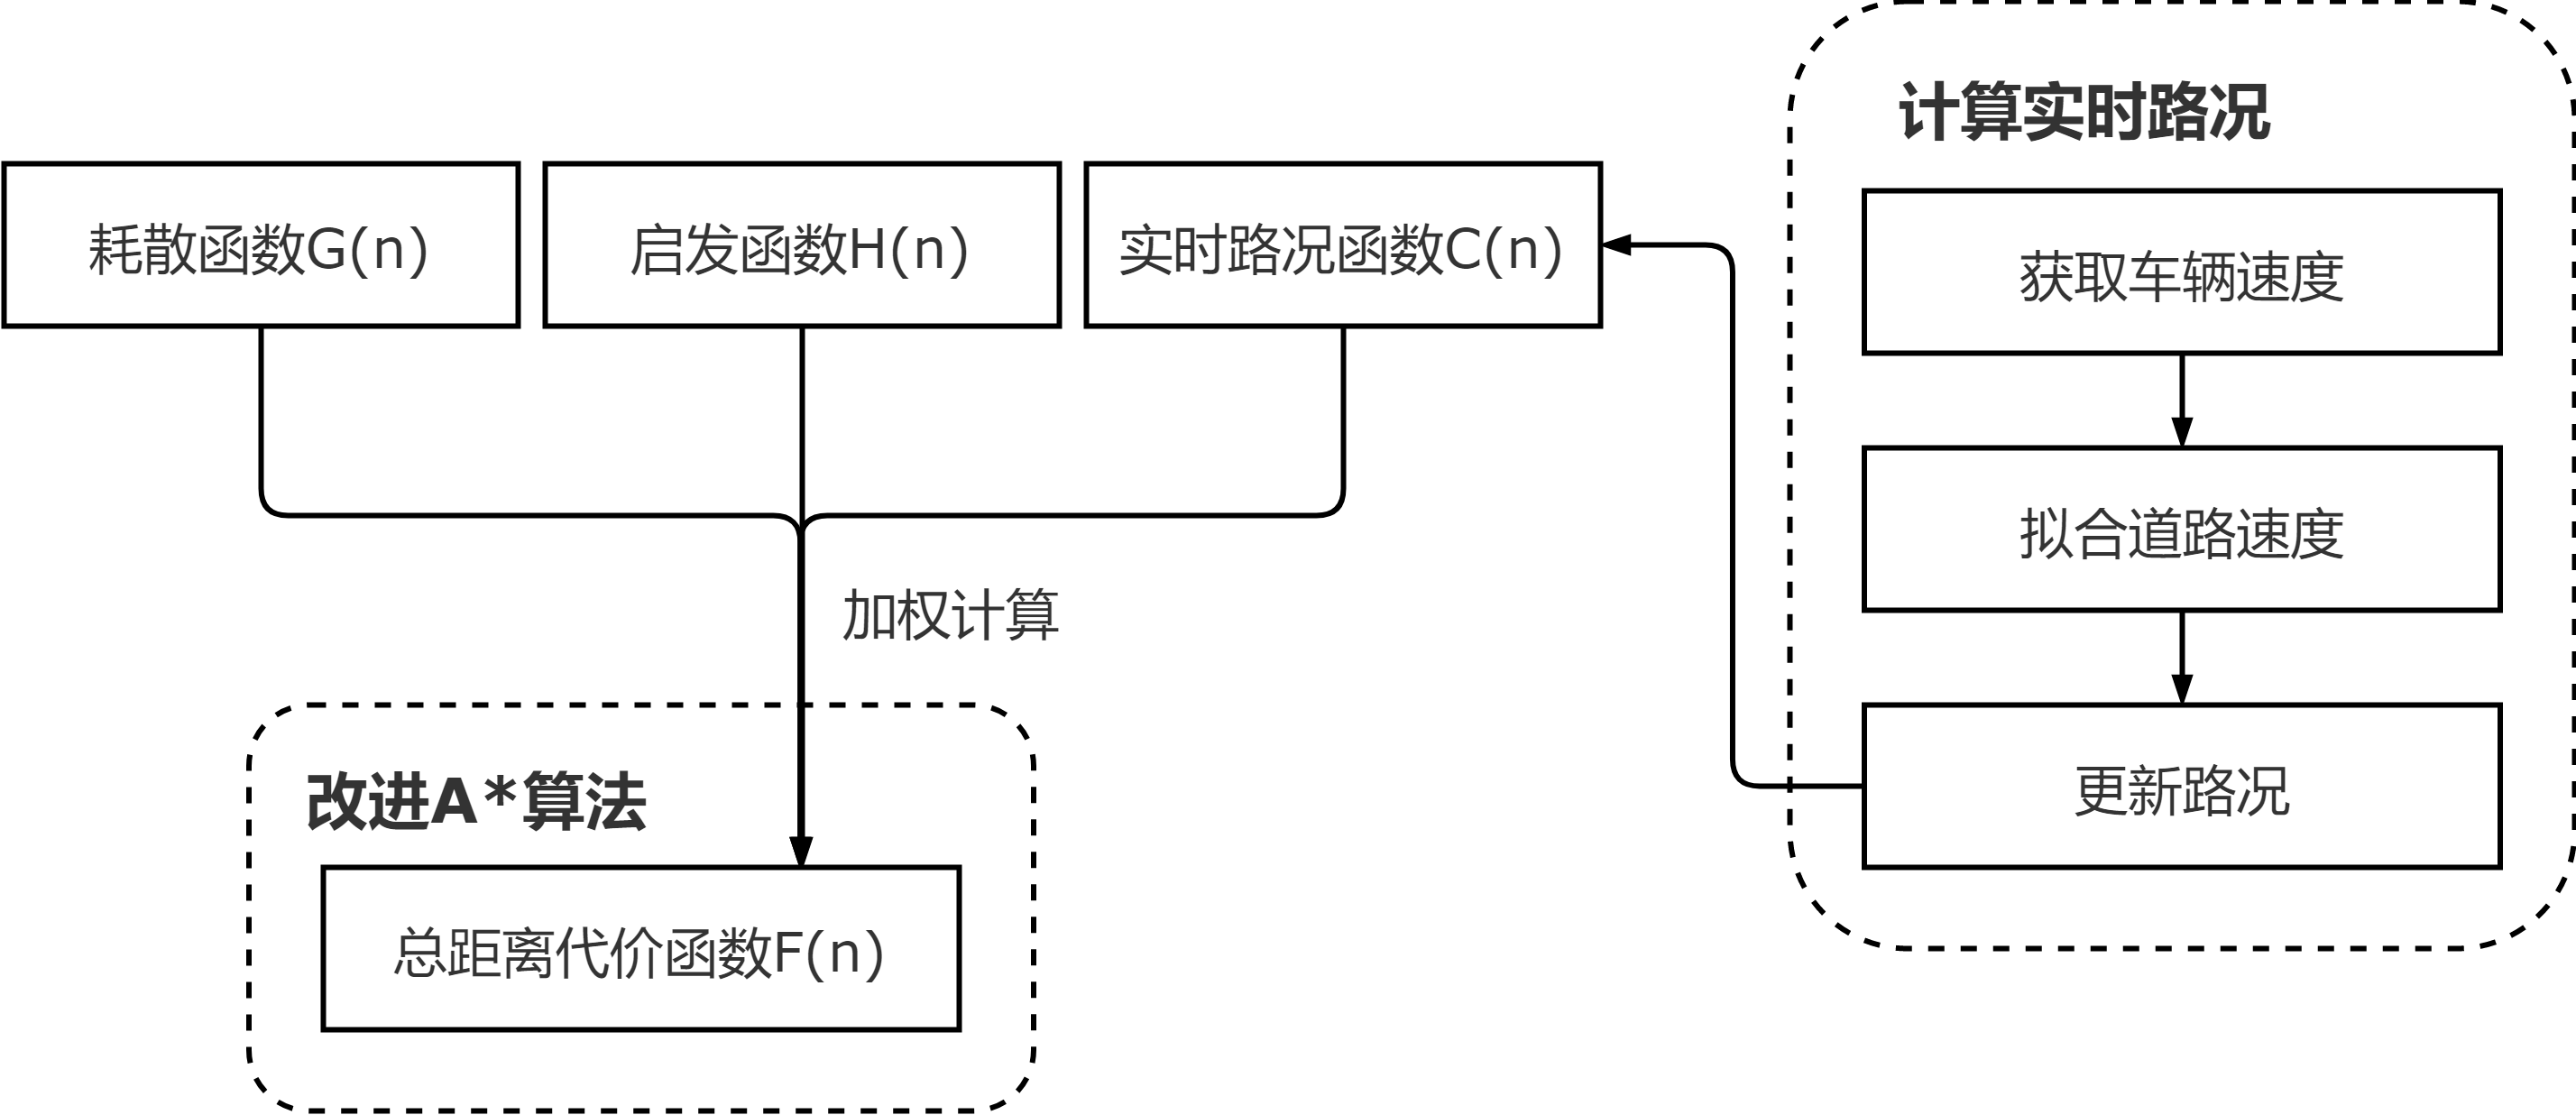
\includegraphics[width=0.7\textwidth]{undergraduate-thesis/images/Astar_new.png}
  \caption{结合实时路况的改进A*算法示意图}
  \label{newAstarIdea} % label 用来在文中索引
\end{figure}

本节设计了一种结合实时路况的改进A*算法,如图\ref{newAstarIdea}所示,本算法主要分为计算实时路况、改进A*算法两部分,在计算实时路况部分需要获取车辆速度、拟合道路速度、更新路况;在改进A*算法部分需要改动总距离代价函数F(n)的计算方式。

\subsection{符号与假设}

\begin{table}[ht]
  \linespread{1.5}
  \zihao{5}
  \centering
  \caption{符号表}\label{currentPathSymbols}
  \begin{tabular}{cc} 
  \toprule
    符号 & 含义 \\ 
  \hline
    $Round_i$ & 车辆运行的第i个轮次 \\
    $Vehicle_j$ & 第j辆车的名称 \\
    $Speed_j$ & 第j辆车的速度 \\
    $Distance_j$ & 第j辆车的行驶距离 \\
    $Time_j$ & 第j辆车的行驶时间 \\
    $V_{default}$ & 当前路段的限速,是道路的固定属性,永远不变 \\
    $V_{path,i}$ & 第i轮中,由n辆车拟合出的道路速度 \\ 
    $V_{History,i}$ & 第i轮中,道路的历史路况,是道路的属性 \\
    $V_{Current,i}$ & 第i轮中,道路的当前路况,是道路的属性 \\
    $V_{Fact,i}$ & 第i轮中,道路的实时路况,是道路的属性 \\
    F(n) & 节点n对应的总距离代价 \\
    G(n) & 节点n对应的耗散函数 \\
    H(n) & 节点n对应的启发函数 \\
    C(n) & 节点n对应的实时路况成本函数 \\
  \bottomrule
  \end{tabular}
\end{table}

章节\ref{A*New}中所用到的所有符号及其含义如表\ref{currentPathSymbols}中所示。其中,道路的历史路况$V_{History,i}$表示第$Round_{i-1}$轮计算出的实时路况,其在第$Round_{i-1}$轮中是实时路况,在第$Round_{i}$轮中成为历史路况;道路的当前路况$V_{History,i}$表示第$Round_{i}$轮中,由车辆拟合出的速度所代表的道路当前路况;道路的实时路况$V_{Fact,i}$表示第$Round_{i}$轮中,根据道路的历史路况和当前路况加权计算出的道路的实时路况,这是改进后的A*算法在进行路径规划时的主要依据之一。

%这图好像有点黑...
\begin{figure}[ht]
  \centering
  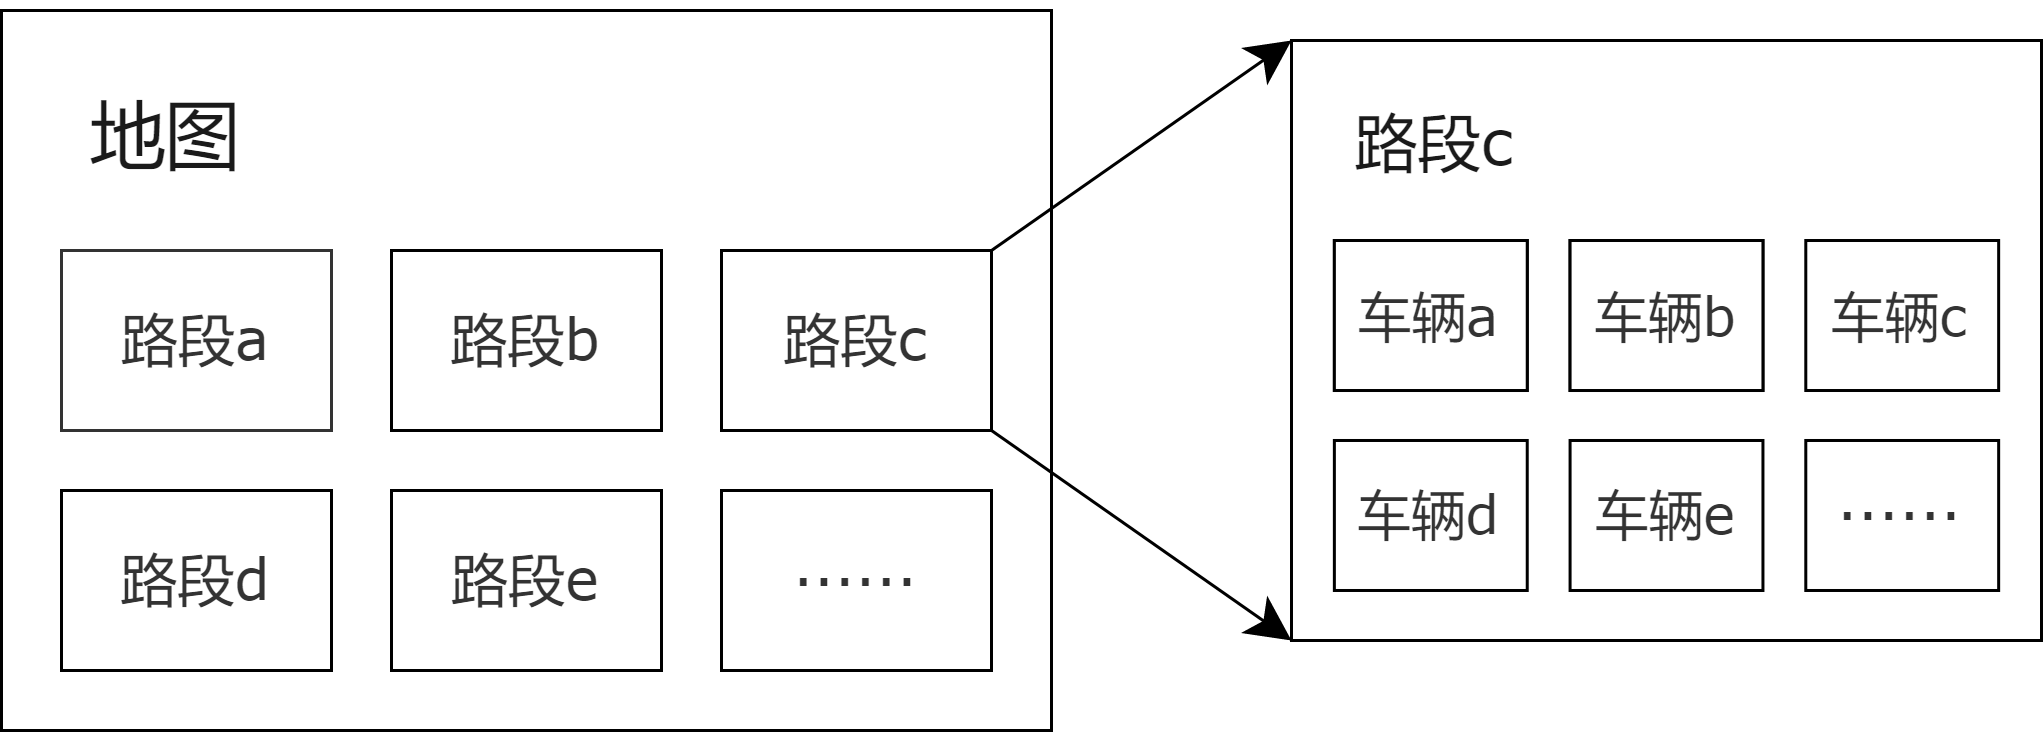
\includegraphics[width=0.7\textwidth]{undergraduate-thesis/images/MapPathVehicle.png}
  \caption{地图、路段、车辆的关系示意图}
  \label{mappathvehicle} % label 用来在文中索引
\end{figure}

图\ref{mappathvehicle}给出了本文系统中的三要素(地图、路段、车辆)关系。一份地图里会有$x(x>0)$个路段,在结合改进A*算法之后的出租车调度系统中,每个路段上会存在$y(y\ge 0)$辆车。

假设当前路段上存在运行中的车辆,假设一共有$n$辆车,这$n$辆车的起点为路段起点,这$n$辆车的终点为路段终点。这$n$辆车在当前路段运行一次,称为``车辆运行的第1个轮次”,在本轮运行完毕之后,这$n$辆车立刻回到原起点,等待下一轮运行,成为``车辆运行的第2个轮次”,这样循环往复,一共运行$m$轮。在这$m$轮的运行中,旧轮次的路况将成为影响新轮次路况计算的因素。

\subsection{实时路况的计算思路}
\label{subsection-calPathSituation}

每个城镇都包含成千上万条道路,随着城镇车辆的增加,道路拥堵现象已经成为普遍现象,尤其是在人群上下班的高峰期,道路拥堵的严重程度尤为突出。本节设计了一种计算实时路况的算法。

首先,是需要获取车辆速度。在获取车辆速度时,最常规的做法即利用车辆的运行距离$Distance$和运行时间$Time$计算车辆的速度。对$Round_k$中的第i辆车辆来说,其运行速度计算过程如公式\ref{calvspeed}。

\begin{equation}
    Speed_i = \frac{Distance_i}{Time_i} 
\label{calvspeed}
\end{equation}

其次,是需要拟合道路速度$V_{path}$。对道路速度的拟合计算,需要考虑路段中无车、有车两种情况。在道路无车时,如第一次初始化出每条道路时,没有车辆能影响当前道路的拟合速度,因此,道路的速度$V_{path}$等于其本身的固定属性限速$V_{default}$;在道路有车时,车辆速度将在不同程度上影响道路速度$V_{path}$,假设此时道路上一共有$n$辆车,第$i$辆车命名为$Vehicle_i$,其运行速度为$Speed_i$,则道路速度$V_{path}$的计算公式为取这些车辆的均值,如公式\ref{calpathSpeed}。
\begin{equation}
V_{path} =
  \left\{\begin{matrix}
  V_{default} & ,When\enspace there\enspace are\enspace no\enspace vehicles\enspace on\enspace the\enspace road. \\
  \frac{1}{n} {\sum_{i=1}^{n}Speed_i} & ,When\enspace there\enspace are\enspace vehicles\enspace on\enspace the\enspace road.
\end{matrix}\right.
\label{calpathSpeed}
\end{equation}

最后,需要按照前两步计算的内容,更新路况。其中,需以道路速度为量化数据代表路况。此时已通过$n$辆车的速度,综合起来计算得出了道路速度$V_{path}$。每个路段维护表\ref{currentPathSymbols}中的$V_{History}$、$V_{Current}$、$V_{Fact}$三个属性字段。在当前路段中,每轮有$n$辆车在道路上运行,一共运行$m$轮。

\begin{figure}[ht]
  \centering
  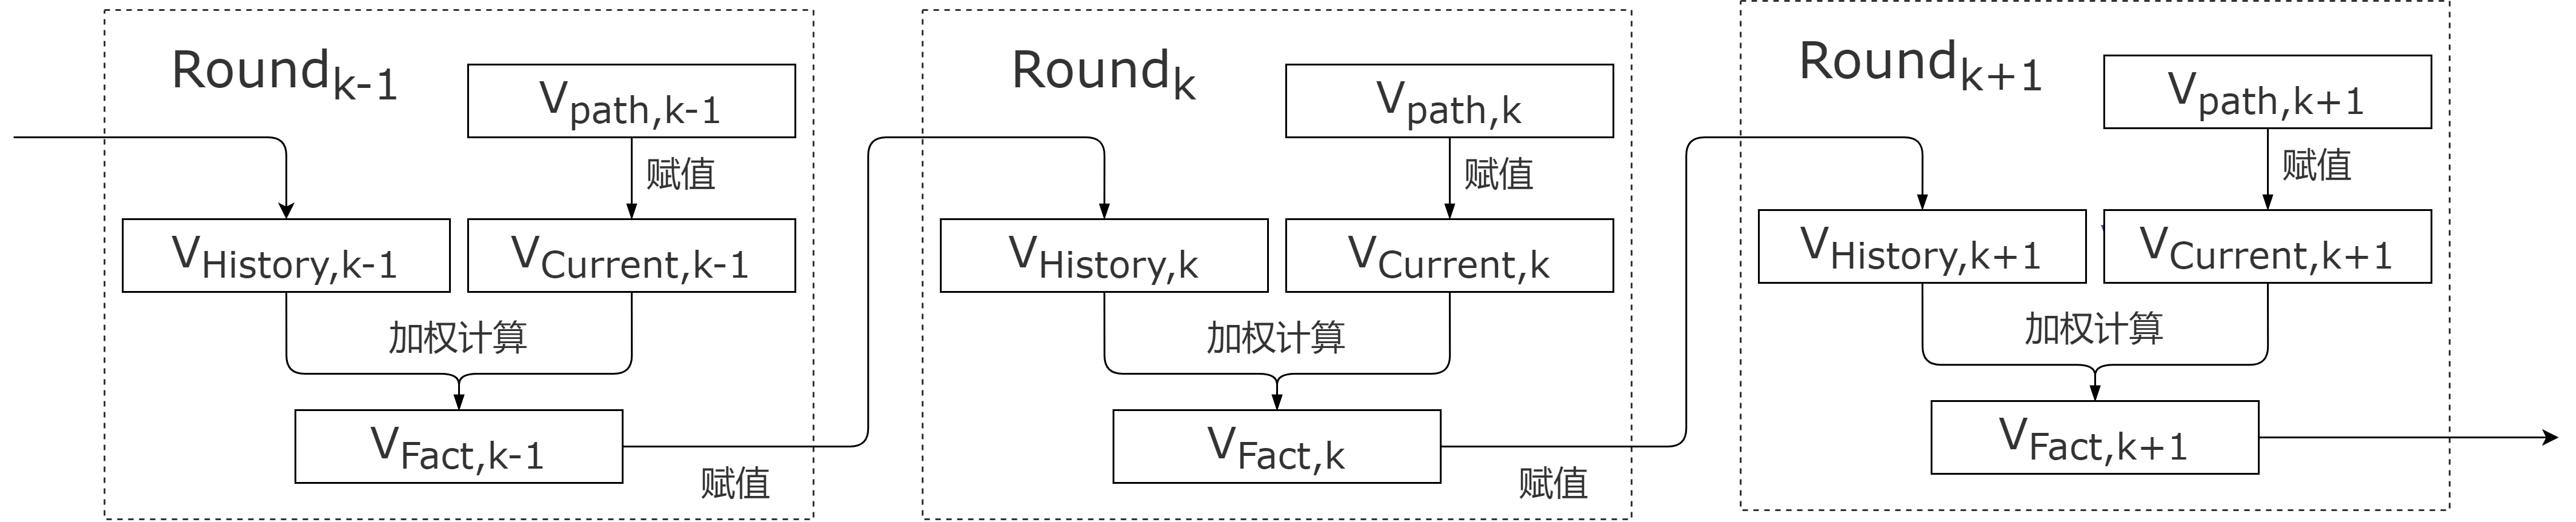
\includegraphics[width=1\textwidth]{undergraduate-thesis/images/calFactPathSituation.png}
  \caption{实时路况的迭代过程}
  \label{calFactPathSituation_pic} % label 用来在文中索引
\end{figure}

路况的计算是一个不断迭代的过程。如图\ref{calFactPathSituation_pic},设目前系统运行到了第$k$轮,则上一轮是第$k-1$轮,下一轮是第$k+1$轮。在上一轮中,路段的速度计算为$V_{Fact,k-1}$,本轮中路段的速度计算为$V_{path,k}$。则$V_{History,k}$、$V_{Current,k}$属性字段与路段速度的关系如公式\ref{calpathSituation}。该道路上一轮的通行速度$V_{Fact,k}$可以作为当前轮次的历史路况$V_{History,k}$。
\begin{equation}
    \left\{
    \begin{matrix}
    V_{History,k}=V_{Fact,{k-1}}
    \\
    V_{Current,k}=V_{path,k}
    \end{matrix}
    \right.
\label{calpathSituation}
\end{equation}

用公式\ref{calfact}计算第$k$轮的实时路况。其中,$\alpha$代表计算实时路况时的影响因子。$\alpha$越大,说明历史路况的权重越大,其对实时路况的影响效果越大,当前路况对实时路况的影响效果越小;$\alpha$越小,说明历史路况的权重越小,其对实时路况的影响效果越小,当前路况对实时路况的影响效果越大。
\begin{equation}
    V_{Fact,k}=\alpha V_{History,k}+(1-\alpha) V_{Current,k}
\label{calfact}
\end{equation}

在计算实时路况时,最关键的一步是通过公式\ref{calfact}对历史路况和当前路况进行加权计算。以$Round_k$轮为例,历史路况能在一定程度上反映上一轮结束时的路况;当前路况能在一定程度上反映本轮运行的路况。如果本轮结束时的实时路况$V_{Fact,k}$只参考上一轮结束时的路况$V_{Fact,k-1}$,则道路路况永远不会得到更新;如果本轮结束时的实时路况$V_{Fact,k}$只参考本轮运行的路况,则道路路况永远只受本轮车辆运行情况的约束,则一旦本轮车辆突然运行速度极慢,意味着当前道路中发生堵塞,将极大程度上影响路段路况$V_{Fact,k}$,使其立刻变低,这种情况下,道路会产生剧烈的震荡,它会导致其他车辆意识到该路段的堵塞情况,立刻远离该路段,但这种情况实际上是不现实的,现实生活中,尽管当前道路在一定时段内发生堵塞,依旧还会有车辆前往该路段通行。因此,将历史路况和当前路况进行加权计算得出实时路况是必要且符合现实情况的。

在用$\alpha$控制历史路况和当前路况对实时路况的影响效果时,$\alpha$的大小会影响历史路况和当前路况的权重,$\alpha$值的选取同样应该谨慎考虑上文所提及的道路震荡问题。当$\alpha=1$时,$V_{Fact,k}=V_{History,k}$,实时路况只取决于历史路况;当$\alpha=0$时,$V_{Fact,k}=V_{Current,k}$,实时路况只取决于当前路况;当$0<\alpha<1$时,$V_{Fact,k}$的影响因素将包含历史路况和当前路况。

选取影响因子$\alpha$的值时,还有以下可能性需要考虑:

1. $\alpha$较小:实时路况受历史路况影响较大。此时,当前路况的上传对实时路况的更新起不到太大的效果,实时路况将依然会趋于初始路况,不易改变,实时路况的更新效果将比较不理想。

2. $\alpha$较大:实时路况受当前路况影响较大。一旦当前路况计算出错,比如 --- 在通过路口、立交桥等地时,在未对此地区进行标注的情况下,可能会存在车辆移动距离为负数、通过当前路段时间过长等诸多问题。此时,实时路况很容易被这些问题影响,从而变得不可靠,从而影响实时路况更新效果的准确性。

在参考张禹\cite{张禹基于车辆轨迹的动态路况挖掘}和邱皓月\cite{孙卫真2019低采样率浮动车的路况计算精度优化}的工作后,本文将影响因子$\alpha$的值设定为0.8,完成实时路况的计算。

\subsection{改进A*算法的工作原理}

A*算法是静态的全局路径规划算法,其核心在于总距离代价函数F的计算。因此,要为A*算法引入实时路况影响因子,就需要对总距离代价函数F进行修改,如公式\ref{cal-newAstar}。在该公式中,保持原有A*算法的耗散函数G(n)和启发函数H(n)的计算方式不变,为达到添加实时路况影响因素的目的,新增实时路况成本计算函数C(n),其用于根据路段的实时路况计算当前路段的拥堵状况,从而为该路段赋予相应的权重,动态影响A*算法的路径规划结果。
\begin{equation}
    F(n)=G(n)+H(n)+C(n)
\label{cal-newAstar}
\end{equation}

本文在章\ref{subsection-calPathSituation}中,提及使用路段的速度$V_{path,k}$借助一系列计算过程,得出路段的实时路况$V_{Fact,k}$,用路段的实时路况来量化代表路段的拥堵情况。则对C(n)的计算,就通过路段的实时路况$V_{Fact,k}$处理而得到结果。
\begin{equation}
    C(n)=(V_{default}-V_{Fact,k})*\beta
\label{cal-C(n)}
\end{equation}

公式\ref{cal-C(n)}是本文所依赖的C(n)的计算过程。$V_{default}$是路段的限速数值,其代表在该路段绝对通畅的情况下,其上行驶的车辆所能驾驶的最大速度。$V_{Fact,k}$是路段的实时路况,其代表在第$Round_k$轮中,该路段上行驶的车辆实际驾驶速度拟合的结果。$V_{default}$与$V_{Fact,k}$作差所得的结果,代表该路段的实时路况与完全通畅的路况的速度差$\Delta V$。

$\Delta V$越大,代表道路越拥堵,则此时在路段的驾驶过程是困难的,此时当前路段的实时路况成本会增大,对应的由A*算法计算出的总距离代价也会增大,从而在一定程度上减少第$Round_{k+1}$轮中车辆在此路段通行的可能性。

$\Delta V$越小,代表道路越通畅,则此时在路段的驾驶过程是容易的,此时当前路段的实时路况成本C(n)较小,对应的由A*算法计算出的总距离代价也会更接近G(n)+H(n)。这种情况下,由于路段通畅,所以路段上车辆的运行对A*算法计算出的总距离代价不会造成太大影响,从而在一定程度上增大第$Round_{k+1}$轮中车辆仍在此路段通行的可能性。

仍以章\ref{A*Reason}中的图\ref{AstarFn}对应的情景为例,以下给出结合实时路况的改进A*算法在此图中的路径规划过程和结果。

\begin{figure}[ht]
  \centering
  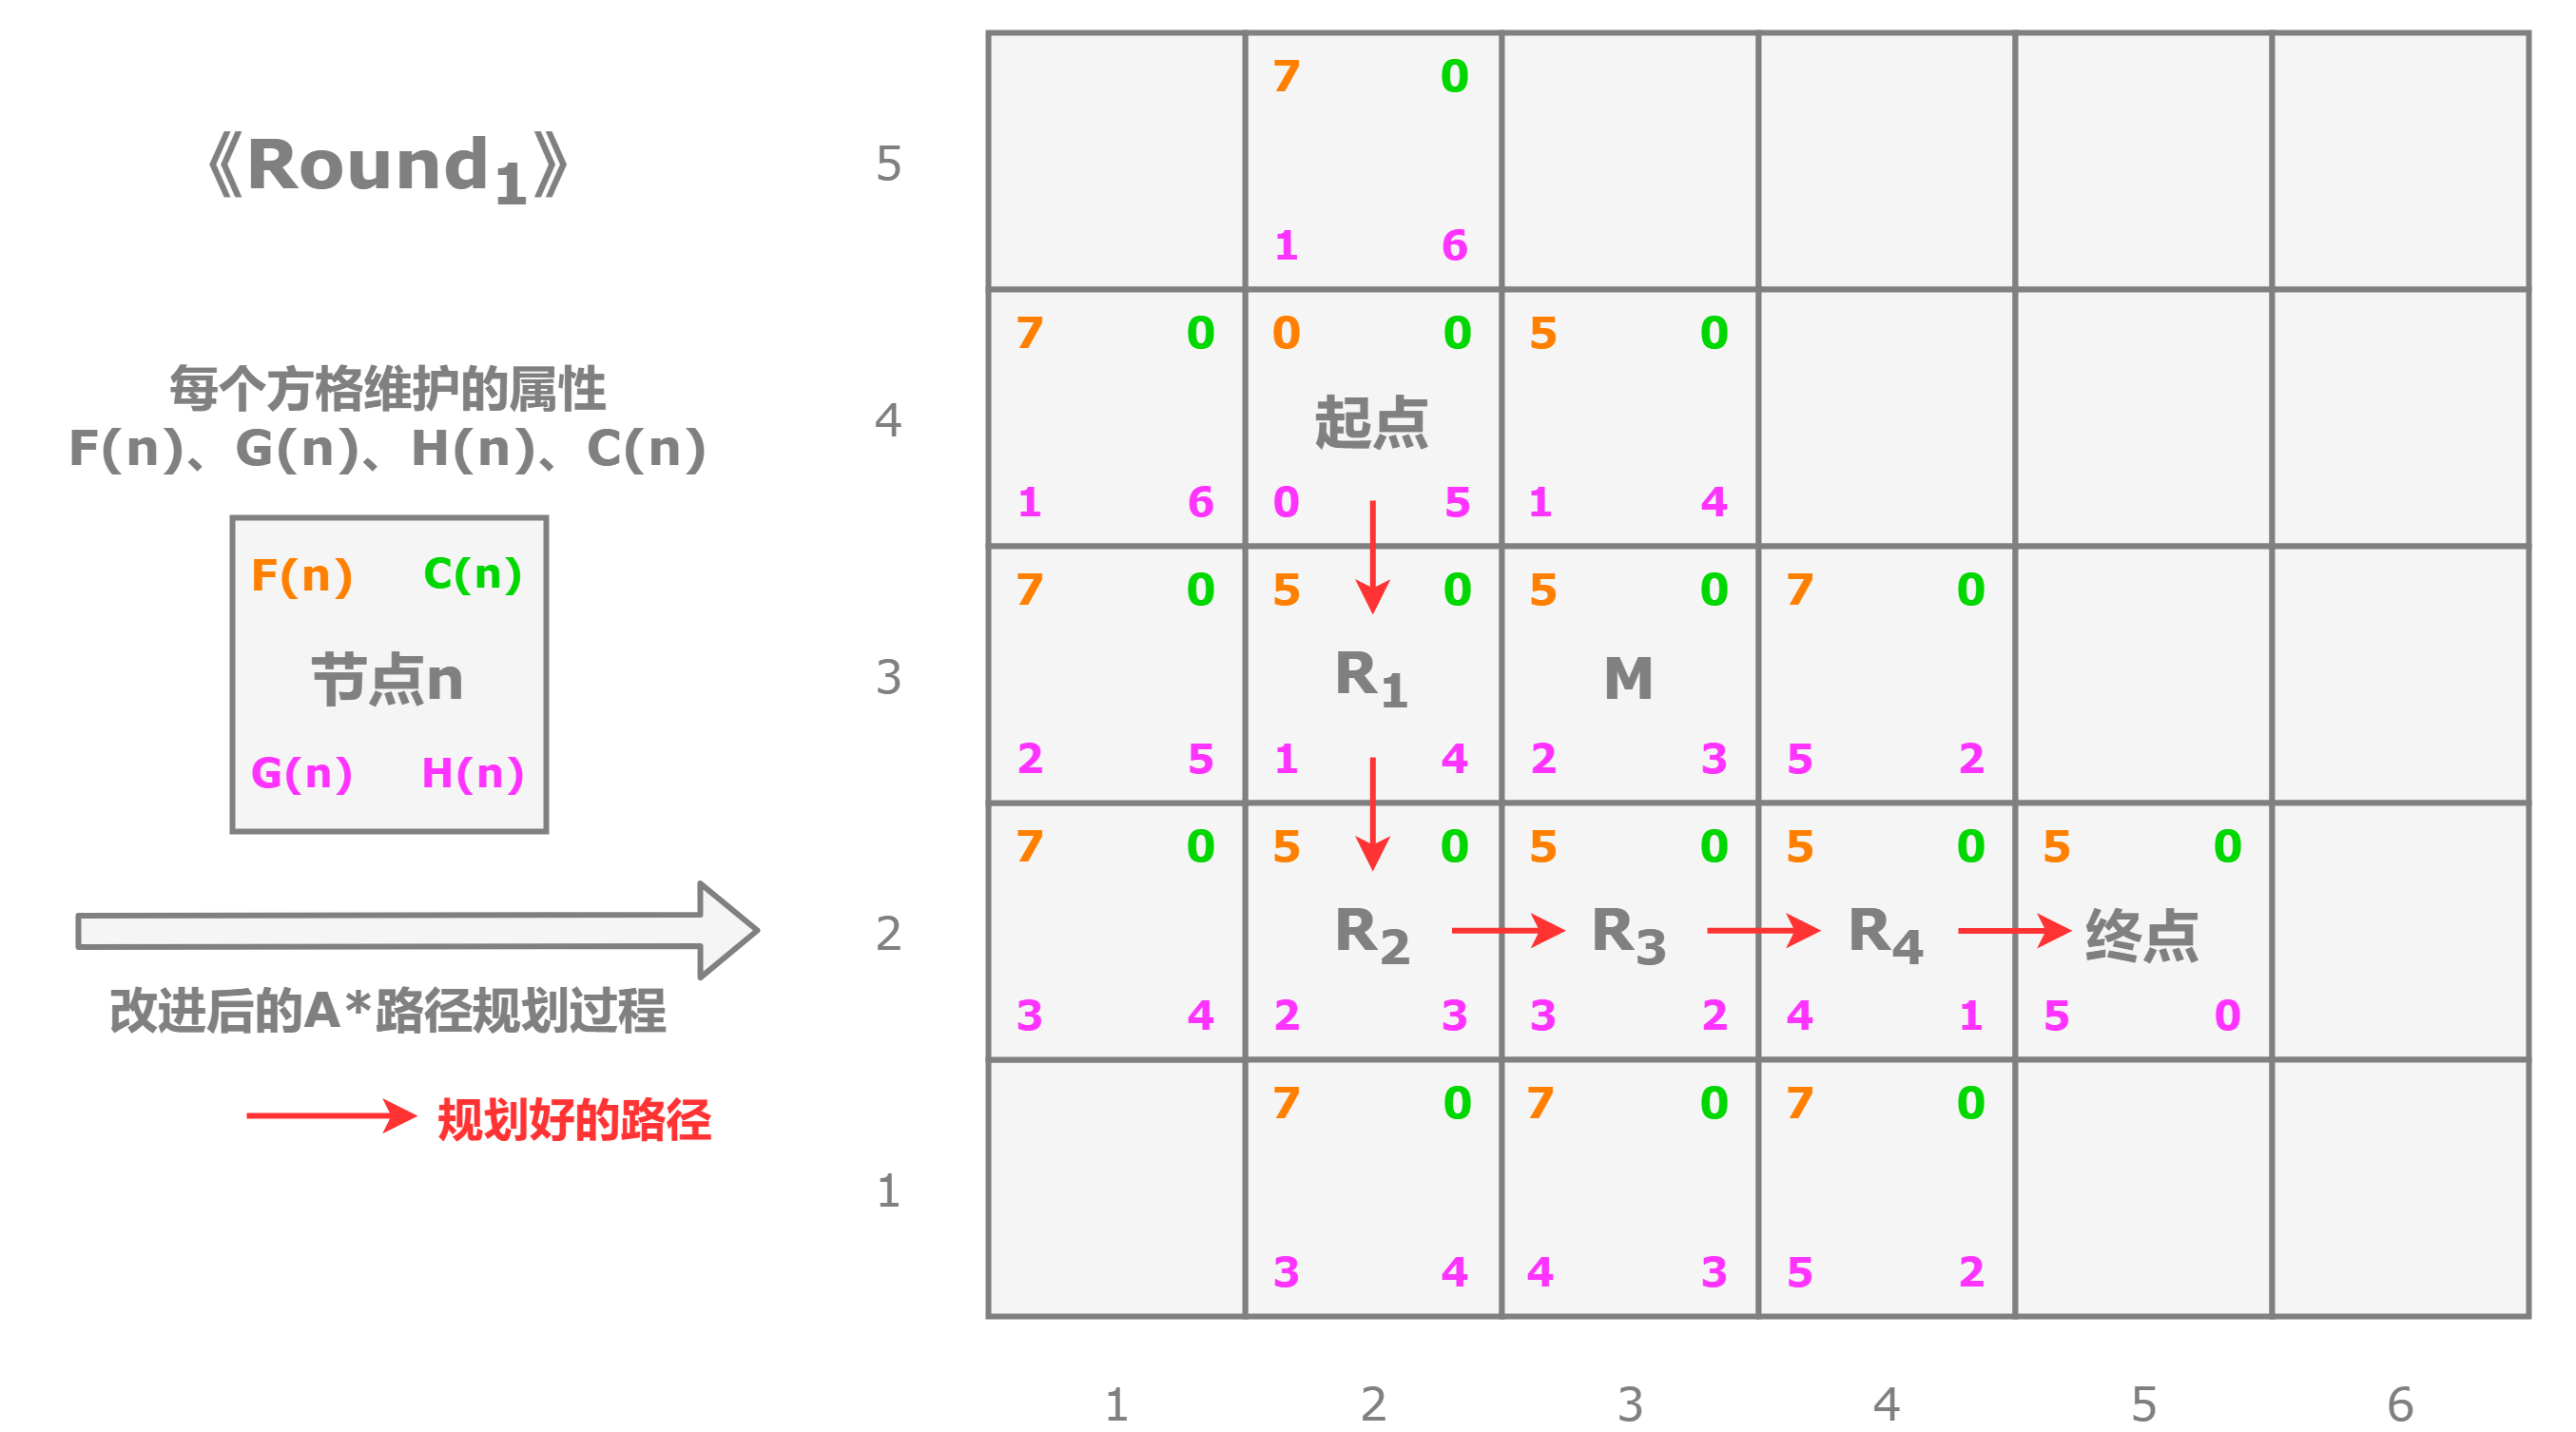
\includegraphics[width=0.75\textwidth]{undergraduate-thesis/images/Astar_newFnRound1.png}
  \caption{结合实时路况的改进A*算法($Round_1$)示例}
  \label{AstarnewFnR1} % label 用来在文中索引
\end{figure}

假设此系统一共运行2轮,在第1轮运行时,由于此前从未有车辆在该地图上行驶过,则第1轮运行时,所有道路的$V_{path}$都与道路的限速$V_{default}$一致,即此时相当于没有上一轮的实时路况,结合实时路况的改进A*算法规划出的路径与A*算法规划出的路径是一致的,如图\ref{AstarnewFnR1}中所示结果,规划出的路径为:起点 -> $R_1$ -> $R_2$ -> $R_3$ -> $R_4$ -> 终点。

由于第1轮车辆完成了一轮运行,此时已存储了$Round_1$的路况信息,则该路况信息将对$Round_2$中的路径规划产生影响。

\begin{figure}[ht]
  \centering
  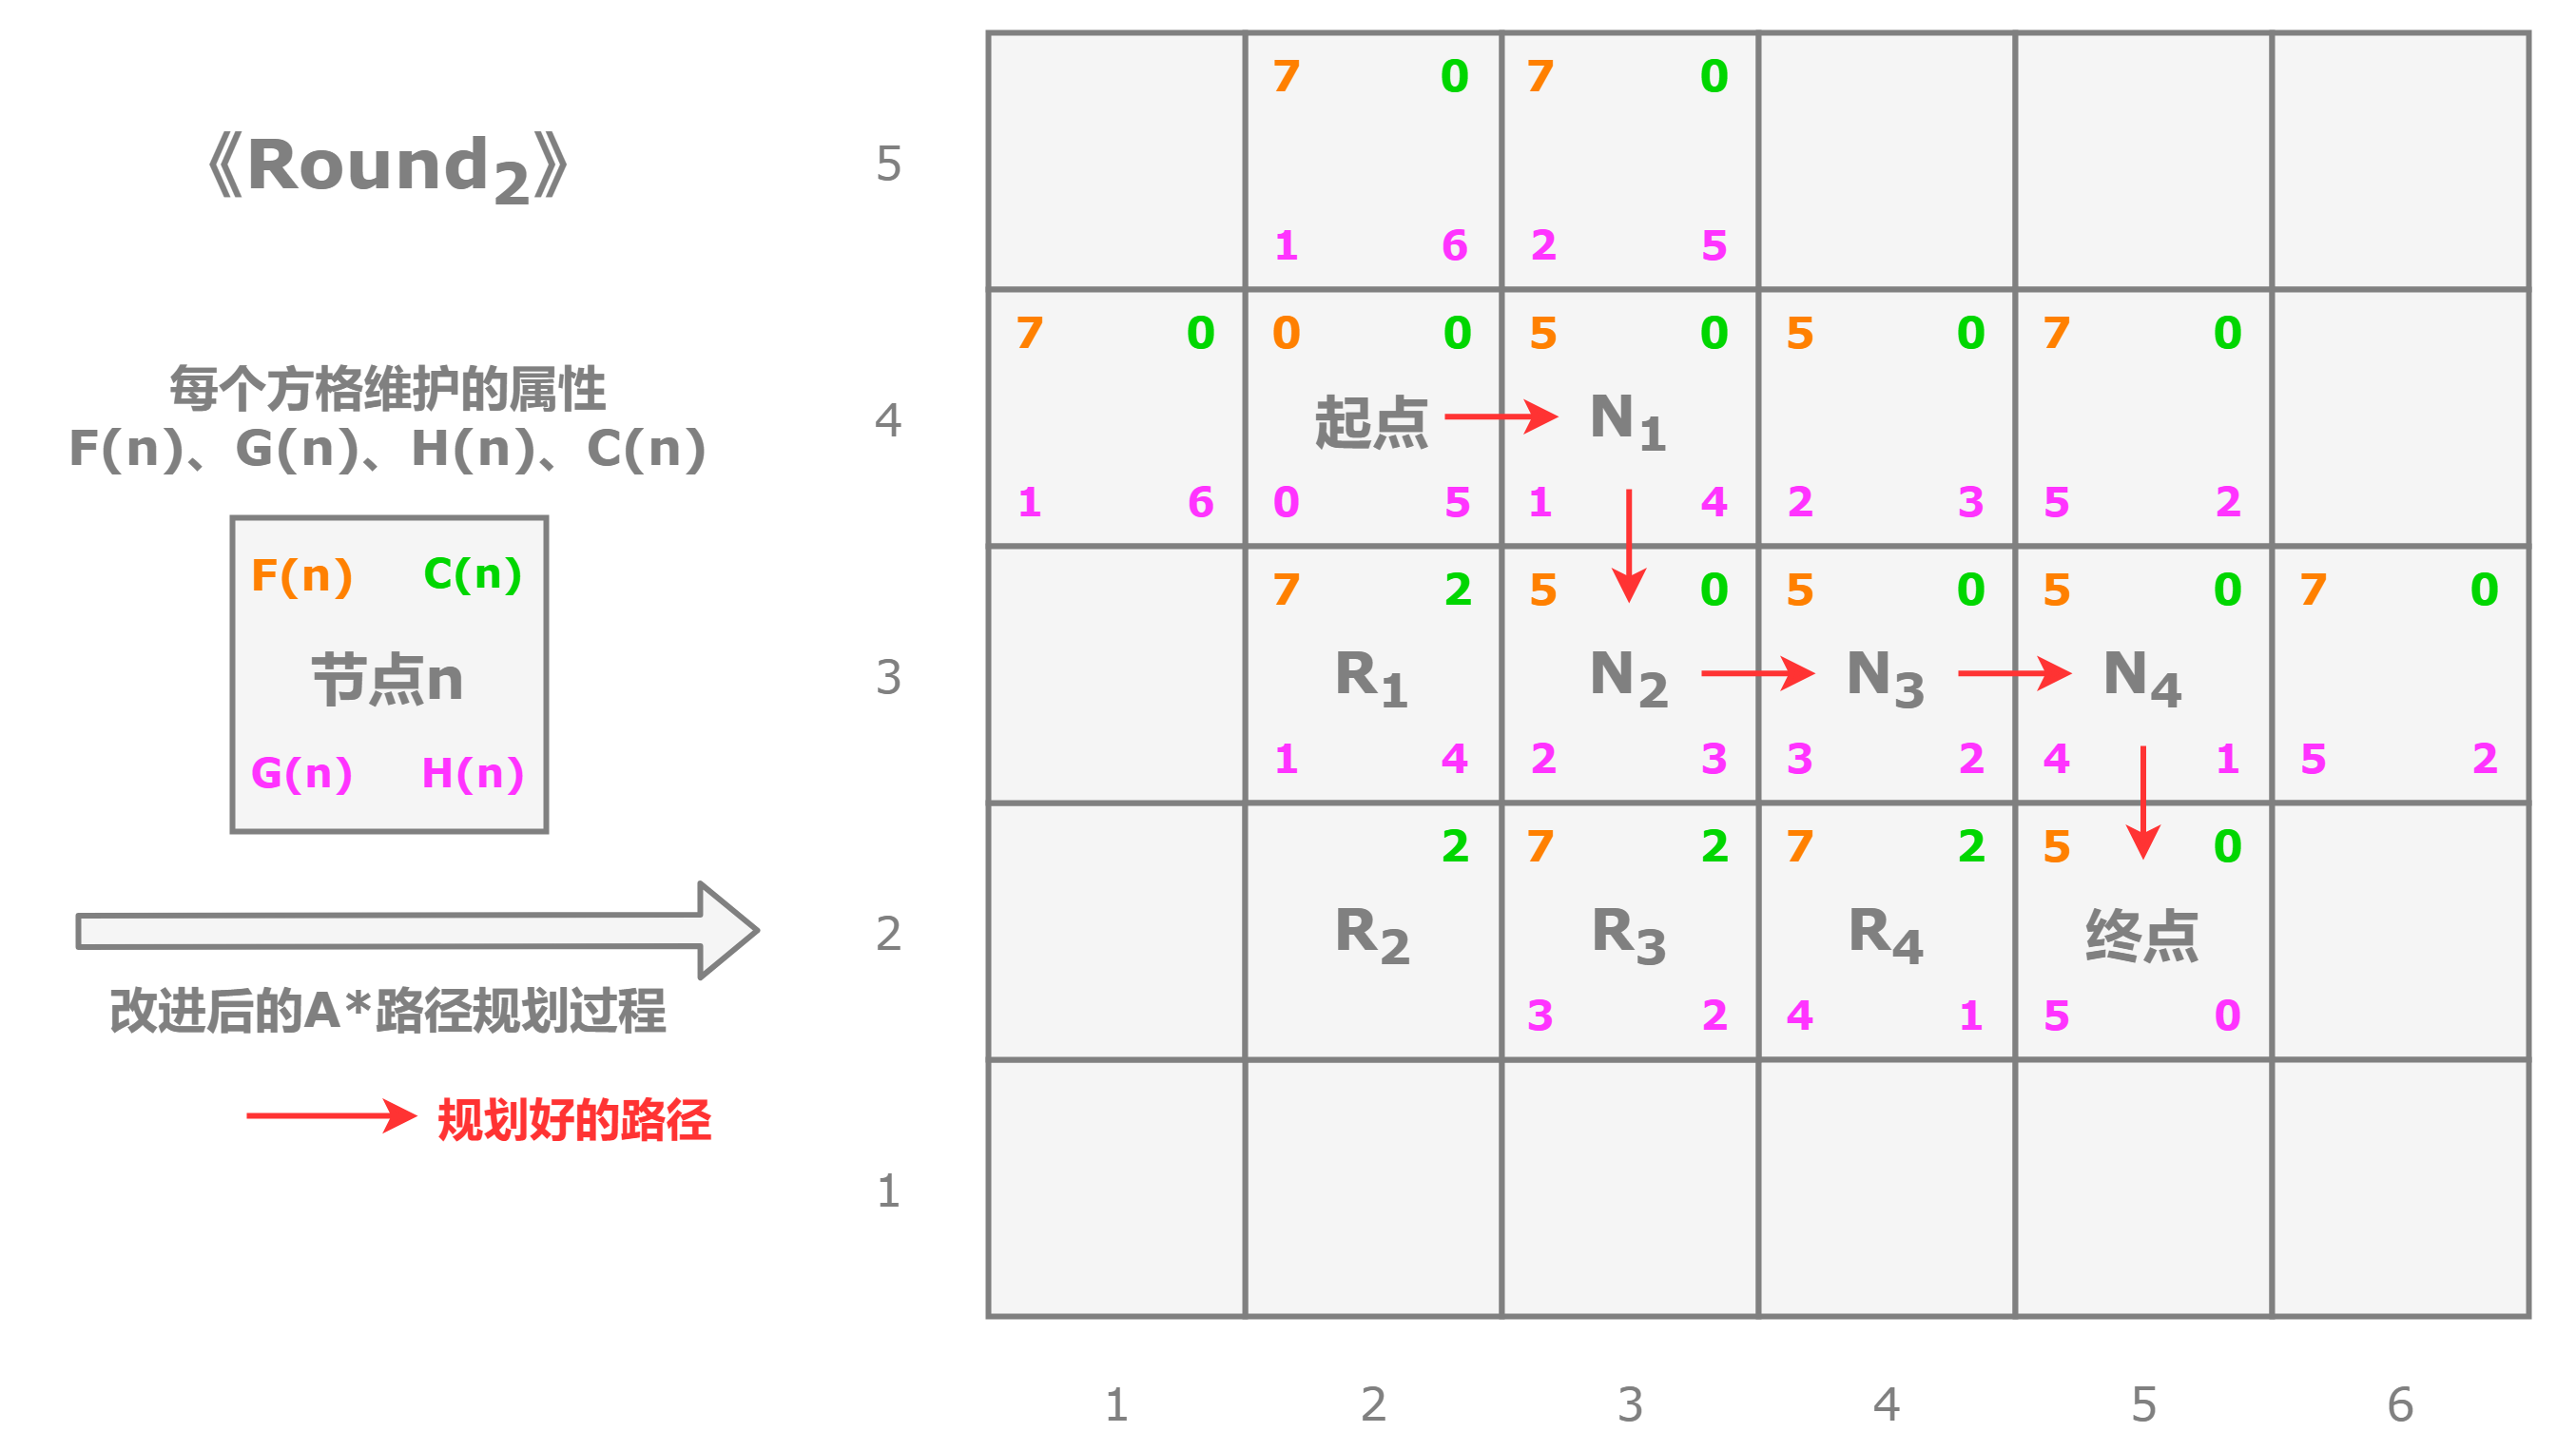
\includegraphics[width=0.75\textwidth]{undergraduate-thesis/images/Astar_newFnRound2.png}
  \caption{结合实时路况的改进A*算法($Round_2$)示例}
  \label{AstarnewFnR2} % label 用来在文中索引
\end{figure}

$Round_1$中规划好的路径,视作已经有车运行过了,为已走过的道路($R_1$、$R_2$、$R_3$、$R_4$)赋C(n)=2,则在$Round_2$中车辆再次从起点驶向终点时,路径规划的过程如图\ref{AstarnewFnR2}所示,结合实时路况的改进A*算法在$Round_2$中的运行过程为:

\begin{enumerate}
    \item 从起点到$N_1$点(第1轮):将起点位置加入Open表,然后从起点向外寻找。首先找到的是起点的上下左右四个邻居方格,将它们加入Open表里,将起点加入Close表。分别计算这四个邻居方格的总距离代价F,得出起点右侧邻居的F最小,则车辆向右侧移动,移至$N_1$点位,同时将$N_1$加入Close表中。
    \item 从$N_1$点到$N_2$点(第2轮):在$N_1$点位搜索邻居方格,发现起点作为$N_1$的左侧点位,实际上已经进入Close表中,因此,将$N_1$的上、右、下侧三个点加入Open表,作为邻居方格,并分别计算这三个邻居方格总距离代价F,得出$N_1$下侧和右侧邻居的F同时最小,按照假设,车辆向下侧移动至$N_2$点位,将同时将$N_2$加入Close表中。
    \item 从$N_2$点到$N_3$点(第3轮):在$N_2$点位搜索邻居方格。$N_2$点位的左、右、下侧三个方格作为邻居方格,但$R_1$格实际上已经在第1轮中计算过F,因此,此时重新计算$R_1$的总距离代价,所得代价较第1轮计算更高,因此不更新$R_1$在Open表中对应的F值。计算得到移动的下一个位置是$N_3$,将车辆移至$N_3$。
    \item 从$N_3$点到$N_4$点(第4轮):在$N_3$点位搜索邻居方格,将$N_3$的上、下、右侧三个方格作为邻居方格加入Open表中计算代价F。得出$N_3$上侧和右侧邻居的F同时最小,按照假设,车辆向右侧移动至$N_4$点位,将同时将$N_4$加入Close表中。
    \item 从$N_4$点到终点(第5轮):在$N_4$点搜索邻居方格,将$N_4$的上、下、右侧三个邻居列入本轮的总距离代价计算过程中,结果是移至终点的F最小,因此将终点加入Close表,车辆的当前位置移动为终点,则路径规划成功,算法运行结束。
\end{enumerate}

在此例中,经过$Round_1$与$Round_2$两轮运行后,A*算法在$Round_2$中寻得的路径为:起点 -> $N_1$ -> $N_2$ -> $N_3$ -> $N_4$ -> 终点。达到了路径规划基于实时路况而实时更新的结果,说明此算法是正确且可行的。

\section{结合实时路况的改进A*算法在调度系统中的实现}
\label{section_useNewAstarinTaxiSystem}
% 更新——————————————
Solidity语言是一种面向智能合约的、图灵完备的高级编程语言,它由以太坊提供,在以太坊虚拟机(EVM)上运行。Solidity是面向对象的语言,它具有静态的特性,支持继承、类库、用户自定义类型等特性。Solidity是目前较常应用于以太坊的语言。Remix-ide是一款基于浏览器的Solidity编译器,它可以在线使用。本文使用Solidity语言完成智能合约的开发,使用Remix-ide完成对智能合约的编译。

\begin{figure}[ht]
  \centering
  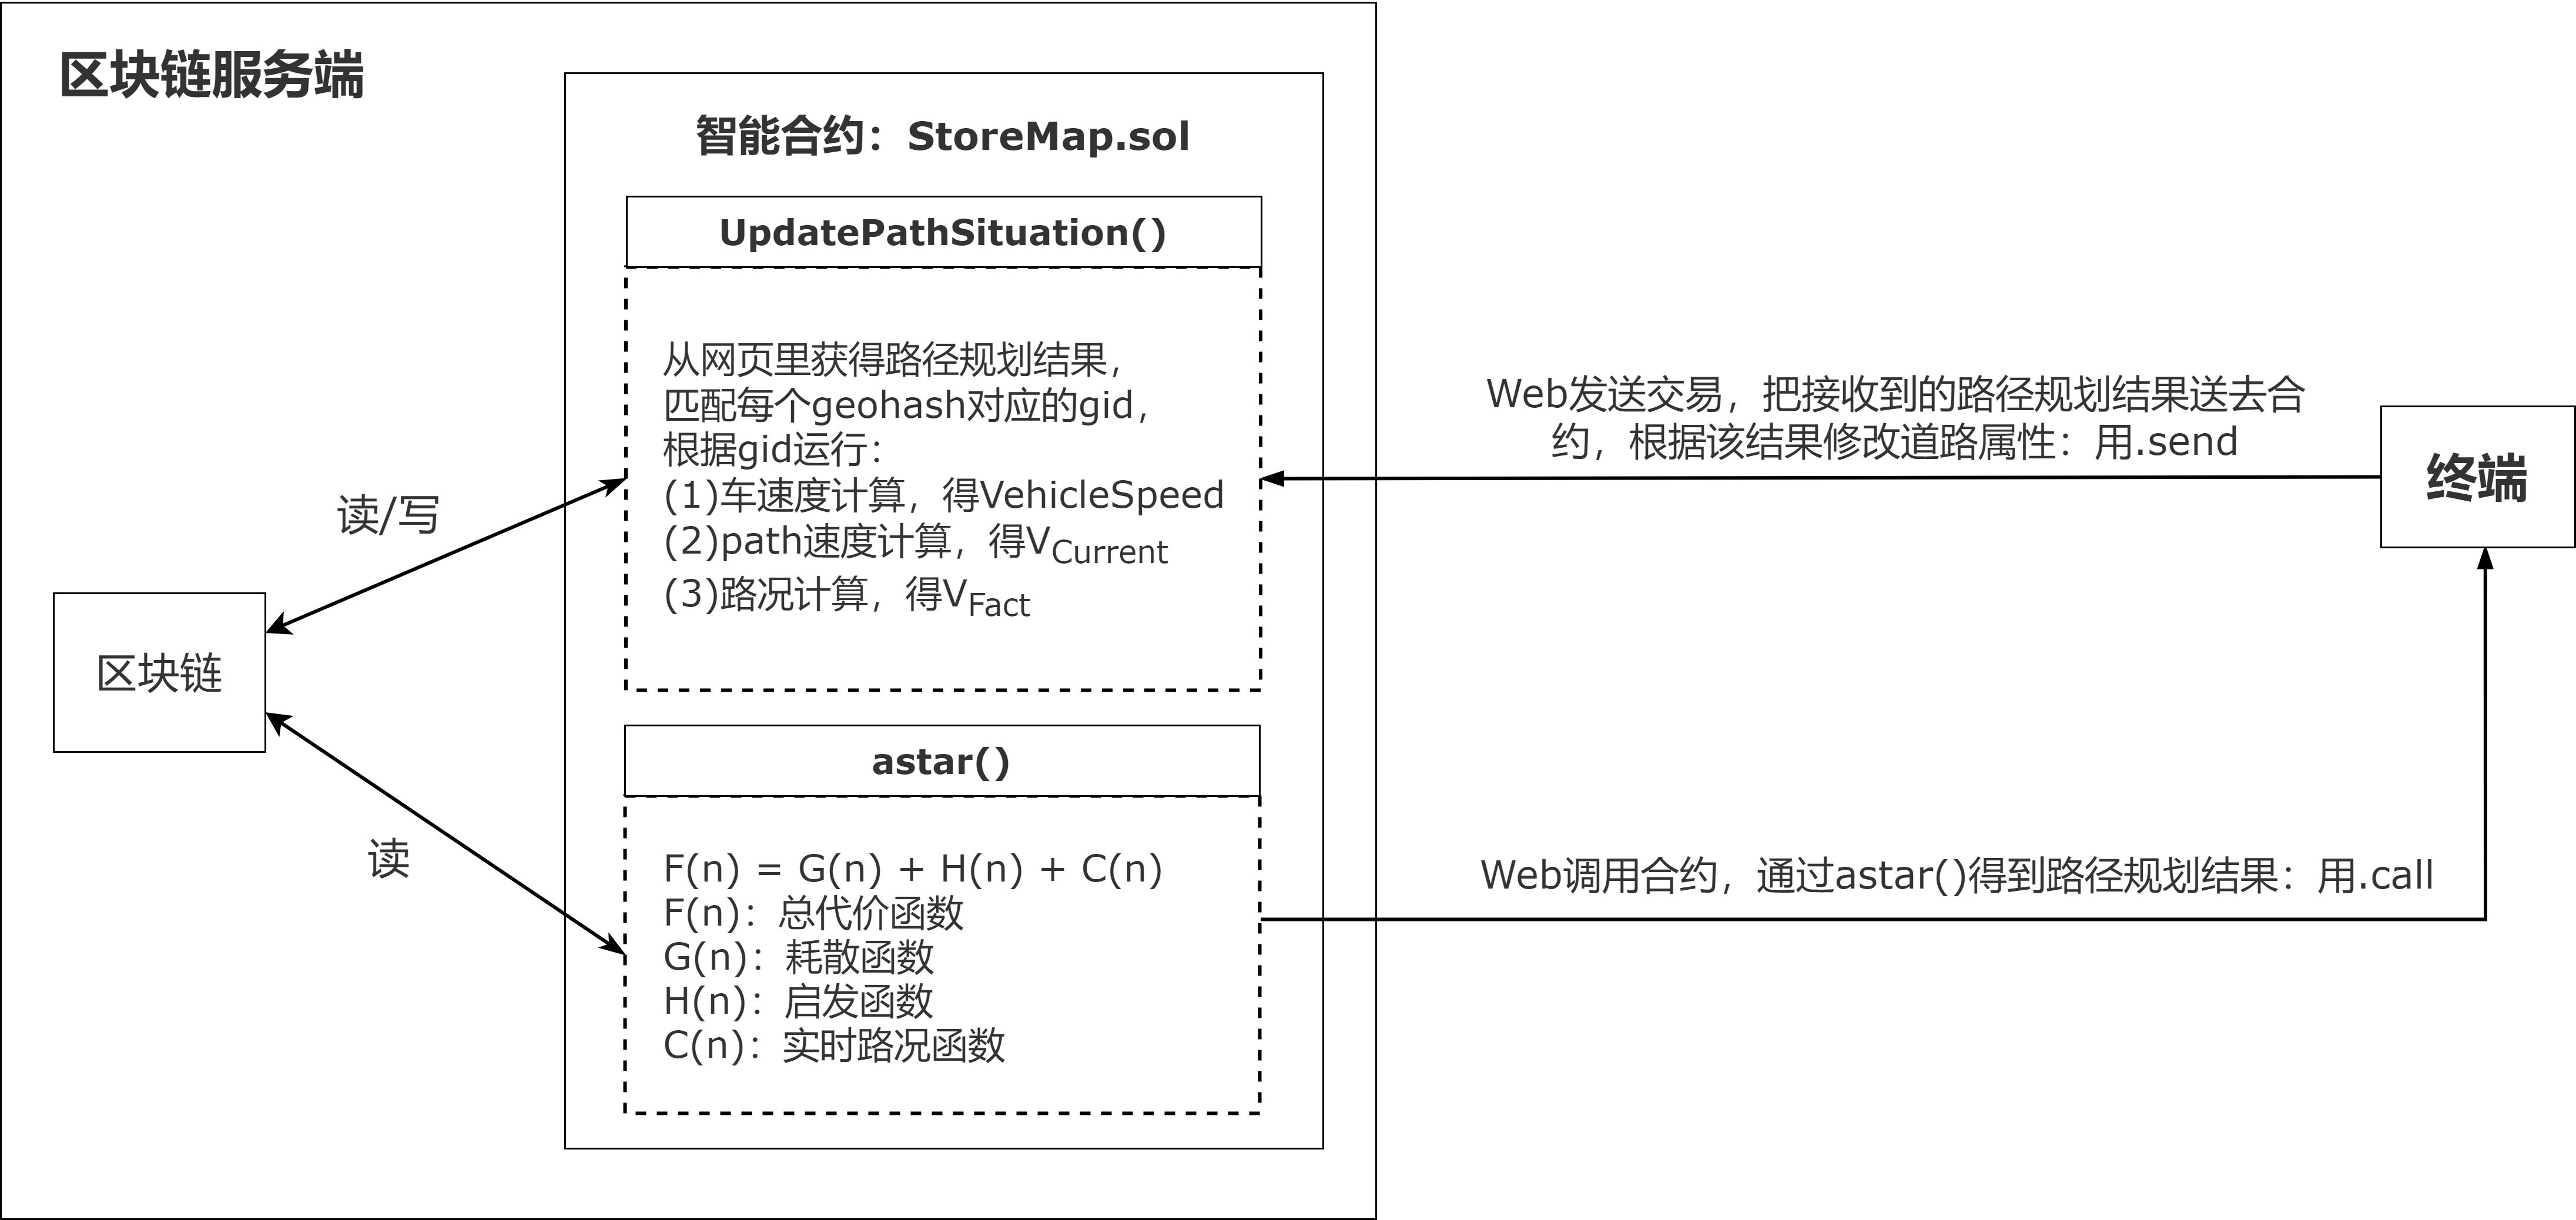
\includegraphics[width=0.8\textwidth]{undergraduate-thesis/images/AlgorithmInteractive.png}
  \caption{实现思路示意图}
  \label{algorithm-interactive} % label 用来在文中索引
\end{figure}

在已有的出租车调度系统中,主要的实现思路如图\ref{algorithm-interactive}。整个系统分为智能合约、区块链、网页端三大部分。智能合约部署在区块链上,由网页端通过调用智能合约内函数的方式与区块链交互。具体到本算法中,先打开树状区块链,在其上部署智能合约,并上传地图,最后打开python脚本用自动化工具selenium自动控制Web网页行为,运行系统。
% 设置三线表
\begin{table}[ht]
    \linespread{1.5}
    \zihao{5}
    \centering
    \caption{函数调用方法区别}
    \label{callandsend}
    \begin{tabular}{cc}
    \toprule
    .call & .send\\
    \hline
    不修改链上数据 & 修改链上数据 \\
    函数可以返回数据 & 函数不返回数据 \\
    函数立刻执行 & 函数花费一段时间执行完毕 \\
    免费 & 花费gas \\
    \bottomrule
    \end{tabular}
\end{table}
% 结束设置三线表

智能合约中,UpdatePathSituation()用于实时路况的计算和更新,它对链上存储的数据进行读和写操作;astar()用于运行改进的A*算法规划路径,它只需要对链上数据进行读取。因此这两个函数在调用时,参考表\ref{callandsend},前者用call调用,后者用send调用。

Web网页通过调用astar()来完成基于实时路况的路径规划,在获取到改进A*算法调度出的路径之后,将此路径规划结果打包为交易的方式,以输入参数的形式提交给UpdatePathSituation(),通过智能合约修改区块链上与实时路况相关的道路属性数据,实现实时路况的更新。在系统的下一轮运行时,Web网页再次调用astar(),就将根据区块链上新的道路属性数据计算道路的总距离成本,实现路径规划,从而进行动态路径规划过程。

在已有的出租车调度系统中一共需要部署3个合约,这三个合约分别被命名为StoreMap.sol、StoreTraffic.sol、Credit.sol。StoreMap.sol的功能是完成地图的存储、前端的匹配、用A*算法实现路径规划;StoreTraffic.sol的功能是进行车辆与乘客的系列操作(包括初始化车辆与乘客的位置、设置车辆与乘客的起点和终点、修改乘客与车辆的状态等)、乘客确认上车、乘客支付路费、存储和获取A*算法计算所得的路径;Credit.sol的功能是完成车辆信誉值的计算。

\begin{figure}[ht]
  \centering
  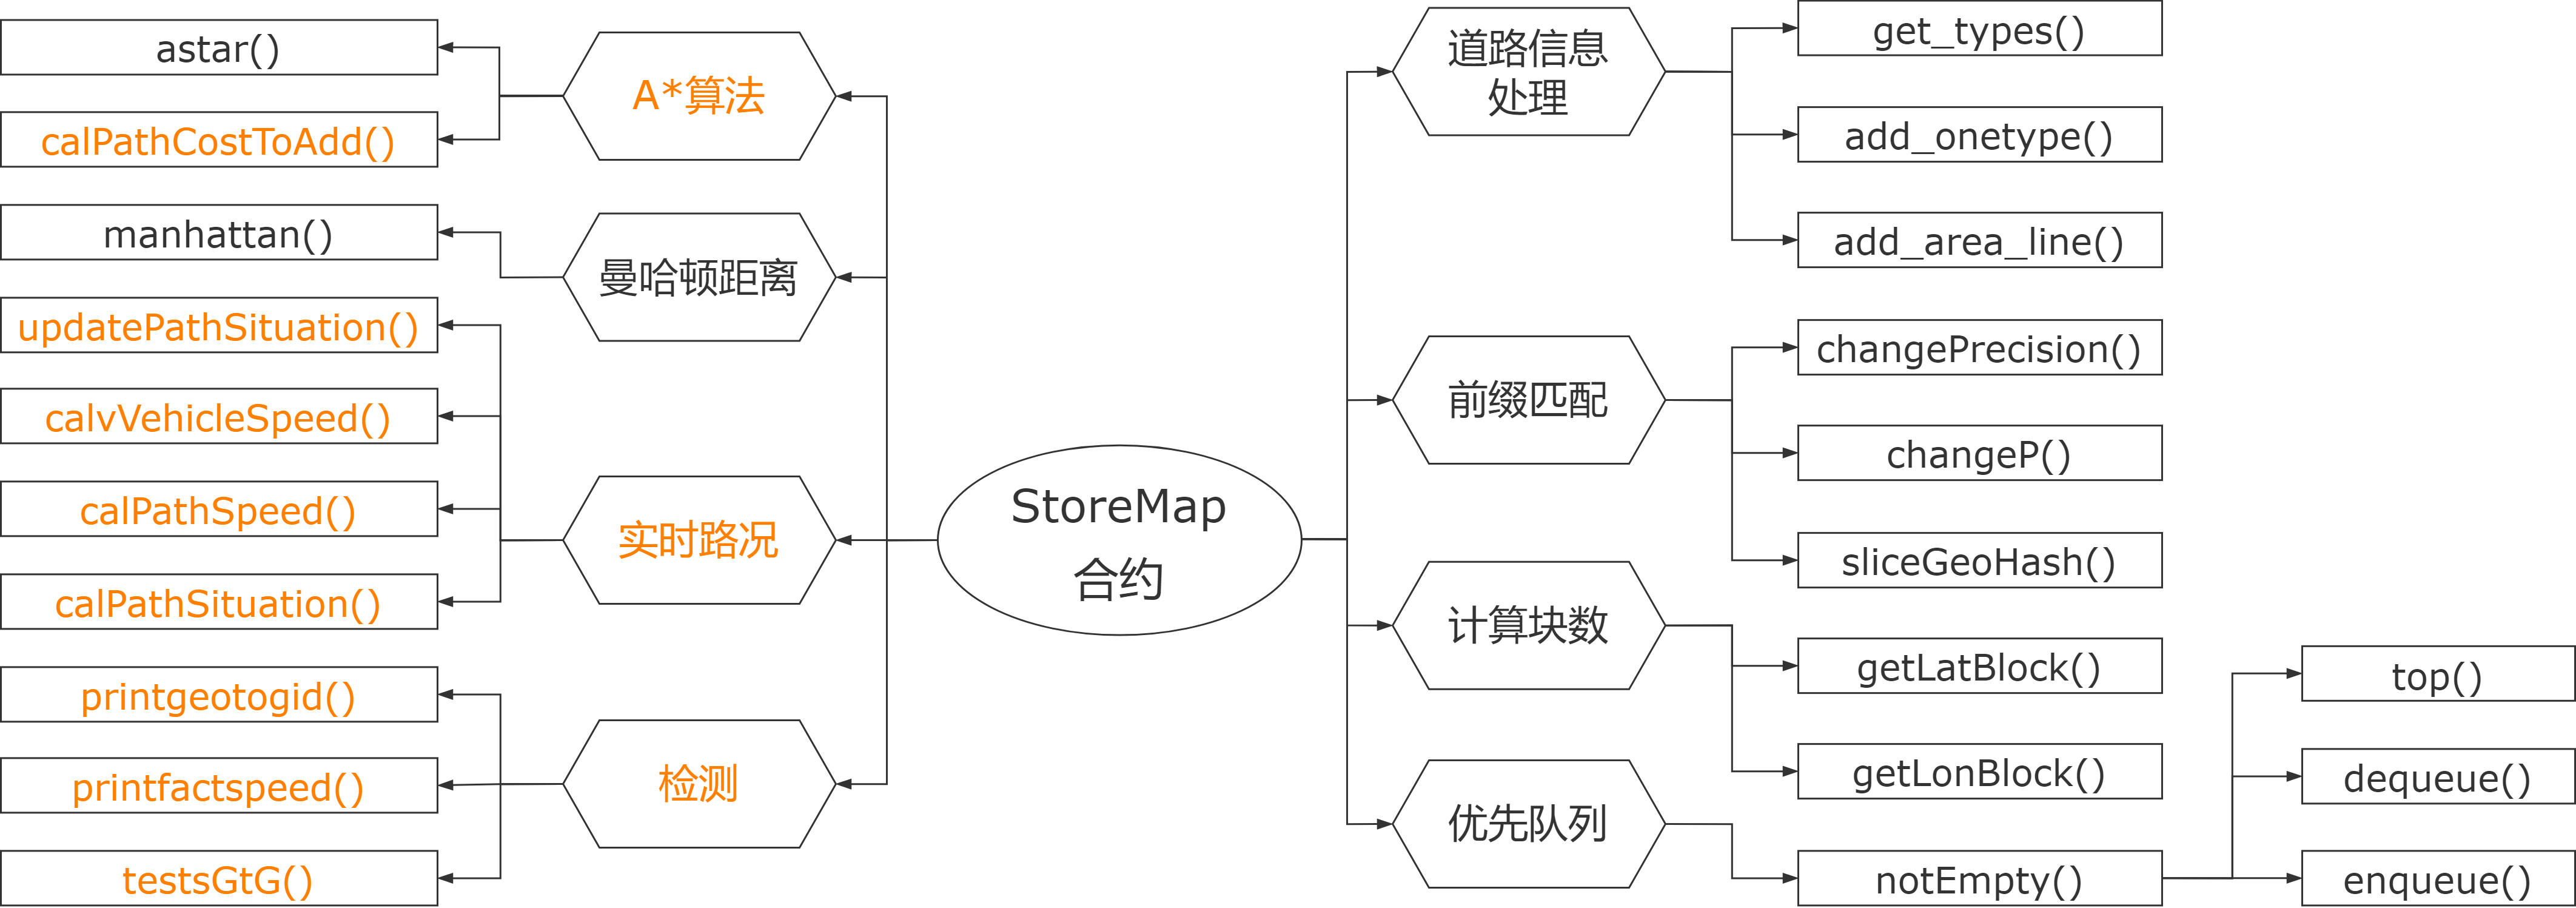
\includegraphics[width=1\textwidth]{undergraduate-thesis/images/StoreMapContract.png}
  \caption{StoreMap.sol架构示意图}
  \label{SMContract} % label 用来在文中索引
\end{figure}

本文将出租车调度系统中的寻路算法更新为结合实时路况的改进A*算法,主要做的修改是在智能合约StoreMap.sol中。图\ref{SMContract}是合约StoreMap.sol的架构示意图。黑色的函数对应的是合约中原有的函数,本文在其基础上,补充了计算实时路况、检测这两个模块;接下来,本文补充了calPathCostToAdd()函数,其归类在A*算法模块下,在同模块的astar()函数中调用,对总距离代价F的计算公式也做了对应修改;本文还补充了将Geohash值映射为路段gid值的mapping结构,在使用add\_onetype()存储路径时对其进行写操作,以方便用Geohash值对路段进行查询的读操作。

由于本文工作未对StoreTraffic.sol、Credit.sol进行修改,因此本文未对这两个合约的架构示意图进行分析展示。

本文所依赖的出租车调度系统有两种运行模式,一种是借助前端进行运行,在浏览器网页中,可以可视化看到向区块链里上传好的地图、A*算法规划完毕的路径、乘客和车辆不同时间段的状态、系统内部的某些变量等系统运行细节;另一种是借助控制台直接运行测试脚本,在控制台里,可以输出各环节乘客和车辆的不同状态、以Geohash编码的形式输出A*算法规划完毕的路径、输出系统内部的某些变量值,但无法可视化看到规划好的路径,可视化看到区块链中存储的地图。

但无论是借助前端运行还是借助控制台运行,本出租车调度系统与区块链中部署的智能合约的交互过程都是通过调用合约内容、向区块链提交交易完成的。两种运行方式的不同之处仅仅在于是否调用前端做出类似打车软件一样的可视化效果。因此,本文接下来将以借助前端运行的过程为例,阐明结合实时路况的改进A*算法应该如何在出租车调度系统中完成调用过程。
% 图得再改,改成能看清字的,只放函数名称得了
\begin{figure}[ht]
  \centering
  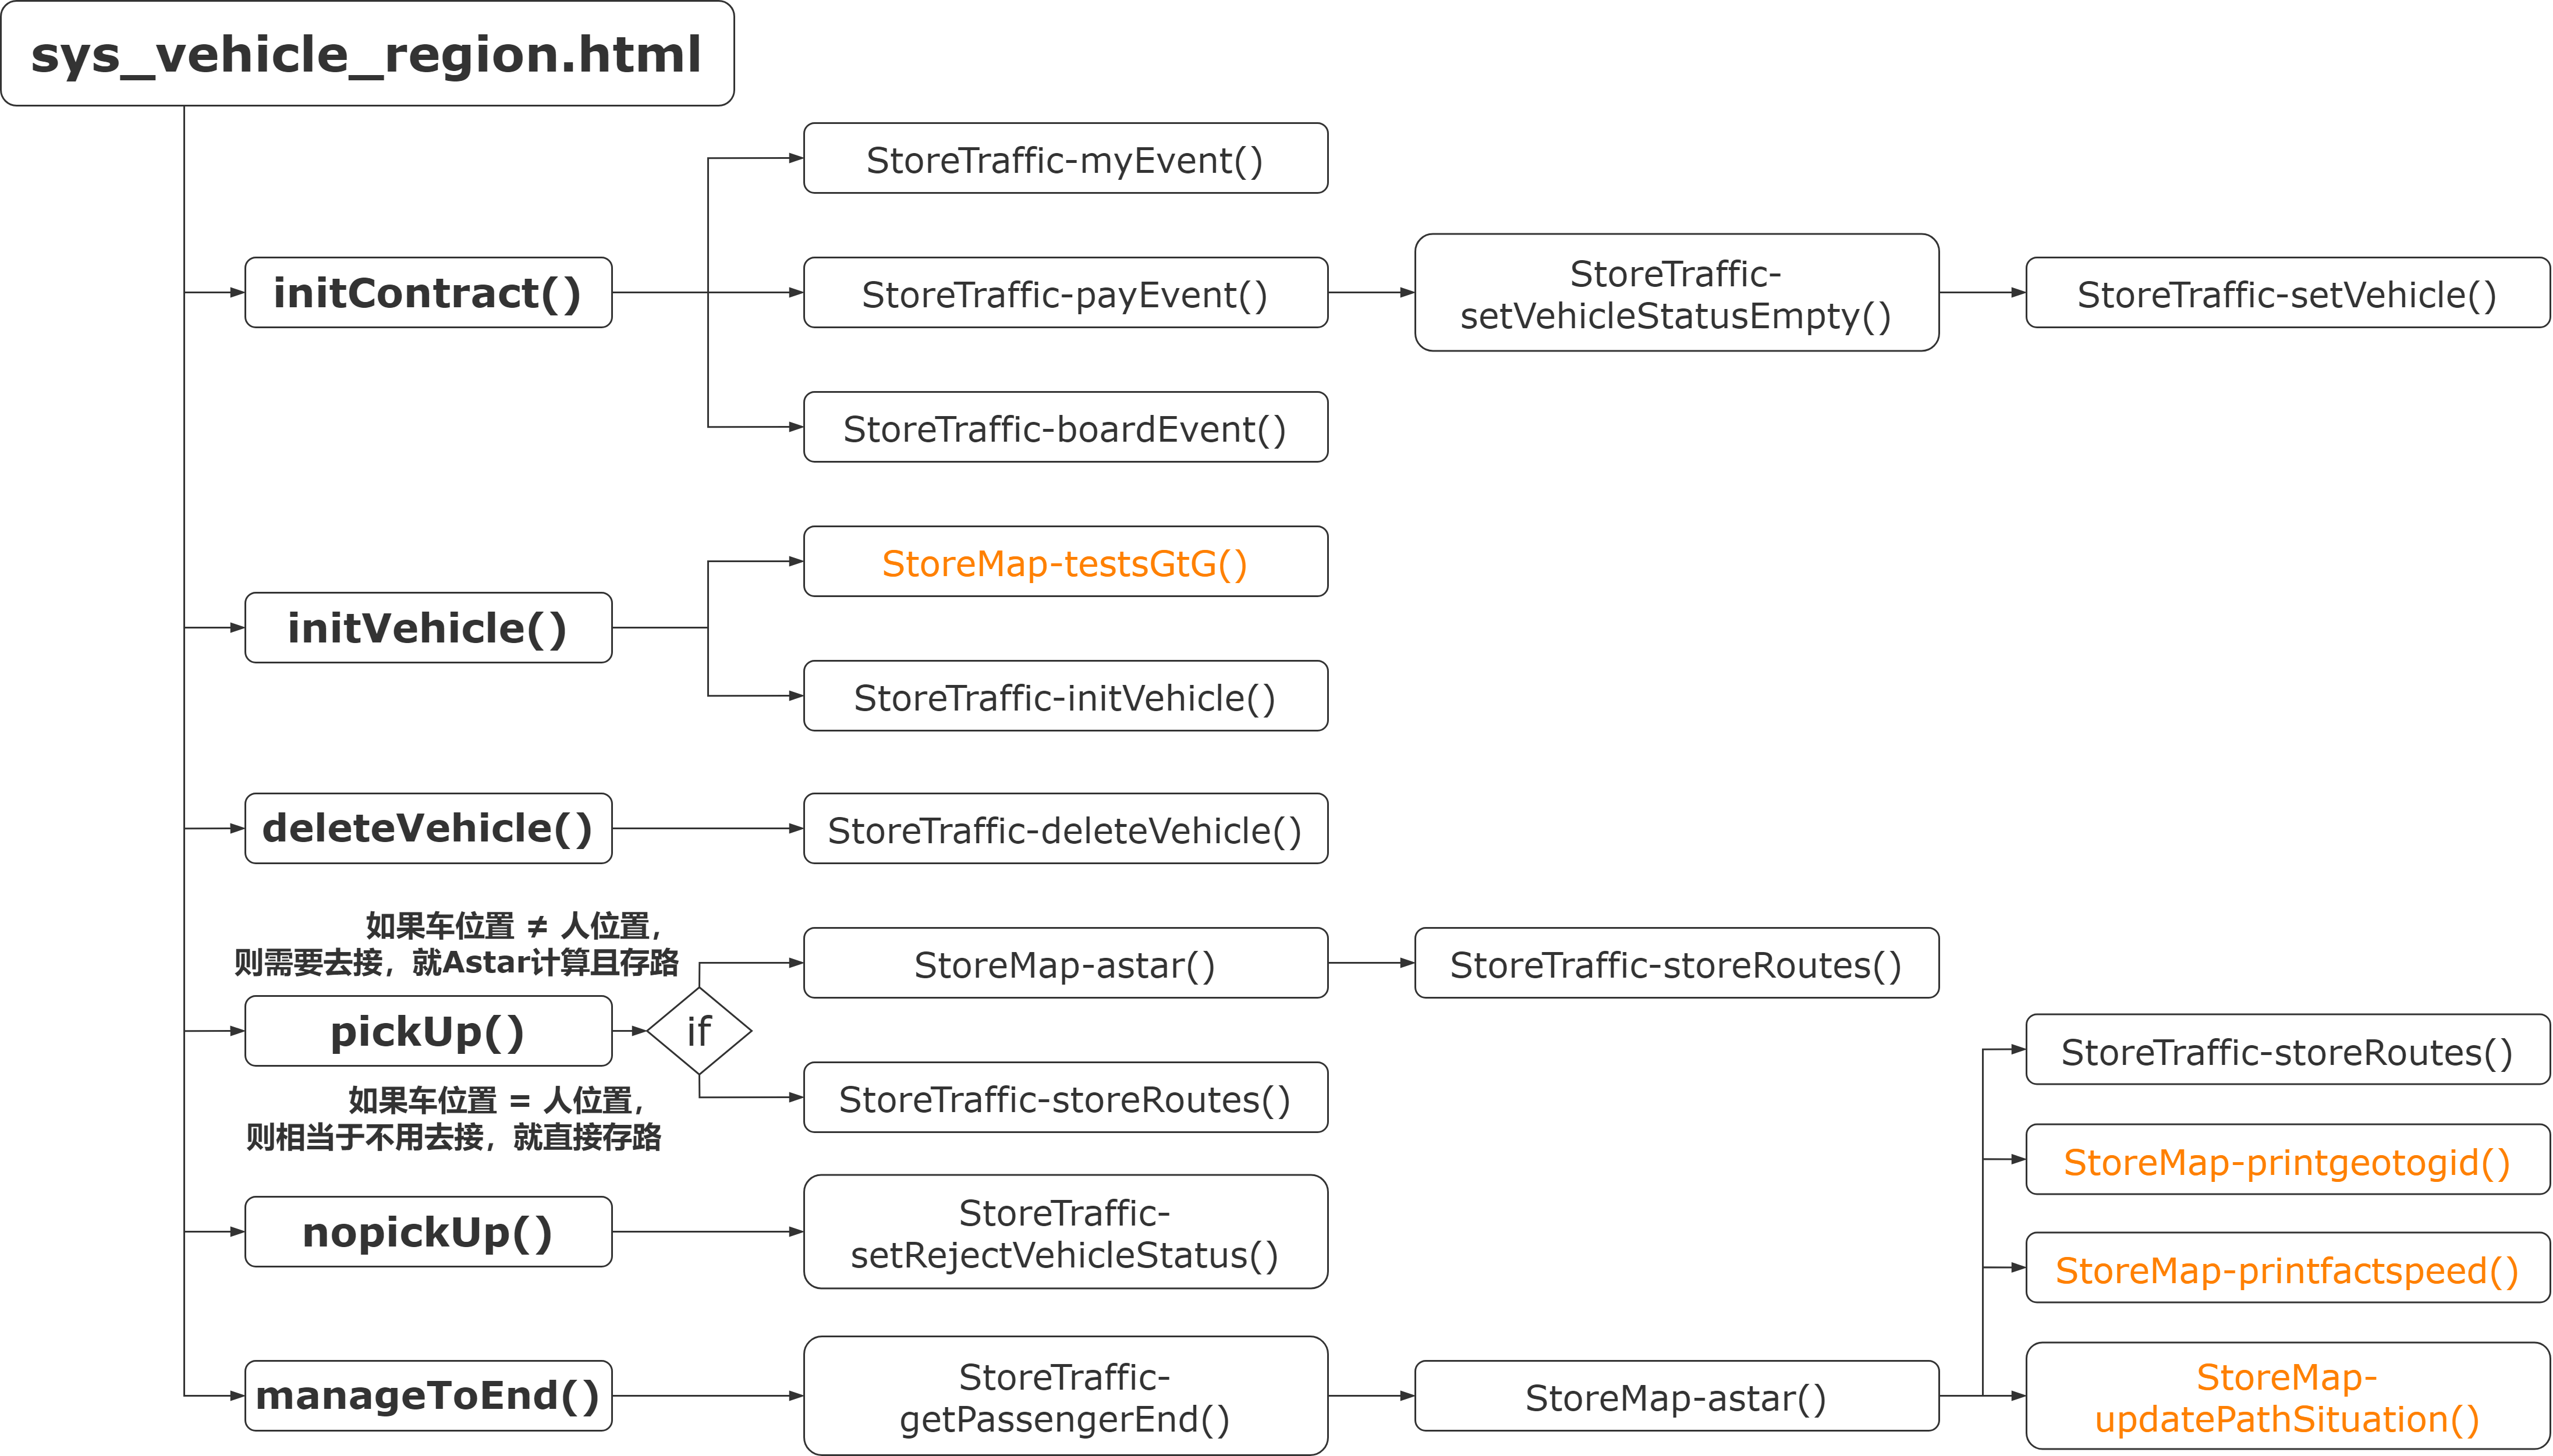
\includegraphics[width=1\textwidth]{undergraduate-thesis/images/callContracts_vehicle.png}
  \caption{车辆端Vehicle调用智能合约的逻辑示意图}
  \label{callContractsV} % label 用来在文中索引
\end{figure}

图\ref{callContractsV}展示了在出租车调度系统运行时,车辆端Vehicle所对应的前端网页调用智能合约的逻辑。它一共拥有6个主要的函数。黑色的合约函数是本系统中已有的,橙色的合约函数是本文为实现动态的路径规划而添加的调用过程。

1.initContract():初始化合约、监听前端事件发生。这个函数监听前端发生的乘客发起乘车请求、车辆接到乘客、乘客支付成功等事件,并根据事件种类调用不同函数。当MyEvent事件触发时,说明乘客发出订单,此时进行pickUp()过程,车辆由车辆位置前往乘客起点,在此期间需要使用合约中astar()函数进行一次动态路径规划;当boardEvent事件触发时,说明车辆已经接到乘客,此时进行manageToEnd()过程,车辆由乘客起点前往乘客终点,在此期间需要使用合约中astar()进行一次动态路径规划、使用合约中updatePathSituation()进行一次实时路况更新。

2.initVehicle():初始化车辆信息。它调用合约中initVehicle()来完成:上传车辆位置、初始化车辆状态的作用。本文在此函数中添加了对合约中testsGtG()函数的调用,目的是为了测试地图上传时,合约是否能正常存储Geohash到gid的映射关系。

3.deleteVehicle():删除车辆信息。系统每个轮次结束运行后,乘客到达终点并完成支付,车辆被认为完成此次运行,因此删除本轮次已经完成运行的车辆信息。

4.pickUp():接乘客过程模拟。该函数出现在系统运行的第一个重要阶段,此时乘客和车辆都已完成初始化,乘客发出了打车请求,并且通过区块链完成对车辆的呼叫,车辆接单,此时通过pickUp()来完成从车辆的初始位置运行到乘客的起点,实现接到乘客的效果。该过程主要调用合约内astar()函数,astar()函数规划一条以车辆位置为起点、以乘客起点为终点的道路。

5.nopickUp():车辆拒接乘客。该函数调用合约中setRejectVehicleStatus()函数来完成拒接效果。

6.manageToEnd():送乘客过程模拟。该函数出现在系统运行的第二个重要阶段,此时车辆已接到乘客。此过程调用合约中astar()函数,通过区块链完成动态路径规划,给出从乘客起点到乘客终点的行驶路径,从而完成乘客此次订单,并调用合约中updatePathSituation()函数完成对当前轮次运行过程的实时路况的计算,并将该计算结果存进区块链。

由于基于实时路况的改进A*算法在出租车调度系统里只在车辆Vehicle端被调用,在实现改进的A*算法的过程中不需要对乘客Passenger端的合约调用逻辑进行修改,因此本文未对乘客Passenger端的合约调用逻辑进行分析展示。

\section{本章小结}

首先,本章介绍了基于区块链的出租车调度系统的整体结构。

接着,本章从传统A*算法的公式引入,介绍了传统A*算法所依赖的总距离代价函数F(n)的计算方式。F(n)由耗散函数G(n)和启发函数H(n)构成,G(n)的计算过程和结果一般固定,但启发函数H(n)有不同的计算方式,且选取不同方式得出的计算结果会存在差异。结合本系统向区块链上传的地图特性与出租车调度系统是基于城市横平竖直的街道运行的特点,本文最终选取曼哈顿距离作为A*算法的启发函数H(n)进行计算。接下来,本章结合传统A*算法的流程图和简单的例子,对传统A*算法规划路径整体过程进行了阐述。随后,本章根据A*算法的特性给出了设计结合实时路况的改进A*算法的必要性。

本章在第\ref{A*New}节从计算实时路况、改进A*算法总距离代价计算公式的两个环节阐明了改进A*算法的思路与过程,并强调了在计算实时路况时要注意影响因子的选取结果,接下来借助第\ref{A*Reason}节中的情景,描述了结合实时路况的改进A*算法的路径规划过程和预期效果。

最后,通过分析智能合约的实现逻辑、出租车调度系统与区块链交互时调用智能合约的逻辑,本章在第\ref{section_useNewAstarinTaxiSystem}节中给出了改进A*算法在出租车调度系统中的具体实现方法,并对出租车调度系统调用A*算法的整体逻辑进行了介绍。
\chapter{综合实验}

本章首先对第\ref{chapter-Data}章中获取的地图数据正确性进行了分析验证,以确保上传给区块链的真实地图数据可信。接下来以基于树状区块链的出租车调度系统为载体进行综合实验。经过本文工作完善后的出租车调度系统能够根据路况动态地规划路径,表明了本文提出算法的可应用性;在实验过程中获取的数据证明了结合实时路况的改进A*算法具有良好的时间复杂度与空间复杂度,证明了把基于实时路况的改进A*算法引入出租车调度系统这一行为具有可行性。

在本章的实验中,区块链服务端和客户端均部署在虚拟机内,配置环境为:

1.虚拟机软件:7.0.6版本的VirtualBox

2.虚拟机的Linux操作系统:22.04版本的Ubuntu。

3.虚拟机基础配置:(1)内存大小为5220MB;(2)4核处理器;(3)磁盘空间为30.00G。

本章实验中所对应的数据文件存放的Github地址见附录D。

\section{地图数据的正确性验证}

本文在第\ref{chapter-Data}章中一共准备了五份地图,分别为out\_wx4e.json、out\_wx4eq.json、out\_wx4er.json、out\_wx4en.json、out\_wx4ep.json。

由Geohash编码的特征可知,一个Geohash编码父区域所对应的Geohash值一定是该区域的子区域编码值的前缀。本文导出的五份地图中,out\_wx4e.json是out\_wx4eq.json、out\_wx4er.json、out\_wx4en.json、out\_wx4ep.json这四份子地图的父区域,每份子地图中含有几千条路段,每个路段会包含不同的经纬度点位,这些经纬度点位经由Geohash编码后,也以子地图区域的编码值为前缀。因此,定义以下四个名词:

\begin{enumerate}
    \item 数据总量:指当前地图文件中,所有Geohash编码数据的个数。
    \item 有效数据:指统计点位的Geohash值前缀与当前地图父区域的Geohash值相同的数据。此时认为该点位属于此地图父区域,该点位是有效数据。
    \item 无效数据:指统计点位的Geohash值前缀与当前地图父区域的Geohash值不同。此时认为该点位不属于此地图父区域,该点位是无效数据。
    \item 可信度:指在一份地图文件中,有效数据在数据总量中的占比。
\end{enumerate}

对五份地图数据中包含的点位进行统计,得到图\ref{mapdataanalysis-pic}中的结果,对该结果的解释和分析如下。

\begin{figure}[ht]
  \centering
  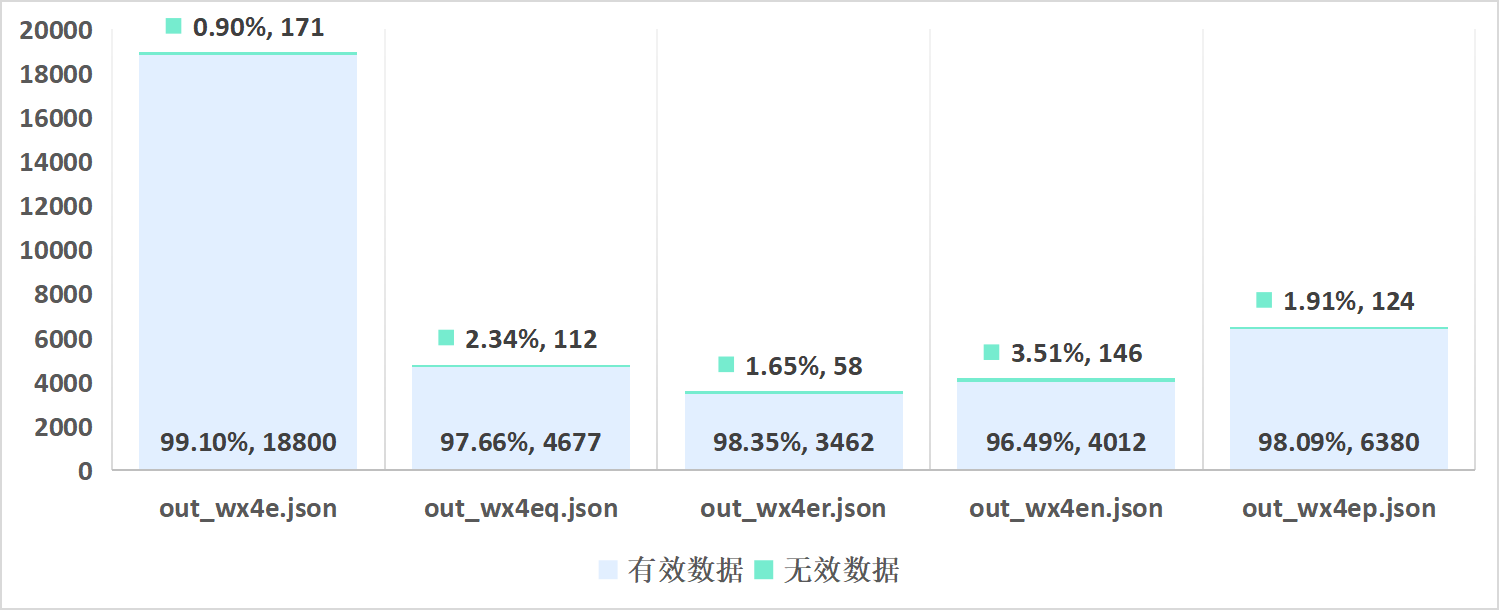
\includegraphics[width=0.9\textwidth]{undergraduate-thesis/images/mapDataAnalysis.png}
  \caption{第\ref{chapter-Data}章中有效地图数据占比图}
  \label{mapdataanalysis-pic} % label 用来在文中索引
\end{figure}

1.out\_wx4e.json地图:

此地图文件中:数据总量为18971;有效数据指以wx4eq、wx4er、wx4en、wx4ep为前缀的Geohash编码数据,其共有18800项,在数据总量中占比99.10\%;无效数据指以wx4g、wx4d、wx4ew、wx4em、wx4ej、wx4ex为前缀的Geohash编码数据,其共有171项,在数据总量中占比0.90\%。因此本地图文件可信度为99.10\%。

2.out\_wx4eq.json地图:

此地图文件中:数据总量为4789;有效数据指以wx4eq为前缀的Geohash编码数据,其共有4677项,在数据总量中占比97.66\%;无效数据指以wx4er、wx4em、wx4ew、wx4en为前缀的编码数据,其共有112项,在数据总量中占比2.34\%。因此本地图文件可信度为97.66\%。

3.out\_wx4er.json地图:

此地图文件中:数据总量为3520;有效数据指以wx4er为前缀的Geohash编码数据,其共有3462项,在数据总量中占比98.35\%;无效数据指以wx4eq、wx4ep、wx4ex、wx4g为前缀的编码数据,其共有58项,在数据总量中占比1.65\%。因此本地图文件可信度为98.35\%。

4.out\_wx4en.json地图:

此地图文件中:数据总量为4158;有效数据指以wx4en为前缀的Geohash编码数据,其共有4012项,在数据总量中占比96.49\%;无效数据指以wx4eq、wx4ep、wx4ej、wx4d为前缀的编码数据,其共有146项,在数据总量中占比3.51\%。因此本地图文件可信度为96.49\%。

5.out\_wx4ep.json地图:

此地图文件中:数据总量为6504;有效数据指以wx4ep为前缀的Geohash编码数据,其共有6380项,在数据总量中占比98.09\%;无效数据指以wx4er、wx4en、wx4g、wx4d为前缀的编码数据,其共有124项,在数据总量中占比1.91\%。因此本地图文件可信度为98.09\%。

\begin{figure}[ht]
  \centering
  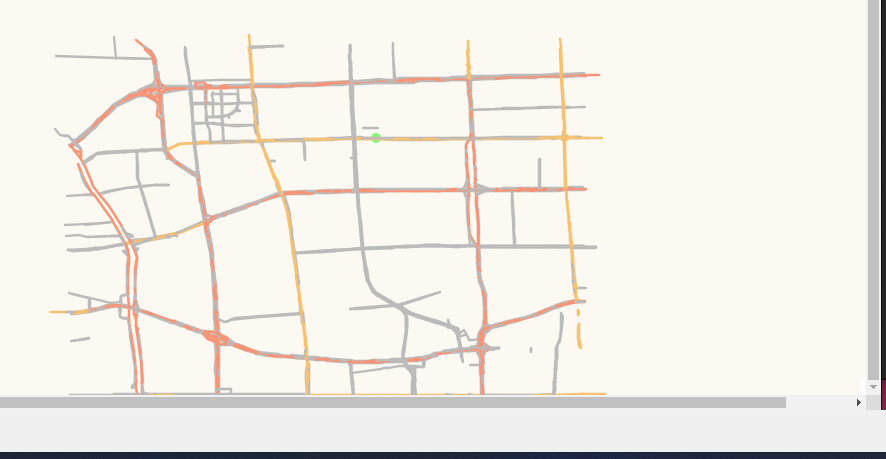
\includegraphics[width=0.8\textwidth]{undergraduate-thesis/images/2023-05-16 (7).png}
  \caption{out\_wx4e.json地图可视化效果}
  \label{wx4esuccess} % label 用来在文中索引
\end{figure}

由数据分析可知,五份地图文件的可信度分别依次为99.10\%、97.66\%、98.35\%、96.49\%、98.09\%。因此,认为第\ref{chapter-Data}章中给出的地图文件是正确可信的。

向系统中导入out\_wx4e.json数据后,其可视化效果如图\ref{wx4esuccess},证明本文中获取地图数据的过程是正确的;以out\_wx4eq.json地图数据为基础,在调度系统中完成一轮运行的成功图像如图\ref{wx4eqsuccess}所示,证明本文导出的地图数据能支持调度系统运行。

\begin{figure}[ht]
  \centering
  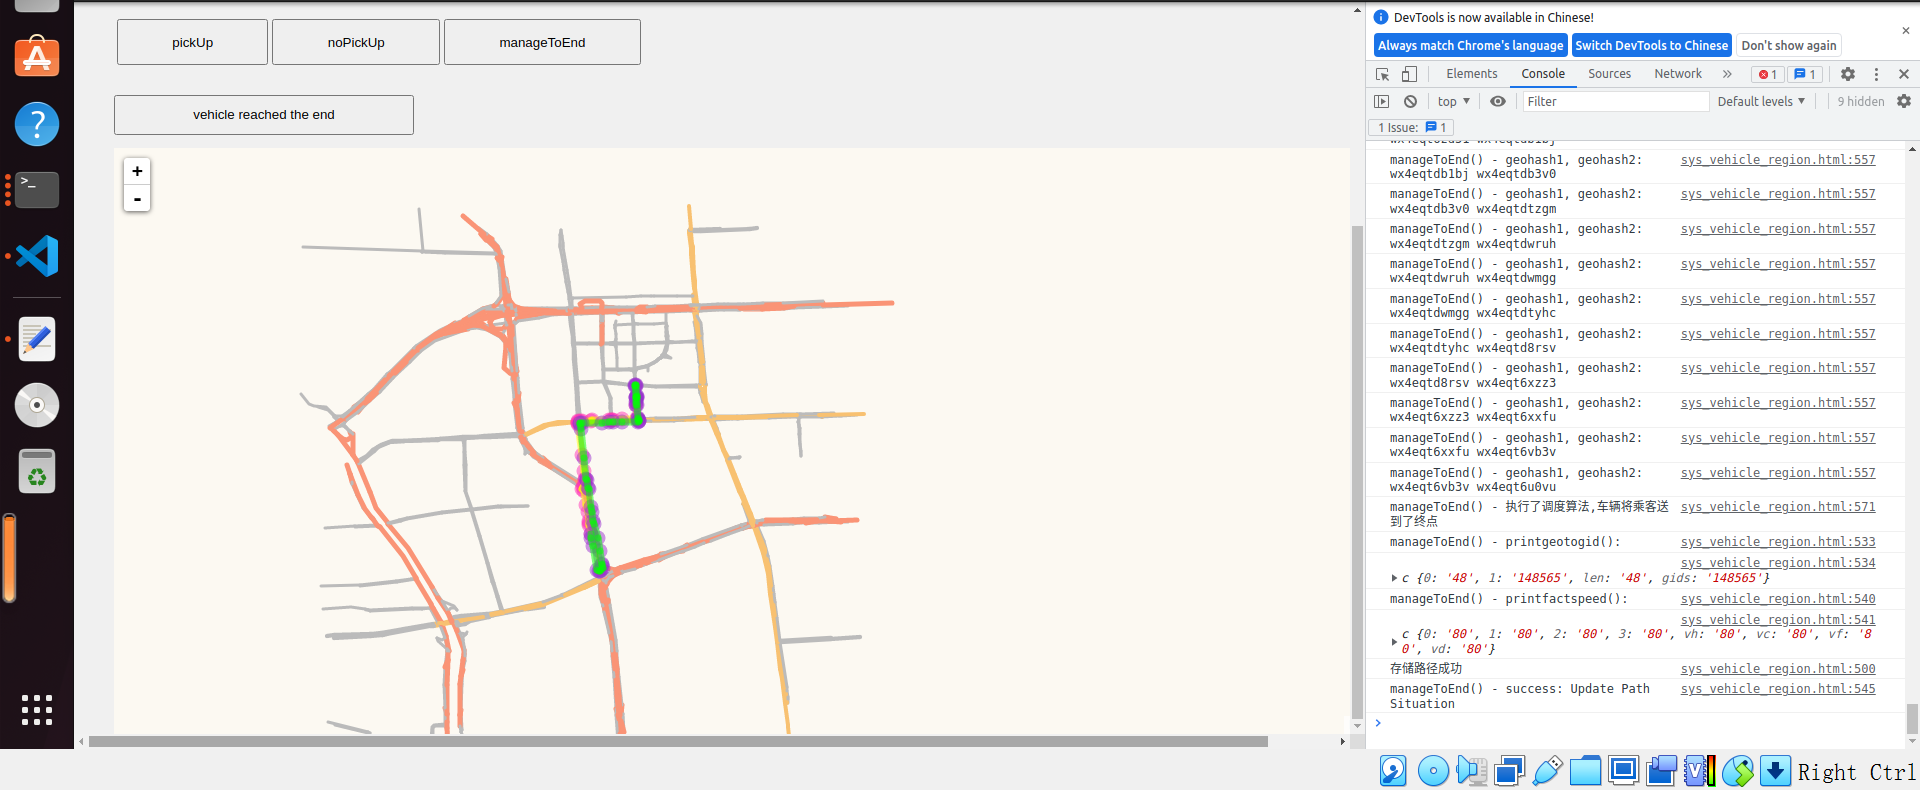
\includegraphics[width=0.9\textwidth]{undergraduate-thesis/images/2023-05-16 (12).png}
  \caption{out\_wx4eq.json上的运行效果}
  \label{wx4eqsuccess} % label 用来在文中索引
\end{figure}


\section{运行实验}
\label{runEx}

本节使用树状区块链的单子链,在方格地图上进行了基于改进A*算法的出租车调度系统的运行实验。

在本实验中,使用的车辆初始位置为:wx4erjmbekd(用绿色圆形标注);采取的乘客起点位置为:wx4erxjzekd(用蓝色圆形标注);采取的乘客终点位置为:wx4erjmbekd(用红色圆形标注)。在运行过程中,传统A*路径规划算法一共被调用2次,第1次是pickUp()过程,车辆从初始位置前往乘客起点,用黄色线条表示路径;第2次是manageToEnd()过程,车辆从乘客起点前往乘客终点,用绿色线条表示路径。

\subsection{使用传统A*算法的调度系统运行结果}

\begin{figure}[ht]
  \centering
  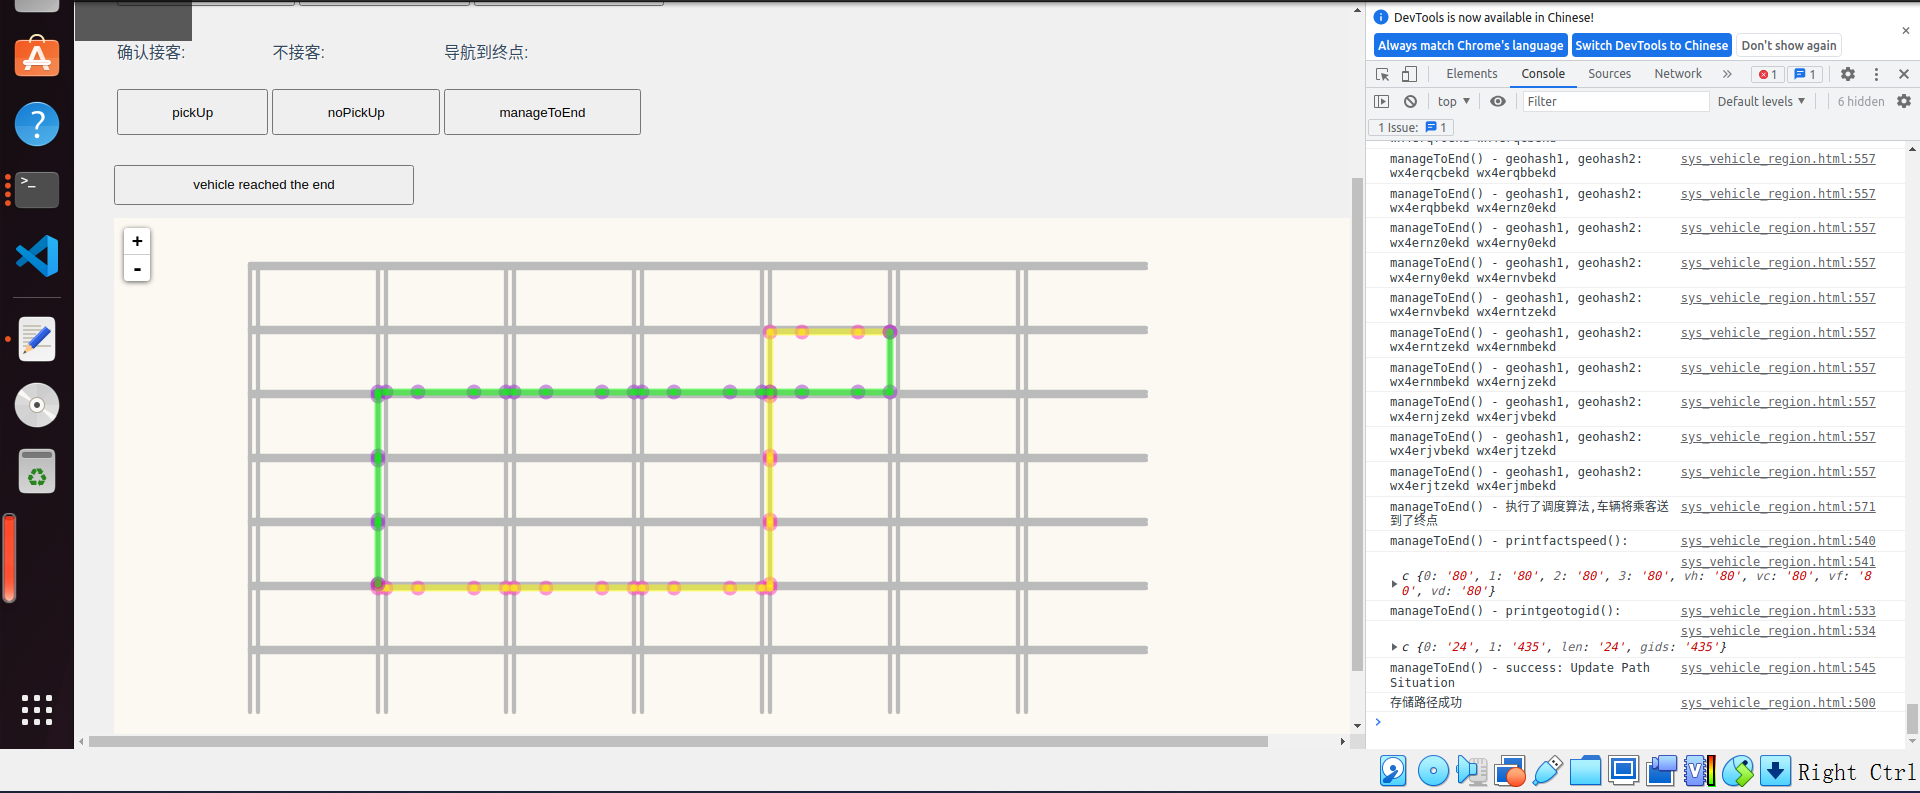
\includegraphics[width=0.9\textwidth]{undergraduate-thesis/images/2023-05-16 (1).png}
  \caption{使用传统A*算法的调度系统运行结果}
  \label{nine-old-Taxi} % label 用来在文中索引
\end{figure}

图\ref{nine-old-Taxi}中在pickUp()阶段和manageToEnd()阶段的总距离代价分别为3107和3069,这两个阶段规划出的结果如附录中的表\ref{exper1}所示。

使用传统A*算法的调度系统不考虑路况信息,只考虑道路距离,因此,无论运行多少次,只要区块链上部署的地图、车辆位置、乘客起点终点保持不变,则调度系统规划的黄色pickUp()路径和绿色manageToEnd()路径不会发生变化。

\subsection{使用改进A*算法的调度系统运行结果}

本文在智能合约中基于实时路况对A*算法完成了改进。在改进A*算法应用进出租车调度系统时,本文在智能合约与终端中进行以下假设:

1.路段的缺省速度为$V_{default}=80$km/h;

2.路段在第一次更新实时路况时保持通畅,即保持$V_{Current,1}=80$km/h。

3.在第n次更新实时路况时,如果有车辆在manageToEnd()阶段驶过某路段,将设定该路段的$V_{Current,n}=40$km/h,其中,$n\ge 2$。

4.在使用calPathCostToAdd()计算路段的实时路况代价时,设定公式\ref{cal-C(n)}中$\beta=15$,此举为了有效增加路段的实时路况代价,从而让运行结果有快速且明显的变化。

5.每轮运行一辆车、一位乘客,乘客发出一个订单,乘客完成支付、订单结束,则系统的本轮运行结束。

6.车辆位置、乘客的起点终点在不同轮次之间保持不变,此举的目的是能观察到不同轮次的实时路况对同一组位置的道路规划过程进行影响的变化效果。

基于以上六条假设,本系统进行了15轮运行,本文将对这15轮运行的结果从路况、道路成本代价两方面进行分析,并给出代表性的运行效果图。

\begin{figure}[ht]
  \centering
  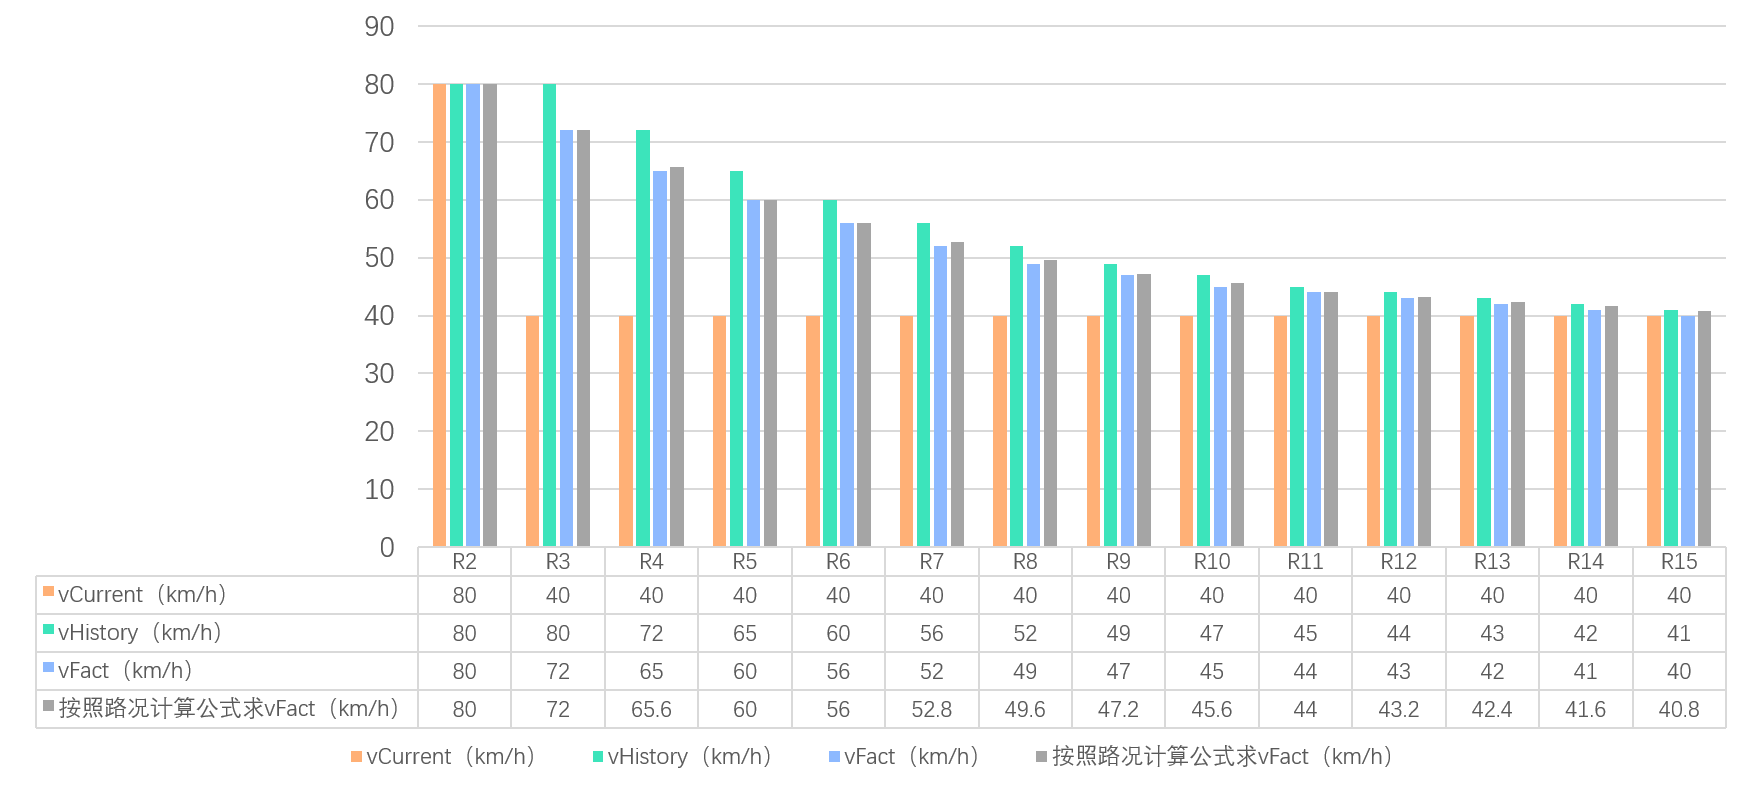
\includegraphics[width=1\textwidth]{undergraduate-thesis/images/PathSituationAnalysis.png}
  \caption{路况数据统计图}
  \label{nine-new-Taxi-path} % label 用来在文中索引
\end{figure}

图\ref{nine-new-Taxi-path}统计了第2轮次到第15轮次的道路速度数据,其中包括$V_{Current,n}$、$V_{History,n}$、$V_{Fact,n}$、$V_{default}$,由于$V_{default}$为道路的初始缺省速度,其一直保持不变,因此未在图\ref{nine-new-Taxi-path}中进行统计对比。

每次实时路况更新后,$V_{Current,n},(n\ge 2)$都为40,符合假设。

$V_{History,n}=V_{Fact,n-1}$,符合路况更新公式\ref{calpathSituation}。

根据公式\ref{calfact}:$V_{Fact,n}=V_{History,n}*0.8+V_{Current,n}*0.2$计算出的$V_{Fact,n}$如灰色数据所示,其与区块链上存储的数据$V_{Fact,n}$有较小差距。该差异出现的原因是:Solidity版本更新速度快,不同版本间的语法差异较大。本文使用的编译版本为0.5.17,该版本中的智能合约只能存储整数,不支持小数运算,因此在合约中实现公式\ref{calfact}时实际采用的计算公式为公式\ref{real-calfact},且计算出的$V_{Fact,n}$在区块链中只存储整数部分。
\begin{equation}
    V_{Fact,n}=(V_{History,n}*8+V_{Current,n}*2)/10
\label{real-calfact}
\end{equation}

数据证明,计算公式\ref{real-calfact}保留整数的效果较好,在无法存储小数的情况下能真实地逼近理想化的公式\ref{calfact}的计算结果,在区块链端进行数据存储。

\begin{figure}[!ht]
  \centering
  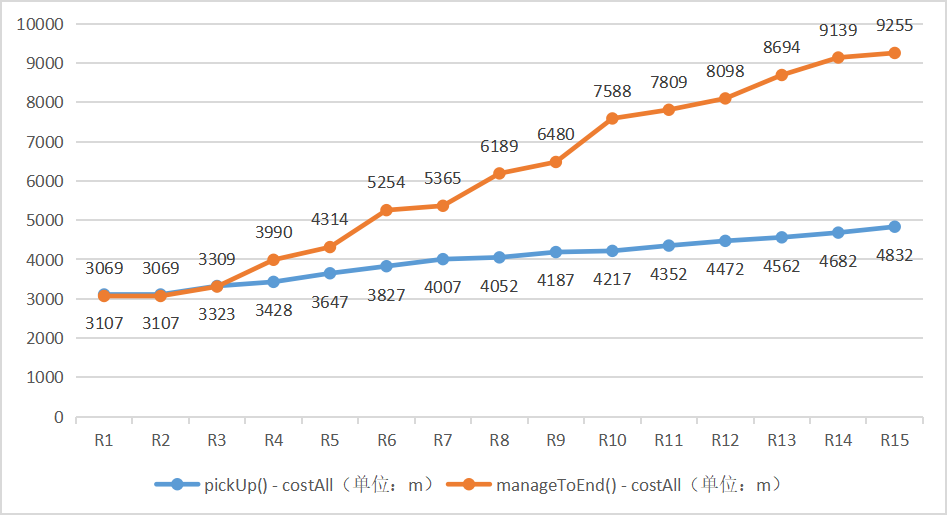
\includegraphics[width=1\textwidth]{undergraduate-thesis/images/CostAllAnalysis.png}
  \caption{改进A*算法在路径规划过程中的总距离成本数据统计图}
  \label{nine-new-Taxi-cost} % label 用来在文中索引
\end{figure}

本系统的调度过程分为两个阶段,第一个阶段是pickUp()过程,第二个阶段是manageToEnd()阶段。第一个阶段对车辆位置与乘客起点间进行路径规划,不调用updatePathSituation()更新实时路况,第二个阶段对乘客起点与乘客终点间进行路径规划,调用updatePathSituation()更新实时路况。costAll用于表示A*算法在路径规划过程中的总距离成本。在使用传统A*算法的调度系统的运行过程中,costAll和规划路径永远不变;在使用改进A*算法的调度系统的运行过程中,它的变化过程如图\ref{nine-new-Taxi-cost}所示。

在合约模拟道路速度的部分,只限定了路况拥堵状态,即车辆的运行导致路况从通畅变为拥堵,并未设计模拟道路由拥堵变成通畅的过程,因此costAll只会增加。pickUP()和manageToEnd()的costAll自第2轮开始都单调递增,这符合合约中模拟用例的预期效果。

pickUP()和manageToEnd()过程的costAll增长幅度不一致,前者增长速度缓慢且均衡,后者增长得越来越快。原因在于pickUp()过程未更新实时路况,其总距离成本costAll只会在manageToEnd()过程中走过的地方增加,增加的路段数量少,因此pickUp()的costAll增长慢且均匀。manageToEnd()每运行一次就会对此过程规划的每一段路段都增加拥堵效果,因此每运行一次,就会将该路段上所有位置的实时路况代价提高,提高的区域多,所以costAll增长比较快速。符合合约中模拟用例的预期效果。

\begin{figure}[!ht]
  \centering
  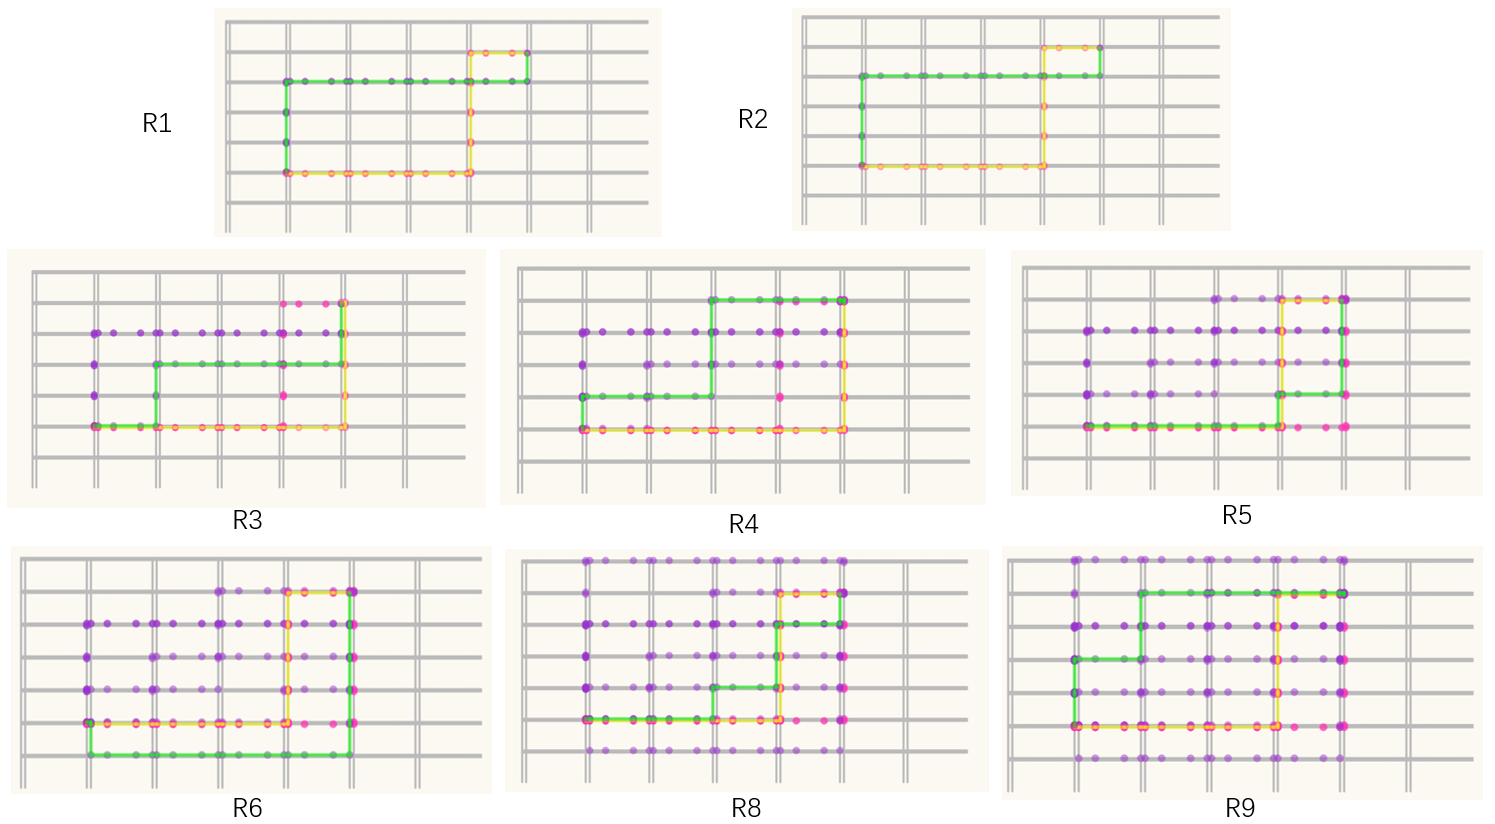
\includegraphics[width=1\textwidth]{undergraduate-thesis/images/2023-05-17.png}
  \caption{使用改进A*算法的调度系统运行结果示例}
  \label{nine-new-Taxi-pic1} % label 用来在文中索引
\end{figure}

图\ref{nine-new-Taxi-pic1}给出了本系统第1、2、3、4、5、6、8、9轮运行过程中的截图,该图中存在不同颜色的标识,各标识含义如下:黄色路径为pickUp()过程给出的路径规划结果;绿色路径为manageToEnd()过程给出的路径规划结果。黄色路径与绿色路径在路径规划结束后出现,在本轮订单完成后消失。粉色点线是pickUp()驶过的所有路径,紫色点线是manageToEnd()驶过的所有路径。当黄色路径出现时,粉色点线同时出现;当绿色路径出现时,紫色点线同时出现。车辆浏览器终端保持开启的时间段内,粉色点线和紫色点线不会消失;车辆浏览器终端重启,则粉色点线和紫色点线随之清零,并从零开始显示。设计不同颜色的路线,主要用于对比路径规划结果的区别。用粉色和紫色点线代表旧的路径规划路线结果,用黄色和绿色线段代表本轮的新路径规划路线结果,可视化表明第n轮规划出的新路线与第n-1轮规划出的旧路线基于实时路况发生变化。

在图\ref{nine-new-Taxi-pic1}中,由于$R1$、$R_2$轮次中道路路况均保持通畅,因此这两轮的calPathCostToAdd()计算结果都为0,则此两轮运行时,实时路况对道路规划的结果存在影响,但由于道路通畅,所以不改变道路规划结果。在$R_2$轮次结束之后,每轮运行都会使道路出现拥堵状况,因此实时路况会改变道路规划结果,新路径规划结果所对应的总距离成本代价值costAll在图\ref{nine-new-Taxi-cost}中得到统计,规划出的新路径在图\ref{nine-new-Taxi-pic1}中可视化表现。粉色、紫色路径在之前轮次被选出后,附加了道路拥堵状态,因此新轮次中如果继续按照粉色、紫色路径运行,道路成本将会升高,所以改进A*算法会规划出与其不同的黄色、绿色路径,作为道路成本最低的新路径,供车辆行驶。

%总结一下实验的结论,强调一下实验结果

在传统A*算法的控制下,本系统给出的路径规划结果只关注路径长度这一个因素,因此永远不变,其寻得路径如图\ref{nine-old-Taxi}所示,该路径规划结果中包含的Geohash编码如附录C中表\ref{exper1}所示;在改进A*算法的控制下,本系统给出的路径规划结果关注实时路况与路径长度这两个因素,由于实时路况在不断变化,因此路径规划结果也会不断变化,这符合现实生活中司机根据当前道路拥堵而选择其他较通畅道路的场景。

\section{性能实验}
% ----- 更新实验
本节在第\ref{runEx}节的基础上,使用了与运行实验相同的地图数据和车乘位置数据,并采取了相同的区块链服务端部署方式,但在终端部分使用JaveScript脚本通过web3接口直接与智能合约进行交互,以便于统计数据。本实验连续运行50轮出租车调度系统,获取到了50组运行数据。本节对这50组数据从不同角度进行了分析,综合评价了改进A*算法在应用进出租车调度系统后的性能,验证了本文改进的调度系统的可行性。

本实验关注以下两个性能指标:更新实时路况的时间损耗、改进A*算法的复杂度。

\subsection{更新实时路况的时间损耗}

本小节分析了在方格地图上运行使用改进A*算法的出租车调度系统,更新实时路况的时间损耗数据。该时间损耗发生在从终端的测试脚本里调用合约中更新实时路况的整个过程中,本文统计了系统每一轮运行过程中,调用合约里更新实时路况的全过程用时,并采用系统每一轮运行中的其他阶段用时作为对比数据。

\begin{figure}[ht]
  \centering
  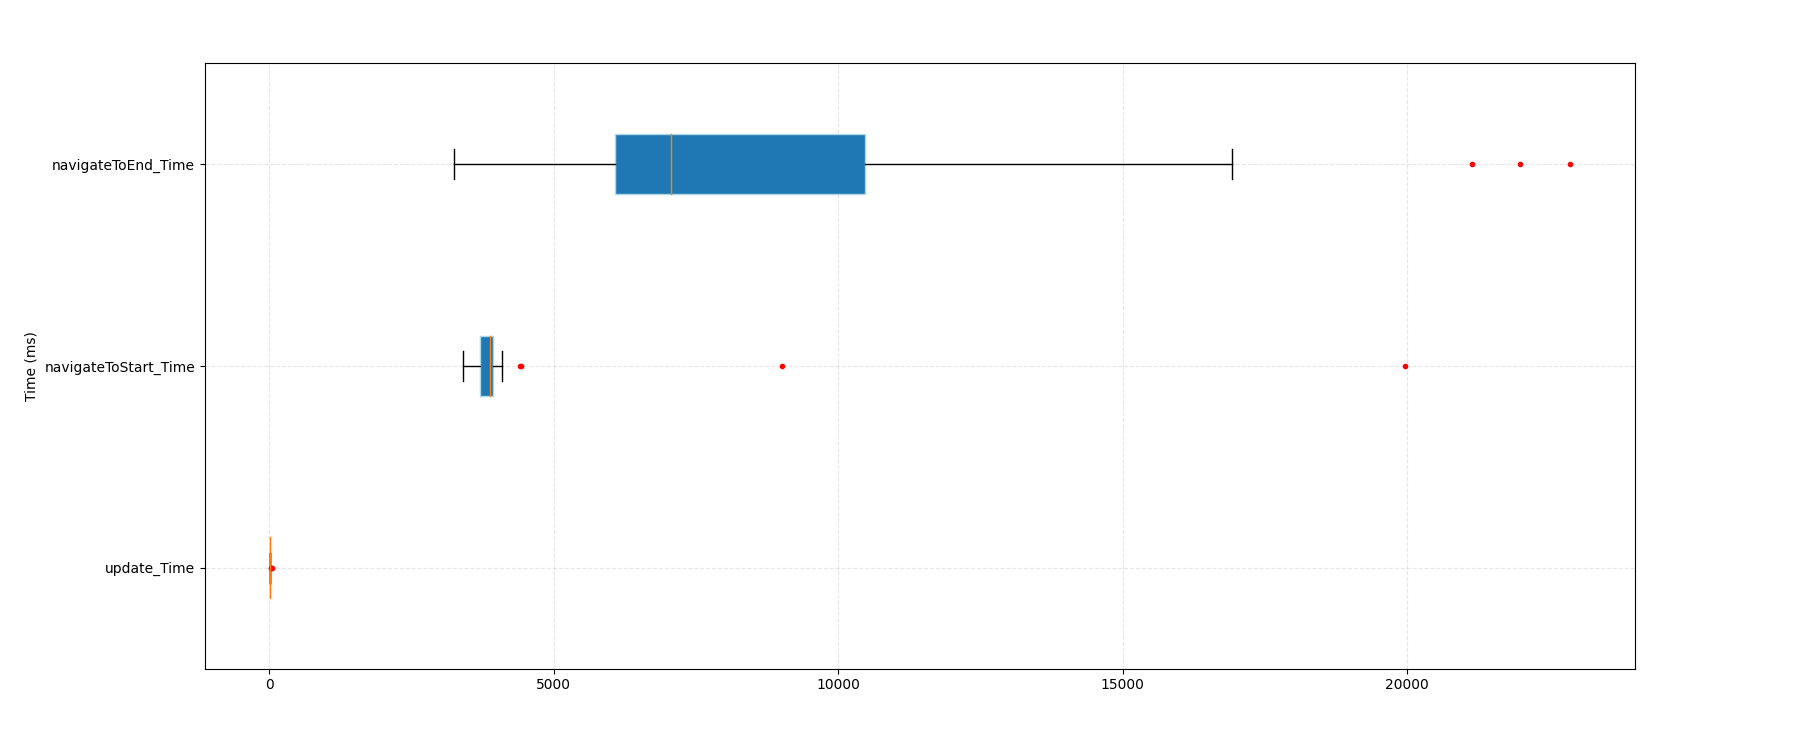
\includegraphics[width=1\textwidth]{undergraduate-thesis/images/2023-05-22 (2).png}
  \caption{系统运行不同阶段的时间损耗对比(单位:ms)}
  \label{nine-new-Taxi-time} % label 用来在文中索引
\end{figure}

图\ref{nine-new-Taxi-time}中展示了更新实时路况(update\_Time)、规划车辆前往乘客起点的路径(navigateToStart\_Time)、规划车辆从乘客上车到前往目的地的路径(navigateToEnd\_Time)这三个阶段的时间损耗数据,单位为ms。

update\_Time的中位数为10ms,平均值为10.82ms;navigateToStart\_Time的中位数为3882ms,平均值为4253.96ms;navigateToEnd\_Time的数据中位数为7225ms,平均值为8803.36ms。

可见,update\_Time的用时损耗占车辆前往乘客起点时间的0.25\%左右,占车辆接到乘客后前往乘客终点时间的0.13\%左右。在车辆通过智能合约规划路径时,需要借助合约中的A*算法进行路况调度,其借助区块链服务端的数据进行了大量运算,耗时较长;在车辆更新实时路况时,在区块链服务端中修改数据量较小,不需访问大量数据,因此耗时极短。

这说明,在基于树状区块链的出租车调度系统添加更新实时路况的环节后,该环节几乎不影响整个系统的运行时间,因此证明了本文所改进的实时路况计算部分具有极高的可行性。

\subsection{改进A*算法的复杂度}

\begin{figure}[ht]
  \centering
  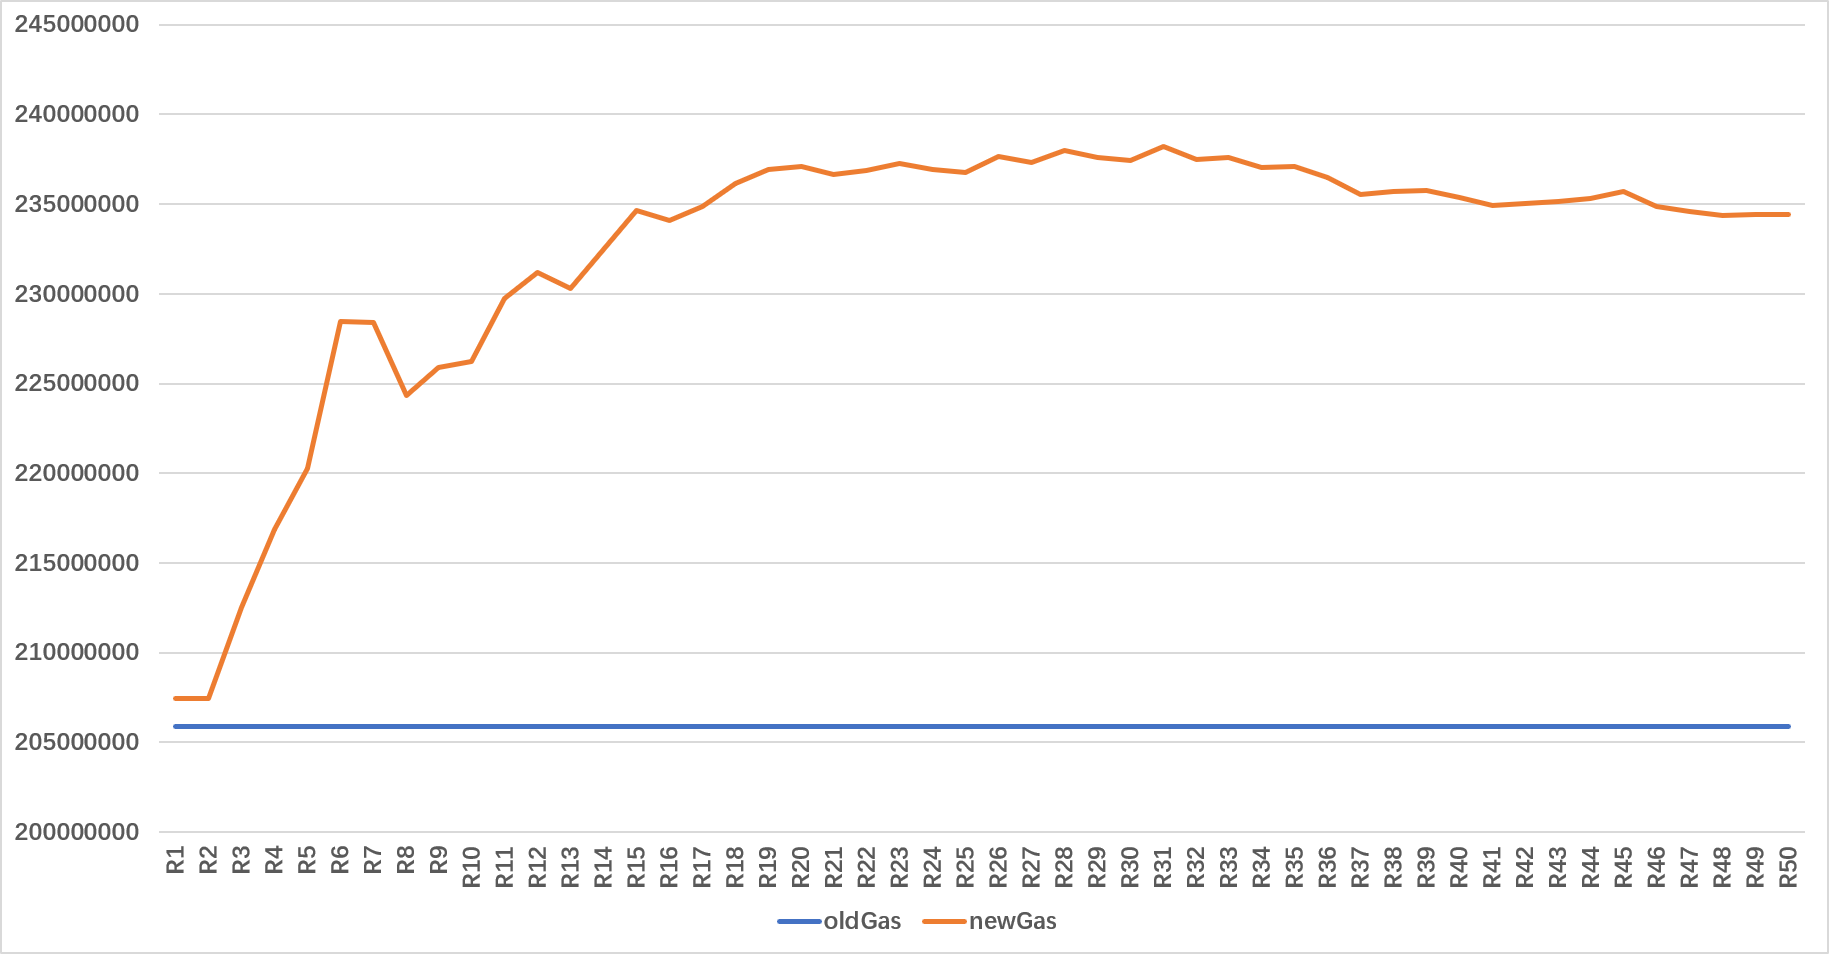
\includegraphics[width=0.8\textwidth]{undergraduate-thesis/images/gasData.png}
  \caption{改进前后A*算法的gas消耗}
  \label{nine-new-Taxi-gas} % label 用来在文中索引
\end{figure}

在区块链中,每笔智能合约的运行都需要支付一定量的gas,该gas的多少取决于智能合约的复杂度。因此,本节统计了智能合约运行过程中gas值的损耗量,用该数据量化代表A*算法的复杂度,对比传统A*算法消耗gas量与改进A*算法消耗gas量,作为改进A*算法的复杂度参考。

图\ref{nine-new-Taxi-gas}展示了传统A*算法和改进A*算法在被调用时消耗的gas量,oldGas线对应传统A*算法的gas损耗,newGas线对应改进A*算法的gas损耗。

该图像反映3个可关注信息:1. oldGas线为水平直线;2. newGas线整体高于oldGas线;3. newGas线整体的走势为增长趋势,且前半段爬升较快,后半段趋于稳定,以第$Round_{16}$轮次为界。对这些信息的分析如下:

\begin{enumerate}
    \item 图中oldGas线对应的数据为定值,在图像中表现为一条水平直线,这是因为:在使用传统A*算法的出租车调度系统运行过程中,由于传统A*算法只根据道路长度规划路径,因此每次的计算量是固定的,则算法复杂度也是固定的,量化为gas值损耗后,其gas损耗也为定值205910896,这符合图像中oldGas线的趋势。
    \item 图中newGas线整体高于oldGas线,这是因为:在使用改进A*算法的出租车调度系统运行过程中,由于改进A*算法将实时路况纳入计算因素,每轮规划完路径后会同步更新路况,因此区块链中存储的路况数据将不断增长,因此newGas线整体高于oldGas线,这证明改进A*算法的整体计算量和复杂度要高于传统A*算法。
    \item newGas线整体走势为增长趋势,且前半段变化剧烈,后半段趋于稳定,以第$Round_{16}$轮次为界,这是因为:(1)随着实时路况的计算,区块链中存储的数据不断增长,在调用改进A*算法时,对应的计算量也随之呈现整体上的增长趋势;(2)但根据计算,在第$Round_{15}$轮次路况更新结束之后,计算的$V_{fact,15}$已收敛到$V_{current,i}(i>=2)$对应的40km/h,因此区块链段更新的数据量较第$Round_{16}$轮以前有所减少,在调用改进A*算法时的计算量逐渐趋于稳定。该newGas线对应的数据符合智能合约中的行为及实时路况模拟行为,因此证明改进A*算法在本系统中运行合理且正常。
\end{enumerate}

在50轮的运行中,newGas的平均值为232461650.76,相比于oldGas来说提高了12.89\%。该数据说明在当前实时路况模拟的状态下,改进A*算法的复杂度较传统A*算法来说提高了12.89\%左右,该复杂度的提升尚可接受。相比于传统A*算法而言,改进A*算法提升了较低的复杂度,但能实现路径的动态规划效果,因此使用改进的A*算法对本文中提及的出租车调度系统进行完善是具有可行性的。

\section{本章小结}

首先,本章对本文处理的真实地图数据的正确性以统计的方式进行了分析与验证,以确保上传给区块链的地图数据符合北京道路特征,并且在系统中对真实地图数据进行可视化显示,保证了地图数据的可用性与正确性。

接着,本章使用方格地图数据,对使用传统A*算法的调度系统与使用改进A*算法的调度系统分别进行了运行实验与性能实验:1. 运行实验证明了改进A*算法在出租车调度系统中的可运行性。2. 性能实验的结果表明,结合实时路况的改进A*算法拥有良好的时间和空间复杂度,尽管改进A*算法相比于传统A*算法会提升一定的运算代价,但舍弃该代价能将路径规划由静态转为动态,更符合真实的出租车调度过程,为了模拟真实的调度场景,该代价是可接受的。本章的运行实验与测试实验证明了本文改善的出租车调度系统的可行性。

% \chapter{总结与展望}


% %%
% The BIThesis Template for Bachelor Graduation Thesis
%
% 北京理工大学毕业设计(论文)第二章节 —— 使用 XeLaTeX 编译
%
% Copyright 2020-2023 BITNP
%
% This work may be distributed and/or modified under the
% conditions of the LaTeX Project Public License, either version 1.3
% of this license or (at your option) any later version.
% The latest version of this license is in
%   http://www.latex-project.org/lppl.txt
% and version 1.3 or later is part of all distributions of LaTeX
% version 2005/12/01 or later.
%
% This work has the LPPL maintenance status `maintained'.
%
% The Current Maintainer of this work is Feng Kaiyu.
%%

\chapter{另一个章节}

\section{代码片段}

\begin{lstlisting}[language=Python, caption={Python Code}, label={lst:pythonfile}]
import numpy as np

def incmatrix(genl1,genl2):
    m = len(genl1)
    n = len(genl2)
    M = None #to become the incidence matrix
    VT = np.zeros((n*m,1), int)  #dummy variable

    #compute the bitwise xor matrix
    M1 = bitxormatrix(genl1)
    M2 = np.triu(bitxormatrix(genl2),1)

    for i in range(m-1):
        for j in range(i+1, m):
            [r,c] = np.where(M2 == M1[i,j])
            for k in range(len(r)):
                VT[(i)*n + r[k]] = 1;
                VT[(i)*n + c[k]] = 1;
                VT[(j)*n + r[k]] = 1;
                VT[(j)*n + c[k]] = 1;

                if M is None:
                    M = np.copy(VT)
                else:
                    M = np.concatenate((M, VT), 1)

                VT = np.zeros((n*m,1), int)

    return M
\end{lstlisting}

% \input{chapters/3_chapter3.tex}

% ---begin test
% \chapter{test-要删}

\section{代码插入测试}


% ---end test

% 后置部分
\backmatter

% 结论:在结论相应的 TeX 文件处进行结论部分的撰写
%%
% The BIThesis Template for Bachelor Graduation Thesis
%
% 北京理工大学毕业设计(论文)结论 —— 使用 XeLaTeX 编译
%
% Copyright 2020-2023 BITNP
%
% This work may be distributed and/or modified under the
% conditions of the LaTeX Project Public License, either version 1.3
% of this license or (at your option) any later version.
% The latest version of this license is in
%   http://www.latex-project.org/lppl.txt
% and version 1.3 or later is part of all distributions of LaTeX
% version 2005/12/01 or later.
%
% This work has the LPPL maintenance status `maintained'.
%
% The Current Maintainer of this work is Feng Kaiyu.
%
% Compile with: xelatex -> biber -> xelatex -> xelatex

\begin{conclusion}
汽车出行目前已成为我国社会的交通常态。相比于公交、地铁、传统打车方式而言,网约车方便用户预约车辆,实现点对点运输,完成对车辆的评价反馈,因此成为许多人首选的出行方式。网约车的兴起,满足了乘客个性化、便捷化的需求。但其数据处理、存储均通过第三方平台完成,依赖中心服务器,使数据安全无法得到保证。将区块链与车联网工作结合,保证司乘间可信交流,提升了打车平台的数据安全性,能营造更加高效且安全的打车服务。但目前已有的研究工作基于传统单链区块链,针对区块链节点在性能方面的处理效果进行优化,缺乏支持区域查询的树状区块链在实际业务应用场景的研究探索。且实验室前期设计实现的出租车调度系统使用静态的路径规划算法,无法模拟真实生活中的出租车调度场景。

针对上述问题,本文首先完成了对树状区块链技术的探索,针对Geohash编码技术与支持区域查询的树状区块链中的地理数据存储方式进行了分析,对传统A*算法与实时路况进行了研究。

接下来,本文基于实验室已有的研究,对已实现的基于传统A*算法的出租车调度系统进行了复现,形成了复现手册。在这一部分,本文还处理获取了较新的北京真实道路数据,将其整合为本系统所需的数据格式,部署到树状区块链上,完成了出租车调度系统中真实地图数据的导入工作。

接着,本文结合实验室早期对实时路况计算的研究,针对传统A*算法提出了基于实时路况的改进A*算法,并将其整合进出租车调度系统中,使车辆运行的路径能够在实时路况的影响下动态更换,从而更加符合真实应用场景。

最后,本文对该基于实时路况的改进A*算法进行了实验探究,以出租车调度系统为载体,分别完成运行实验与性能实验。运行实验证明了本文改进的出租车调度系统能在实时路况的影响下动态规划出更合适的通畅路段,从而说明了本文提出的算法的可运行性;性能实验证明了本文改进的A*算法在复杂度方面表现良好,证明了本文把基于实时路况的改进A*算法引入出租车调度系统的行为具有可行性。

% 不足与展望——
整体而言,本文工作完成了对出租车调度系统中道路规划算法的改进,通过结合北京真实地图数据、引入实时路况,在一定程度上模拟了真实场景中的出租车调度过程,为在基于树状区块链的出租车调度系统中实现完全真实的动态路径规划过程做出了探索,具有较高的实用价值。

但本文工作仍有可扩展的研究方向与不足之处:首先,实时路况计算的过程和方法仍待优化,如将车辆位置定时上传、考虑路口路况计算方式等。此外,通过完善信誉值模块的设计,促进司机与乘客之间的双向评价过程,提升车乘服务质量。最后,可以探索用户的身份认证机制,从而保证准入用户身份的真实性,加强系统安全性。

\end{conclusion}


% 参考文献:如无特殊需要,参考文献相应的 TeX 文件无需改动,添加参考文献请使用 BibTeX 的格式
%   添加至 misc/ref.bib 中,并在正文的相应位置使用 \cite{xxx} 的格式引用参考文献
%%
% The BIThesis Template for Bachelor Graduation Thesis
%
% 北京理工大学毕业设计(论文)参考文献 —— 使用 XeLaTeX 编译
%
% Copyright 2020-2023 BITNP
%
% This work may be distributed and/or modified under the
% conditions of the LaTeX Project Public License, either version 1.3
% of this license or (at your option) any later version.
% The latest version of this license is in
%   http://www.latex-project.org/lppl.txt
% and version 1.3 or later is part of all distributions of LaTeX
% version 2005/12/01 or later.
%
% This work has the LPPL maintenance status `maintained'.
%
% The Current Maintainer of this work is Feng Kaiyu.
%
% Compile with: xelatex -> biber -> xelatex -> xelatex
%
% 如无特殊需要,本页面无需更改

\begin{bibprint}
\printbibliography[heading=none]
\end{bibprint}

% 附录:在附录相应的 TeX 文件处进行附录部分的撰写
%%
% The BIThesis Template for Bachelor Graduation Thesis
%
% 北京理工大学毕业设计(论文)附录 —— 使用 XeLaTeX 编译
%
% Copyright 2020-2023 BITNP
%
% This work may be distributed and/or modified under the
% conditions of the LaTeX Project Public License, either version 1.3
% of this license or (at your option) any later version.
% The latest version of this license is in
%   http://www.latex-project.org/lppl.txt
% and version 1.3 or later is part of all distributions of LaTeX
% version 2005/12/01 or later.
%
% This work has the LPPL maintenance status `maintained'.
%
% The Current Maintainer of this work is Feng Kaiyu.
%
% Compile with: xelatex -> biber -> xelatex -> xelatex

\begin{appendices}
  % 这里示范一下添加多个附录的方法:
  % 使用 \section 来添加一个附录

\section{Geohash编码过程示例}

``北蜂窝路"的经度、纬度表示过程如以下两张表:

\begin{table}[!ht]
    \linespread{1.5}
    % \linespread{1.5}
    \zihao{5}
    \centering
    \caption{经度的二进制表示过程}
    \label{geohash-jingdu}
    \begin{tabularx}{\textwidth}{XXXc}
    \toprule
    纬度 & 划分区间0 & 划分区间1 & 116.3227718 \\
    \hline
    (-180,180) & (-180,0) & (0,180) & 1\\
    (0,180) & (0,90) & (90,180) & 1\\
    (90,180) & (90,135) & (135,180) & 0\\
    (90,135) & (90,112.5) & (112.5,135) & 1\\
    (112.5,135) & (112.5,123.75) & (123.75,135) & 0\\
    (112.5,\newline 123.75) & (112.5,\newline 118.125) & (118.125,\newline 123.75) & 0\\
    (112.5,\newline 118.125) & (112.5,\newline 115.3125) & (115.3125,\newline 118.125) & 1\\
    (115.3125,\newline 118.125) & (115.3125,\newline 116.71875) & (116.71875,\newline 118.125) & 0\\
    (115.3125,\newline 116.71875) & (115.3125,\newline 116.015625) & (116.015625,\newline 116.71875) & 1\\
    (116.015625,\newline 116.71875) & (116.015625,\newline 116.3671875) & (116.3671875,\newline 116.71875) & 0\\
    (116.015625,\newline 116.3671875) & (116.015625,\newline 116.19140625) & (116.19140625,\newline 116.3671875) & 1\\
    (116.19140625,\newline 116.3671875) & (116.19140625,\newline 116.279296875) & (116.279296875,\newline 116.3671875) & 1\\
    (116.279296875,\newline 116.3671875) & (116.279296875,\newline 116.3232421875) & (116.3232421875,\newline 116.3671875) & 0\\
    (116.279296875,\newline 116.3232421875) & (116.279296875,\newline 116.30126953125) & (116.30126953125,\newline 116.3232421875) & 1\\
    (116.30126953125,\newline 116.3232421875) & (116.30126953125,\newline 116.312255859375) & (116.312255859375,\newline 116.3232421875) & 1\\
    \bottomrule
    \end{tabularx}
\end{table}

% 设置三线表
\begin{table}[!ht]
    % \linespread{1.4}
    \linespread{1.5}
    \zihao{5}
    \centering
    \caption{纬度的二进制表示过程}
    \label{geohash-weidu}
    \begin{tabularx}{\textwidth}{XXXc}
    \toprule
    纬度 & 划分区间0 & 划分区间1 & 39.9037387 \\
    \hline
    (-90,90) & (-90,0) & (0,90) & 1 \\
    (0,90) & (0,45) & (45,90) & 0 \\
    (0,45) & (0,22.5) & (22.5,45) & 1 \\
    (22.5,45) & (22.5,33.75) & (33.75,45) & 1 \\
    (33.75,\newline 45) & (33.75,\newline 39.375) & (39.375,\newline 45) & 1 \\
    (39.375,\newline 45) & (39.375,\newline 42.1875) & (42.1875,\newline 45) & 0 \\
    (39.375,\newline 42.1875) & (39.375,\newline 40.78125) & (40.78125,\newline 42.1875) & 0 \\
    (39.375,\newline 40.78125) & (39.375,\newline 40.078125) & (40.078125,\newline 40.78125) & 0 \\
    (39.375,\newline 40.078125) & (39.375,\newline 39.7265625) & (39.7265625,\newline 40.078125) & 1 \\
    (39.7265625,\newline 40.078125) & (39.7265625,\newline 39.90234375) & (39.90234375,\newline 40.078125) & 1 \\
    (39.90234375,\newline 40.078125) & (39.90234375,\newline 39.990234375) & (39.990234375,\newline 40.078125) & 0 \\
    (39.90234375,\newline 39.990234375) & (39.90234375,\newline 39.9462890625) & (39.9462890625,\newline 39.990234375) & 0 \\
    (39.90234375,\newline 39.9462890625) & (39.90234375,\newline 39.92431640625) & (39.92431640625,\newline 39.9462890625) & 0 \\
    (39.90234375,\newline 39.92431640625) & (39.90234375,\newline 39.913330078125) & (39.913330078125,\newline 39.92431640625) & 0 \\
    (39.90234375,\newline 39.913330078125) & (39.90234375,\newline 39.9078369140625) & (39.9078369140625,\newline 39.913330078125) & 0 \\
    \bottomrule
    \end{tabularx}
\end{table}
% 结束设置三线表


\newpage

\section{使用SQL语句从postgreSQL中导出地图数据}

当已完成对表\ref{mapData_Addproperty}中的内容添加过程后,需要使用以下语句从数据库中将地图数据导出。该语句本质上是一套查询语句的嵌套过程,先按照筛选要求查询得到n条道路数据,再将这n条道路数据各自组合成n条区块链上所需的Json格式的数据,最后将这n条Json语句组合成一条Json语句。以下SQL代码段以导出wx4eq区域Json格式的地图数据为示例。

\begin{lstlisting}[language=sql, caption={导出wx4eq区域Json格式的地图数据}, label={lst:getmapdata}]
SELECT
  array_to_json(array_agg(row_to_json(ff)))
FROM
  (SELECT
    ( SELECT row_to_json(t) FROM
      ( select minzoom, fclass as highway, round(cost::numeric,0) as cost, gid, name, source, target, one_way as oneway ) 
      AS t 
    ) AS properties ,
    ST_AsGeoJSON(geom)::json AS geometry,
    'Feature' AS type 
  FROM bjway
  WHERE
    ((code = 5112 or code = 5113 or code = 5114 or code = 5115 or code = 5132 or code = 5133 or code = 5134 or code = 5135) and (start_x between 116.279 and 116.323) and (start_y between 39.947 and 39.991) and oneway = 'F') 
  order by gid) 
AS ff;\end{lstlisting}

\newpage

\section{方格地图上,传统A*算法规划的路径}
下表给出方格地图上,使用传统A*算法在出租车调度系统内运行出的路径规划结果。其中车辆初始位置为wx4erjmbekd,乘客起点为wx4erxjzekd,乘客终点为wx4erjmbekd。
% 设置三线表
\begin{table}[!ht]
    \linespread{1.5}
    \zihao{5}
    \centering
    \caption{传统A*算法给出的路径规划结果}
    \label{exper1}
    \begin{tabularx}{\textwidth}{p{3cm}X}
    \toprule
    阶段 & 路径规划结果 \\
    \hline
    pickUp() & wx4erjmbekd, wx4erjjzekd, wx4erjnpekd, wx4erjppekd\newline wx4erm0zekd, wx4erm1zekd, wx4erm4pekd, wx4erm5pekd\newline wx4ermhzekd, wx4ermjzekd, wx4ermnpekd, wx4ermppekd\newline wx4ert0zekd, wx4ert1zekd, wx4ert4pekd, wx4ert60ekd\newline wx4ertdpekd, wx4ertf0ekd, wx4erw4pekd, wx4erw60ekd\newline wx4erwdpekd, wx4erwf0ekd, wx4erx4pekd, wx4erx5pekd\newline wx4erxhzekd, wx4erxjzekd \\
    manageToEnd() &  wx4erxjzekd, wx4erwvbekd, wx4erwubekd, wx4erwg0ekd\newline wx4erwf0ekd, wx4erwcbekd, wx4erwbbekd, wx4erqz0ekd\newline wx4erqy0ekd, wx4erqvbekd, wx4erqubekd, wx4erqg0ekd\newline wx4erqf0ekd, wx4erqcbekd, wx4erqbbekd, wx4ernz0ekd\newline wx4erny0ekd, wx4ernvbekd, wx4erntzekd, wx4ernmbekd\newline wx4ernjzekd, wx4erjvbekd, wx4erjtzekd, wx4erjmbekd \\
    \bottomrule
    \end{tabularx}
\end{table}
% 结束设置三线表

在传统A*算法的控制下,只要地图不变,车辆位置、乘客起点与终点不变,无论系统运行多少次,规划出的路线都是上述路线,且该路线对应的总距离成本永远不变。

\newpage

\section{Github地址索引}

本文工作对应的Github仓库地址为:

\href{https://github.com/LancerEnk/GraduationDesign}{https://github.com/LancerEnk/GraduationDesign}

本文中提及的文件所在的仓库链接如下:
\begin{enumerate}
    \item \href{https://github.com/LancerEnk/GraduationDesign/blob/main/doc/\%E5\%A4\%8D\%E7\%8E\%B0\%E6\%89\%8B\%E5\%86\%8C/10\%20\%E9\%83\%A8\%E7\%BD\%B2\%E5\%9C\%A8geth-tree\%E4\%B8\%8A\%E7\%9A\%84\%E5\%87\%BA\%E7\%A7\%9F\%E8\%BD\%A6\%E8\%B0\%83\%E5\%BA\%A6\%E7\%B3\%BB\%E7\%BB\%9F\%E5\%A4\%8D\%E7\%8E\%B0\%E5\%AE\%9E\%E9\%AA\%8C.md}{第2章:树状区块链复现手册地址}
    \item \href{https://github.com/LancerEnk/GraduationDesign/blob/main/doc/\%E5\%A4\%8D\%E7\%8E\%B0\%E6\%89\%8B\%E5\%86\%8C/vue\%E5\%A4\%8D\%E7\%8E\%B0.md}{第2章:vue前端复现手册地址}
    \item \href{https://github.com/LancerEnk/GraduationDesign/tree/main/fuxian/mapData/RealBjMap}{第2章:真实北京地图数据文件地址}
    \item \href{https://github.com/LancerEnk/GraduationDesign/tree/main/src/0521data}{第4章:综合实验的数据文件地址}
\end{enumerate}

\end{appendices}
% 致谢:在致谢相应的 TeX 文件处进行致谢部分的撰写
%%
% The BIThesis Template for Bachelor Graduation Thesis
%
% 北京理工大学毕业设计(论文)致谢 —— 使用 XeLaTeX 编译
%
% Copyright 2020-2023 BITNP
%
% This work may be distributed and/or modified under the
% conditions of the LaTeX Project Public License, either version 1.3
% of this license or (at your option) any later version.
% The latest version of this license is in
%   http://www.latex-project.org/lppl.txt
% and version 1.3 or later is part of all distributions of LaTeX
% version 2005/12/01 or later.
%
% This work has the LPPL maintenance status `maintained'.
%
% The Current Maintainer of this work is Feng Kaiyu.
%
% Compile with: xelatex -> biber -> xelatex -> xelatex

% 致谢部分尽量不使用 \subsection 二级标题,只使用 \section 一级标题
\begin{acknowledgements}
  行文至此,已至深夜。在独属于夜晚的寂静中,我提笔写下这篇致谢。
  
  大学四年一路走来,尽管跌跌撞撞,尽管苦乐并存,我仍认为我是无比幸运的,遇到了很多温暖的人,获得了很多不计回报的帮助。
  
  首先,我要感谢北京理工大学的陆慧梅老师和清华大学的向勇老师,完成毕业设计的这段时日于我而言是一段珍贵且重要的回忆。二位老师帮助我寻找自己的研究方向,为我提供详细的指导与帮助,指引我的毕业设计不断推进。从二位老师处,我也学到了如合理计划、严谨处事、勤于沟通等优秀的品质,令我受益匪浅。实验室其他成员对我的帮助同样令我获益颇丰,无论是对我的快速接纳,还是为我答疑解惑,又或是一些轻松的交谈过程,也都将成为我一段宝贵的记忆。

  此外,我要感谢我的父母,在我屡屡碰壁之时,是他们为我撑起坚实的后盾,给予我源源不断的力量支持我继续勇敢前行。我还要感谢我的好朋友们陪伴我同行至今。

  最后,我要感谢自己,感谢你从未轻言放弃。尽管前方有风雨泥泞,尽管你也会暴躁疲惫,但你依然脚踏实地,直面困难,坚定前行。22岁的你,在大学生活的尾声里,请向着心里的光亮努力的走下去,成为更好的自己!

\end{acknowledgements}


\end{document}
